% !TEX program = xelatex
\documentclass[UTF8,fontset=fandol,a4paper,11pt]{ctexart}
\usepackage[margin=21mm,top=23mm,bottom=22mm,headheight=16pt]{geometry}
\usepackage{amsmath,amssymb,mathtools,bm}
\usepackage{tikz}
\usetikzlibrary{arrows.meta,calc,angles,quotes,patterns}
\usepackage{xcolor,booktabs,array,longtable,enumitem,fancyhdr,needspace}
\usepackage[unicode,hidelinks]{hyperref}
\definecolor{ink}{HTML}{24343C}
\definecolor{accent}{HTML}{166A70}
\definecolor{muted}{HTML}{65747A}
\definecolor{rulegray}{HTML}{D4DDE0}
\definecolor{warm}{HTML}{966037}
\color{ink}
\setlength{\parindent}{2em}
\setlength{\parskip}{4pt}
\linespread{1.12}
\AtBeginDocument{\setlength{\abovedisplayskip}{6pt plus 2pt minus 1pt}
\setlength{\belowdisplayskip}{6pt plus 2pt minus 1pt}
\setlength{\abovedisplayshortskip}{0pt plus 1pt}
\setlength{\belowdisplayshortskip}{4pt plus 1pt}}
\setlist[enumerate]{label=(\arabic*),leftmargin=2.3em,itemsep=3pt,topsep=4pt}
\setlist[itemize]{leftmargin=2em,itemsep=2pt,topsep=4pt}
\allowdisplaybreaks[1]
\setlength{\emergencystretch}{2em}
\setcounter{secnumdepth}{0}
\providecommand{\tightlist}{\setlength{\itemsep}{0pt}\setlength{\parskip}{0pt}}
\ctexset{section={format=\Large\bfseries\color{accent},beforeskip=10pt,afterskip=9pt},
subsection={format=\normalsize\bfseries\color{accent},beforeskip=10pt,afterskip=4pt},
subsubsection={format=\normalsize\bfseries,beforeskip=8pt,afterskip=3pt}}
\pagestyle{fancy}
\fancyhf{}
\fancyhead[L]{\small\color{muted}物理学难题集萃}
% 页眉仅保留书名；版本名称只在封面显示。
\fancyfoot[L]{\small\color{muted}\chapterlabel}
\fancyfoot[R]{\small\thepage}
\renewcommand{\headrulewidth}{0.4pt}
\renewcommand{\footrulewidth}{0pt}
\newcommand{\dd}{\mathop{}\!\mathrm{d}}
\newcommand{\vect}[1]{\bm{#1}}
\newcommand{\tagline}[1]{\noindent{\small\color{muted}#1}\par}
\newcommand{\result}[1]{\begin{equation*}\boxed{#1}\end{equation*}}
\newcommand{\figcaption}[1]{\par\vspace{2pt}{\small\color{muted}#1}\par}
\newcommand{\teach}[2]{\Needspace{4\baselineskip}\subsection*{讲解要点与追问}#1\par\smallskip\noindent\textbf{追问：}#2\par}
\newcommand{\workarea}{\par\vspace{7mm}\noindent{\small\color{muted}作答区}\par\vspace{4mm}
\noindent\textcolor{rulegray}{\rule{\linewidth}{0.3pt}}\par\vspace{16mm}
\noindent\textcolor{rulegray}{\rule{\linewidth}{0.3pt}}\par\vspace{16mm}
\noindent\textcolor{rulegray}{\rule{\linewidth}{0.3pt}}\par\vspace{16mm}
\noindent\textcolor{rulegray}{\rule{\linewidth}{0.3pt}}}
\tikzset{axis/.style={-{Stealth[length=2mm]},thin,color=muted},
motion/.style={-{Stealth[length=2.3mm]},thick,color=accent},
force/.style={-{Stealth[length=2.3mm]},thick,color=warm},
traj/.style={thick,color=accent},guide/.style={dashed,thin,color=muted},
object/.style={thick,color=ink},every node/.style={font=\small}}\widowpenalty=10000\clubpenalty=10000\displaywidowpenalty=10000\newcommand{\chapterlabel}{综合试题（四）}







\hypersetup{pdftitle={综合试题（四）·学生解答版},pdfauthor={}}

\begin{document}\pdfbookmark[0]{综合试题（四）}{cover}

\thispagestyle{empty}\vspace*{22mm}

\noindent{\Huge\bfseries 物理学难题集萃}\par\vspace{12mm}

\noindent{\LARGE 综合试题（四）}\par\vspace{12mm}

\noindent{\Large\color{accent}学生解答版}\par\vspace{9mm}

\noindent\textcolor{accent}{\rule{\linewidth}{1pt}}\par\vspace{9mm}

\noindent 第1--6题\par\vfill\clearpage

\pdfbookmark[1]{题目目录}{contents}\section*{题目目录}

\begin{longtable}{@{}r p{113mm} r@{}}\toprule 题号 & 题目 & 页码\\\midrule

\hyperref[q:1]{1} & \hyperref[q:1]{由几何约束与自相似计算转动惯量} & \pageref{q:1} \\

\hyperref[q:2]{2} & \hyperref[q:2]{方截面浮木的平衡与临界稳定性} & \pageref{q:2} \\

\hyperref[q:3]{3} & \hyperref[q:3]{滑动悬点细杆的周期与整体落地} & \pageref{q:3} \\

\hyperref[q:4]{4} & \hyperref[q:4]{环形轨道上的连续喷珠与回收} & \pageref{q:4} \\

\hyperref[q:5]{5} & \hyperref[q:5]{二维静电场的通量、场能与带电圆环} & \pageref{q:5} \\

\hyperref[q:6]{6} & \hyperref[q:6]{相对论库仑轨道的近日点进动} & \pageref{q:6} \\

\bottomrule\end{longtable}

\clearpage

\pdfbookmark[2]{第 1 题 由几何约束与自相似计算转动惯量}{q1}

\section*{第 1 题\quad 由几何约束与自相似计算转动惯量}\label{q:1}


（1）一不规则、未必匀质的薄板内有三点$P_1,P_2,P_3$，满足
$P_1P_2=2l,\ P_2P_3=l,\ P_3P_1=\sqrt3l$。薄板质量为$m$，绕过质心$C$且垂直板面的轴转动惯量为$I_C$，已知绕过$P_1,P_2$的平行轴分别有
\[
I_1=I_C+ml^2,\qquad I_2=I_C+3ml^2.
\]
求绕过$P_3$的平行轴转动惯量$I_3$，并讨论结果是否唯一。

（2）均匀薄球壳质量$m$、半径$R$，求绕任一直径的转动惯量。另有半长轴$A$、半短轴$B$、质量$m$的椭圆细环，其质量未必均匀；已知绕长轴的转动惯量$I_A$，求绕短轴的$I_B$。

（3）均匀立方体质量$m$、边长$a$，求绕体对角线$PQ$的转动惯量。要求用量纲、自相似分割和平行轴定理推导系数。


\begin{center}\begin{minipage}{.98\linewidth}\centering
\begin{tikzpicture}[scale=.8,transform shape]

\coordinate (P1) at (0,2);\coordinate (P2) at (0,0);\coordinate (P3) at (.866,.5);
\draw[object] (P1)--(P2)--(P3)--cycle;
\fill (P1) circle (2pt) node[above] {$P_1$};
\fill (P2) circle (2pt) node[below] {$P_2$};
\fill (P3) circle (2pt) node[right] {$P_3$};
\node[left] at (0,1) {$2l$};\node[above right] at (.55,1.4) {$\sqrt3l$};
\node[below right] at (.45,.2) {$l$};

\begin{scope}[xshift=3.4cm]
\draw[object] (0,1) circle (.85);
\draw[guide] (-1,1)--(1,1);
\node at (0,-.3) {薄球壳};
\draw[object] (0,-2) ellipse (1.2 and .6);
\draw[guide] (-1.4,-2)--(1.4,-2) node[right] {$A$};
\draw[guide] (0,-2.8)--(0,-1.2) node[above] {$B$};
\end{scope}
\begin{scope}[xshift=6.4cm]
\begin{scope}[x={(2.2cm,0cm)},y={(1cm,.8cm)},z={(0cm,2.2cm)}]
\draw[object] (0,0,0)--(1,0,0)--(1,0,1)--(0,0,1)--cycle;
\draw[object] (0,0,1)--(0,1,1)--(1,1,1)--(1,0,1);
\draw[object] (1,0,0)--(1,1,0)--(1,1,1);
\draw[guide] (0,0,0)--(0,1,0)--(0,1,1) (0,1,0)--(1,1,0);
\draw[motion] (0,0,0)--(1,1,1);
\node[below left] at (0,0,0) {$P$};\node[above right] at (1,1,1) {$Q$};
\end{scope}\end{scope}

\end{tikzpicture}
\figcaption{图综四.1\quad 三点轴距、薄球壳与椭圆环及体对角线PQ，分属三问。}
\end{minipage}\end{center}

\Needspace{6\baselineskip}\subsection*{解答}


图综四.1把薄板内的三点、薄球壳与椭圆环及立方体分开表示；薄板转轴垂直板面，球壳取直径，椭圆环则取面内长短轴。
\begin{center}\begin{minipage}{.98\linewidth}\centering
\begin{tikzpicture}[scale=.85,transform shape]

\coordinate (P1) at (0,2);\coordinate (P2) at (0,0);\coordinate (P3) at (.866,.5);
\draw[object] (P1)--(P2)--(P3)--cycle;
\fill (P1) circle (2pt) node[above] {$P_1$};
\fill (P2) circle (2pt) node[below] {$P_2$};
\fill (P3) circle (2pt) node[right] {$P_3$};

\draw[guide] (0,2) circle (1);\draw[guide] (0,0) circle (1.732);
\fill[accent] (.866,1.5) circle (2pt) node[right] {$C_+$};
\fill[warm] (-.866,1.5) circle (2pt) node[left] {$C_-$};
\draw[traj] (.866,.5)--(.866,1.5);
\draw[force] (.866,.5)--(-.866,1.5);
\node[align=left] at (4,1) {$P_3C_+=l$\\$P_3C_-=2l$\\质心有两个候选位置};

\end{tikzpicture}
\figcaption{解图综四.1A\quad 两个惯量条件对应两圆相交，每个交点分别给出一个候选质心。}
\end{minipage}\end{center}
第（1）问，平行轴定理给$I_i=I_C+m(P_iC)^2$。已知两式等价于
\[
P_1C=l,\qquad P_2C=\sqrt3l.
\]
质心$C$同时满足两个距离条件，位于两圆的交点之一。解图综四.1A取
$P_2=(0,0),P_1=(0,2l)$，令$P_3$位于右侧。由两点距离解得
\[
P_3=\left(\frac{\sqrt3}2l,\frac12l\right).
\]
质心$(x_C,y_C)$满足
\[
x_C^2+(y_C-2l)^2=l^2,\qquad x_C^2+y_C^2=3l^2.
\]
将第一式展开为$x_C^2+y_C^2-4ly_C+4l^2=l^2$，再减去第二式，得到$-4ly_C+4l^2=-2l^2$，所以$y_C=3l/2$。回代$x_C^2+y_C^2=3l^2$，有$x_C^2=3l^2/4$，得$x_C=\pm\sqrt3l/2$。两圆关于直线$P_1P_2$对称，其交点的横坐标符号相反；$P_3$取右侧后，两个质心到它的距离自然不同。记为$C_+,C_-$，于是
\[
P_3C_+=l,\qquad P_3C_-=2l.
\]
同侧的$C_+$与$P_3$横坐标相同，两者纵坐标差为$l$；另一侧$C_-$与$P_3$的横坐标差为$\sqrt3l$、纵坐标差为$l$，故距离为$2l$。这也对应三个边长分别为$l,\sqrt3l,2l$的全等直角三角形。再次应用平行轴定理，
\[
\boxed{I_3=I_C+ml^2\quad\text{或}\quad I_C+4ml^2}.
\]
两种质心都满足已知惯量。补充质心所在半平面或质量分布条件后可进一步选择；现有两个距离约束给出两个候选值。
\begin{center}\begin{minipage}{.98\linewidth}\centering
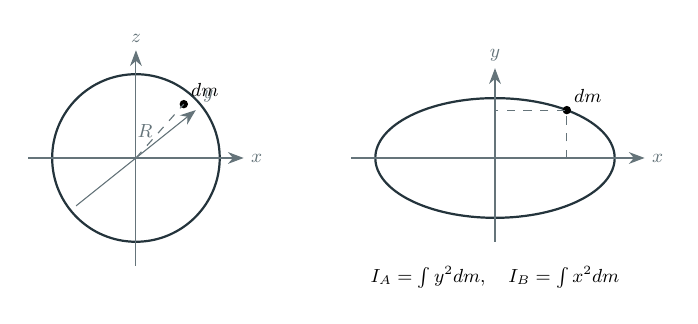
\begin{tikzpicture}[scale=.76,transform shape]

\draw[object] (0,0) circle (1.4);
\draw[axis] (-1.8,0)--(1.8,0) node[right] {$x$};
\draw[axis] (0,-1.8)--(0,1.8) node[above] {$z$};
\draw[axis] (-1,-.8)--(1, .8) node[above right] {$y$};
\fill (.8,.9) circle (2pt) node[above right] {$dm$};
\draw[guide] (0,0)--(.8,.9) node[midway,left] {$R$};
\begin{scope}[xshift=6cm]
\draw[object] (0,0) ellipse (2 and 1);
\draw[axis] (-2.4,0)--(2.5,0) node[right] {$x$};
\draw[axis] (0,-1.4)--(0,1.5) node[above] {$y$};
\fill (1.2,.8) circle (2pt) node[above right] {$dm$};
\draw[guide] (1.2,0)--(1.2,.8)--(0,.8);
\node at (0,-2) {$I_A=\int y^2dm,\quad I_B=\int x^2dm$};
\end{scope}

\end{tikzpicture}
\figcaption{解图综四.1B\quad 球壳三径求和与椭圆上的逐质元几何恒等式。}
\end{minipage}\end{center}
第（2）问，解图综四.1B以球心为原点作三条正交直径。任一质元$dm$的坐标满足$x^2+y^2+z^2=R^2$，所以
\[
I_x=\int(y^2+z^2)dm,\quad
I_y=\int(z^2+x^2)dm,\quad
I_z=\int(x^2+y^2)dm.
\]
相加得
\[
I_x+I_y+I_z=2\int R^2dm=2mR^2.
\]
均匀球壳关于任一直径的惯量相同，$I_x=I_y=I_z=I_R$，故
\[
\boxed{I_R=\frac23mR^2}.
\]
求和时每个坐标平方恰出现两次，所以几何恒等式适用于壳上的每一个质元。其后使用均匀分布的旋转对称性，将三条直径的惯量置为相同，再由总和除以3。这里先作逐质元求和、后使用质量对称性，这两步分别给出$2mR^2$和三径相等。

对解图综四.1B右侧的椭圆细环，取长轴为$x$轴、短轴为$y$轴。每个质元都满足
$x^2/A^2+y^2/B^2=1$，而
\[
I_A=\int y^2dm,\qquad I_B=\int x^2dm.
\]
将几何恒等式按质量积分：
\[
\frac{I_A}{B^2}+\frac{I_B}{A^2}
=\int\left(\frac{y^2}{B^2}+\frac{x^2}{A^2}\right)dm=m.
\]
因此即使质量不均匀，仍有
\[
\boxed{I_B=mA^2-\frac{A^2}{B^2}I_A}.
\]
若弧长线密度为$\lambda(s)$，两项相加后被积函数为$\lambda(s)[x^2/A^2+y^2/B^2]=\lambda(s)$，因此右端恰是总质量。质量偏向长轴端点会增加$I_B$、减小$I_A$，二者始终满足这一线性关系；它保留了题设未指定密度时可确定的全部组合信息。
\begin{center}\begin{minipage}{.98\linewidth}\centering
\begin{tikzpicture}[scale=.85,transform shape]

\begin{scope}[x={(2.2cm,0cm)},y={(1cm,.8cm)},z={(0cm,2.2cm)}]
\draw[object] (0,0,0)--(1,0,0)--(1,0,1)--(0,0,1)--cycle;
\draw[object] (0,0,1)--(0,1,1)--(1,1,1)--(1,0,1);
\draw[object] (1,0,0)--(1,1,0)--(1,1,1);
\draw[guide] (0,0,0)--(0,1,0)--(0,1,1) (0,1,0)--(1,1,0);
\draw[motion] (0,0,0)--(1,1,1);
\node[below left] at (0,0,0) {$P$};\node[above right] at (1,1,1) {$Q$};

\draw[guide] (.5,0,0)--(.5,0,1)--(.5,1,1)--(.5,1,0)--cycle;
\draw[guide] (0,.5,0)--(1,.5,0)--(1,.5,1)--(0,.5,1)--cycle;
\draw[guide] (0,0,.5)--(1,0,.5)--(1,1,.5)--(0,1,.5)--cycle;
\fill[accent] (.25,.25,.25) circle (1.5pt) (.75,.75,.75) circle (1.5pt);
\end{scope}
\node[align=left] at (6,1.7) {两块中心在PQ上\\六块中心偏离PQ\\$I'=\alpha ma^2/32$\\$d=a/\sqrt6$};
\node at (3,-1) {$I=8I'+6(m/8)d^2$};

\end{tikzpicture}
\figcaption{解图综四.1C\quad 八个小立方体共享同一个无量纲惯量系数，偏轴六块再加平移项。}
\end{minipage}\end{center}
第（3）问，立方体只有质量尺度$m$与长度尺度$a$，故绕给定体对角线的惯量应写为
$I=\alpha ma^2$。量纲给不出无量纲常数$\alpha$，还要使用自相似分割。

解图综四.1C将立方体沿三方向各平分成八块。每块质量$m/8$、边长$a/2$，绕自身、平行于$PQ$的体对角线有
\[
I'=\alpha\frac m8\left(\frac a2\right)^2=\frac{\alpha ma^2}{32}.
\]
八个小立方体中两块的中心落在$PQ$上；另外六块中心到$PQ$的垂距相同；每块自己的体对角线方向与大轴平行，正好满足平行轴定理的轴向条件。以大立方体中心为原点，后六个中心坐标是$(\pm a/4,\pm a/4,\pm a/4)$中符号不全相同者。沿$PQ$的单位向量为$(1,1,1)/\sqrt3$，所以
\[
d^2=\frac{3a^2}{16}
-\frac{(a/4)^2}{3}=\frac{a^2}{6}.
\]
解图综四.1D把偏轴小块中心$G$到大轴的垂足$H$标出，$GH$才是平移项所用的距离。由直角分解$GH^2=OG^2-OH^2$得到上式，也可写成$d=(a/2)\sqrt{2/3}=a/\sqrt6$。
\begin{center}\begin{minipage}{.98\linewidth}\centering
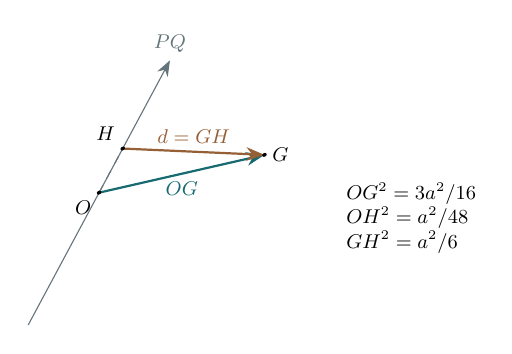
\begin{tikzpicture}[scale=0.8,transform shape]
\begin{scope}[x={(1cm,0cm)},y={(.25cm,.9cm)},z={(-.5cm,.5cm)}]
\coordinate (O) at (0,0,0);\coordinate (G) at (1.5,1.5,-1.5);\coordinate (H) at (.5,.5,.5);
\draw[axis] (-1.5,-1.5,-1.5)--(1.5,1.5,1.5) node[above] {$PQ$};
\draw[motion] (O)--(G) node[midway,below] {$OG$};\draw[guide] (O)--(H);
\draw[force] (H)--(G) node[midway,above] {$d=GH$};
\fill (O) circle(.035) node[below left] {$O$};\fill (G) circle(.035) node[right] {$G$};\fill (H) circle(.035) node[above left] {$H$};\end{scope}
\node[right,align=left] at (3.8,-.4) {$OG^2=3a^2/16$\\$OH^2=a^2/48$\\$GH^2=a^2/6$};\end{tikzpicture}
\figcaption{解图综四.1D\quad 偏轴小块中心向大体对角线投影，平移项取垂距GH的平方}
\end{minipage}\end{center}
每个偏轴小块由平行轴定理增加$(m/8)d^2=ma^2/48$，相加得
\[
I=2I'+6\left(I'+\frac{ma^2}{48}\right)
=8I'+\frac{ma^2}{8}.
\]
代入$I=\alpha ma^2$和$I'=\alpha ma^2/32$，
\[
\alpha=\frac{\alpha}{4}+\frac18,\qquad
\boxed{\alpha=\frac16,\quad I=\frac16ma^2}.
\]
均匀立方体的中心惯量还可由其对称性解释：三坐标方向的二次矩各为$\int x^2\,\mathrm dm=ma^2/12$，故$I_x=I_y=I_z=ma^2/6$。关于中心平面的反射使$\int xy\,\mathrm dm$等混合二次矩为零。对于任意单位轴向$\boldsymbol n$，$I_{\boldsymbol n}=n_x^2I_x+n_y^2I_y+n_z^2I_z=ma^2/6$；因此体对角线与其他中心轴具有相同的惯量。


\Needspace{13\baselineskip}

\pdfbookmark[2]{第 2 题 方截面浮木的平衡与临界稳定性}{q2}

\section*{第 2 题\quad 方截面浮木的平衡与临界稳定性}\label{q:2}


一根均匀长方体木料，其正截面为边长$2a$的正方形，长边始终与水面平行。木料密度为$\rho$，水的密度为$\rho_0$，忽略毛细作用。

（1）给出木料部分露出水面时的平衡条件，说明浮心与重心的几何关系。

（2）木料对称地浮在水面上，正截面的一条对角线竖直，且只有一条长棱没入水中，浸截面是下角的等腰直角三角形。讨论这种姿态对微小转动的稳定性，尤其说明临界密度比时是否随遇平衡。必要的参数可自行定义。


\begin{center}\begin{minipage}{.98\linewidth}\centering
\begin{tikzpicture}[scale=.85,transform shape]

\fill[accent!12] (-1.05,-.364)--(0,-1.414)--(1.05,-.364)--cycle;

\draw[object] (0,-1.414)--(1.414,0)--(0,1.414)--(-1.414,0)--cycle;
\fill (0,0) circle (2pt) node[above right] {$O$};

\draw[axis] (-2,-.364)--(2,-.364) node[right] {水面};
\fill (0,-.714) circle (2pt) node[right] {$C$};
\draw[force] (0,-.714)--(0,.6) node[left] {浮力};
\draw[force,color=warm] (0,0)--(0,-1.3) node[right] {重力};
\node at (0,-2.2) {长边垂直纸面，正截面边长$2a$};

\end{tikzpicture}
\figcaption{图综四.2\quad 对称尖角向下的浮木，浮力作用线通过浸三角形重心。}
\end{minipage}\end{center}

\Needspace{6\baselineskip}\subsection*{解答}


图综四.2取垂直木料长边的截面。整体重心$O$在正方形中心，浸入水中的截面面积为$S$，其几何重心$C$是浮心在本截面的位置。水中静压随深度增加，木料各处压力的合力竖直向上；其大小等于排开水的重力。对于沿长边均匀的柱体，排水体积为$Sb$，浮心的截面坐标由面积一阶矩给出$S\boldsymbol r_C=\int_S\boldsymbol r\,\mathrm dA$。这将水压作用转成通过浸区几何重心的一个竖直力。若木料长为$b$，重力与浮力分别为$4a^2b\rho g$、$Sb\rho_0g$。

第（1）问，部分浸入要求$0<\rho<\rho_0$，平动平衡给
\[
\boxed{S=4a^2\frac{\rho}{\rho_0}}.
\]
重力过$O$、浮力过$C$，二者都竖直。绕$O$无力矩还要求
\[
\boxed{O,C\text{位于同一竖直线上}}.
\]
面积条件保证力的大小，竖直共线条件保证力矩；两项条件须同时满足。对于给定密度，木料的升沉先选出排水面积，随后对不同倾角比较浮心位置，才确定哪些姿态能静止。这个顺序也用于微倾后的稳定性分析：各比较状态先保持同一排水量，再看力矩如何改变倾角。均匀木料水上部分的截面积为$S'=4a^2-S$、重心为$C'$。以$O$作原点，质量加权关系为$S\boldsymbol r_C+S'\boldsymbol r_{C'}=0$，所以$C,O,C'$共线，且$S|OC|=S'|OC'|$。若这条线与实际竖直方向有夹角，两部分重力的合力仍过$O$，浮力则过$C$，留下一项浮力矩$M_B=F_Bx_C$，其中$x_C$是浮心相对于$O$的水平位移。令其为零便得到上面的竖直共线条件。力平衡单独决定排水量，力矩平衡再选择木料姿态；密度条件、排水面积条件和共线条件共同构成第（1）问的平衡要求。
\begin{center}\begin{minipage}{.98\linewidth}\centering
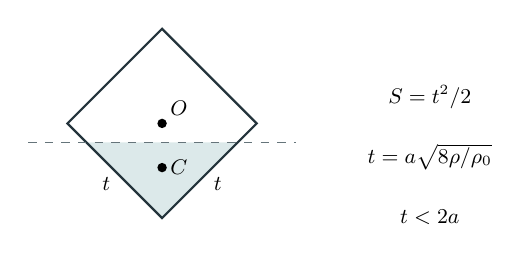
\begin{tikzpicture}[scale=.85,transform shape]

\fill[accent!15] (-1.131,-.283)--(0,-1.414)--(1.131,-.283)--cycle;

\draw[object] (0,-1.414)--(1.414,0)--(0,1.414)--(-1.414,0)--cycle;
\fill (0,0) circle (2pt) node[above right] {$O$};

\draw[guide] (-2,-.283)--(2,-.283);
\node[left] at (-.65,-.9) {$t$};\node[right] at (.65,-.9) {$t$};
\fill (0,-.66) circle (2pt) node[right] {$C$};
\node at (4, .4) {$S=t^2/2$};
\node at (4,-.5) {$t=a\sqrt{8\rho/\rho_0}$};
\node at (4,-1.4) {$t<2a$};

\end{tikzpicture}
\figcaption{解图综四.2A\quad 对称浸区是等腰直角三角形；面积比确定两边浸长。}
\end{minipage}\end{center}
第（2）问，解图综四.2A在对称姿态中令下角沿两边的浸长均为$t$，则
\[
S=\frac{t^2}{2},\qquad t=a\sqrt{\frac{8\rho}{\rho_0}},
\qquad 0<t<2a.
\]
最后一个条件等价于$0<\rho/\rho_0<1/2$，保证只有下方一条长棱浸水。现使木料微倾，并允许它少量升沉以维持浮力等于重力。两侧浸长改为$p,q$，且
\[
\boxed{pq=t^2}.
\]
微倾时木料可在竖直方向稍作平移，水线位置随姿态调节，使所排水的面积保持原值。两边仍相互垂直；在下角建立分别沿两木料侧边的正交坐标$x,y$，三角形顶点为$(0,0),(p,0),(0,q)$，水线为$x/p+y/q=1$。对该区域作面积积分，$\int_Sx\,\mathrm dA=Sp/3$、$\int_Sy\,\mathrm dA=Sq/3$，故浮心为$(p/3,q/3)$。正方形中心$O$在同一坐标中为$(a,a)$。
\begin{center}\begin{minipage}{.98\linewidth}\centering
\begin{tikzpicture}[scale=.85,transform shape]

\coordinate (V) at (0,0);\coordinate (U) at (1.2,0);\coordinate (W) at (0,1.875);
\fill[accent!15] (V)--(U)--(W)--cycle;
\draw[object] (0,0) rectangle (2,2);
\draw[traj] (U)--(W);
\fill (1,1) circle (2pt) node[below right] {$O$};
\fill (.4,.625) circle (2pt) node[left] {$C$};
\draw[guide] (1,1)--(.4,.625);
\draw[force] (.4,.625)--(1.411,1.272);
\draw[guide] (1.411,1.272)--(2.8,2.16096);
\node[above] at (2.8,2.16096) {浮力竖线};
\draw[guide] (1,1)--(1.9,1.576);
\node[below] at (.6,0) {$p$};\node[left] at (0,.94) {$q$};
\node[anchor=west,align=left] at (3.4,1.2) {$O=(a,a),\ C=(p/3,q/3)$\\$pq=t^2$\\$\tan\phi=p/q$\\$\tan\phi'=(a-q/3)/(a-p/3)$};
\node at (2.5,-1) {侧边坐标中水线斜置，竖直方向与水线垂直};

\end{tikzpicture}
\figcaption{解图综四.2B\quad 微倾后三角形浮心及实际竖直方向；本图用木料侧边作坐标。}
\end{minipage}\end{center}
解图综四.2B以一条侧边的法线为参照方向。设过$O$竖直线与该方向夹角为$\phi$，$OC$与同方向夹角为$\phi'$，按图的$p<q$一侧取正，几何关系给
\[
\tan\phi=\frac pq,\qquad
\tan\phi'=\frac{a-q/3}{a-p/3}.
\]
在未倾斜时$p=q=t$，两角相等。倾斜后若$\phi'<\phi$，浮心移到能提供恢复力矩的一侧，为稳定；若$\phi'>\phi$，力矩使扰动继续扩大，为不稳定。

由于$p,q<2a$，分母均为正。比较正切等价于比较
\[
\phi'<\phi
\ \Longleftrightarrow\
p\left(a-\frac p3\right)>
q\left(a-\frac q3\right).
\]
定义$G(z)=az-z^2/3$，它在$z=3a/2$处取最大值。更直接地，
\[
G(p)-G(q)=(p-q)\left(a-\frac{p+q}{3}\right).
\]
这个因式分解也给出浮力矩的具体表达。水线的向上单位法向量在木料坐标中为$\boldsymbol n=(q,p)/\sqrt{p^2+q^2}$，因此浮力为$F_B\boldsymbol n$。以逆时针转动为力矩正向，关于$O$的力矩为
\[
\begin{aligned}
\tau_O&=\frac{F_B}{\sqrt{p^2+q^2}}\left[
p\left(\frac p3-a\right)-q\left(\frac q3-a\right)\right]\\
&=\frac{F_B(p-q)(p+q-3a)}{3\sqrt{p^2+q^2}}
=-\frac{F_B[G(p)-G(q)]}{\sqrt{p^2+q^2}}.
\end{aligned}
\]
选倾转角$\delta$使$p<q$时$\delta>0$，恢复力矩为负。因$p-q<0$，恢复力矩的条件正是$p+q>3a$。解图综四.2D画出三种密度下力矩随倾角的变化，正倾角处的负力矩指向对称姿态，使浮心的角度比较与实际恢复方向对应。
\begin{center}\begin{minipage}{.98\linewidth}\centering
\begin{tikzpicture}[scale=0.72,transform shape]
\draw[axis] (0,0)--(6.2,0);\draw[axis] (0,0)--(0,3.4000000000000004);
\draw[thin,color=muted] (0.0000000,0)--(0.0000000,-.07);\node[below] at (0.0000000,-.09) {$-.15$};
\draw[thin,color=muted] (3.0000000,0)--(3.0000000,-.07);\node[below] at (3.0000000,-.09) {$0$};
\draw[thin,color=muted] (6.0000000,0)--(6.0000000,-.07);\node[below] at (6.0000000,-.09) {$.15$};
\draw[thin,color=muted] (0,0.5333333)--(-.07,0.5333333);\node[left] at (-.09,0.5333333) {$-.02$};
\draw[thin,color=muted] (0,1.6000000)--(-.07,1.6000000);\node[left] at (-.09,1.6000000) {$0$};
\draw[thin,color=muted] (0,2.6666667)--(-.07,2.6666667);\node[left] at (-.09,2.6666667) {$.02$};
\node[below] at (3.0,-.64) {实际倾转角$\delta$（弧度）};\node[above right] at (0,3.45) {$\tau/(F_Ba)$};
\draw[traj] plot coordinates {(0.0000000,1.0788683) (0.0200000,1.0806336) (0.0400000,1.0824345) (0.0600000,1.0842707) (0.0800000,1.0861418) (0.1000000,1.0880477) (0.1200000,1.0899881) (0.1400000,1.0919626) (0.1600000,1.0939710) (0.1800000,1.0960130) (0.2000000,1.0980884) (0.2200000,1.1001968) (0.2400000,1.1023380) (0.2600000,1.1045116) (0.2800000,1.1067176) (0.3000000,1.1089555) (0.3200000,1.1112251) (0.3400000,1.1135261) (0.3600000,1.1158582) (0.3800000,1.1182213) (0.4000000,1.1206149) (0.4200000,1.1230389) (0.4400000,1.1254930) (0.4600000,1.1279769) (0.4800000,1.1304904) (0.5000000,1.1330331) (0.5200000,1.1356049) (0.5400000,1.1382054) (0.5600000,1.1408345) (0.5800000,1.1434917) (0.6000000,1.1461770) (0.6200000,1.1488899) (0.6400000,1.1516304) (0.6600000,1.1543980) (0.6800000,1.1571926) (0.7000000,1.1600139) (0.7200000,1.1628616) (0.7400000,1.1657355) (0.7600000,1.1686353) (0.7800000,1.1715608) (0.8000000,1.1745117) (0.8200000,1.1774878) (0.8400000,1.1804888) (0.8600000,1.1835145) (0.8800000,1.1865645) (0.9000000,1.1896388) (0.9200000,1.1927369) (0.9400000,1.1958588) (0.9600000,1.1990040) (0.9800000,1.2021724) (1.0000000,1.2053638) (1.0200000,1.2085778) (1.0400000,1.2118142) (1.0600000,1.2150729) (1.0800000,1.2183535) (1.1000000,1.2216558) (1.1200000,1.2249795) (1.1400000,1.2283245) (1.1600000,1.2316904) (1.1800000,1.2350771) (1.2000000,1.2384843) (1.2200000,1.2419117) (1.2400000,1.2453591) (1.2600000,1.2488263) (1.2800000,1.2523131) (1.3000000,1.2558191) (1.3200000,1.2593442) (1.3400000,1.2628881) (1.3600000,1.2664506) (1.3800000,1.2700315) (1.4000000,1.2736304) (1.4200000,1.2772472) (1.4400000,1.2808817) (1.4600000,1.2845336) (1.4800000,1.2882026) (1.5000000,1.2918886) (1.5200000,1.2955913) (1.5400000,1.2993105) (1.5600000,1.3030459) (1.5800000,1.3067973) (1.6000000,1.3105645) (1.6200000,1.3143472) (1.6400000,1.3181452) (1.6600000,1.3219583) (1.6800000,1.3257863) (1.7000000,1.3296289) (1.7200000,1.3334859) (1.7400000,1.3373571) (1.7600000,1.3412422) (1.7800000,1.3451410) (1.8000000,1.3490533) (1.8200000,1.3529788) (1.8400000,1.3569174) (1.8600000,1.3608687) (1.8800000,1.3648327) (1.9000000,1.3688089) (1.9200000,1.3727973) (1.9400000,1.3767976) (1.9600000,1.3808096) (1.9800000,1.3848330) (2.0000000,1.3888676) (2.0200000,1.3929132) (2.0400000,1.3969696) (2.0600000,1.4010366) (2.0800000,1.4051138) (2.1000000,1.4092012) (2.1200000,1.4132984) (2.1400000,1.4174053) (2.1600000,1.4215216) (2.1800000,1.4256471) (2.2000000,1.4297816) (2.2200000,1.4339249) (2.2400000,1.4380767) (2.2600000,1.4422368) (2.2800000,1.4464051) (2.3000000,1.4505812) (2.3200000,1.4547649) (2.3400000,1.4589561) (2.3600000,1.4631545) (2.3800000,1.4673599) (2.4000000,1.4715721) (2.4200000,1.4757909) (2.4400000,1.4800159) (2.4600000,1.4842471) (2.4800000,1.4884842) (2.5000000,1.4927269) (2.5200000,1.4969751) (2.5400000,1.5012286) (2.5600000,1.5054870) (2.5800000,1.5097503) (2.6000000,1.5140181) (2.6200000,1.5182903) (2.6400000,1.5225666) (2.6600000,1.5268469) (2.6800000,1.5311308) (2.7000000,1.5354183) (2.7200000,1.5397090) (2.7400000,1.5440028) (2.7600000,1.5482993) (2.7800000,1.5525986) (2.8000000,1.5569002) (2.8200000,1.5612039) (2.8400000,1.5655097) (2.8600000,1.5698172) (2.8800000,1.5741262) (2.9000000,1.5784365) (2.9200000,1.5827479) (2.9400000,1.5870601) (2.9600000,1.5913731) (2.9800000,1.5956864) (3.0000000,1.6000000) (3.0200000,1.6043136) (3.0400000,1.6086269) (3.0600000,1.6129399) (3.0800000,1.6172521) (3.1000000,1.6215635) (3.1200000,1.6258738) (3.1400000,1.6301828) (3.1600000,1.6344903) (3.1800000,1.6387961) (3.2000000,1.6430998) (3.2200000,1.6474014) (3.2400000,1.6517007) (3.2600000,1.6559972) (3.2800000,1.6602910) (3.3000000,1.6645817) (3.3200000,1.6688692) (3.3400000,1.6731531) (3.3600000,1.6774334) (3.3800000,1.6817097) (3.4000000,1.6859819) (3.4200000,1.6902497) (3.4400000,1.6945130) (3.4600000,1.6987714) (3.4800000,1.7030249) (3.5000000,1.7072731) (3.5200000,1.7115158) (3.5400000,1.7157529) (3.5600000,1.7199841) (3.5800000,1.7242091) (3.6000000,1.7284279) (3.6200000,1.7326401) (3.6400000,1.7368455) (3.6600000,1.7410439) (3.6800000,1.7452351) (3.7000000,1.7494188) (3.7200000,1.7535949) (3.7400000,1.7577632) (3.7600000,1.7619233) (3.7800000,1.7660751) (3.8000000,1.7702184) (3.8200000,1.7743529) (3.8400000,1.7784784) (3.8600000,1.7825947) (3.8800000,1.7867016) (3.9000000,1.7907988) (3.9200000,1.7948862) (3.9400000,1.7989634) (3.9600000,1.8030304) (3.9800000,1.8070868) (4.0000000,1.8111324) (4.0200000,1.8151670) (4.0400000,1.8191904) (4.0600000,1.8232024) (4.0800000,1.8272027) (4.1000000,1.8311911) (4.1200000,1.8351673) (4.1400000,1.8391313) (4.1600000,1.8430826) (4.1800000,1.8470212) (4.2000000,1.8509467) (4.2200000,1.8548590) (4.2400000,1.8587578) (4.2600000,1.8626429) (4.2800000,1.8665141) (4.3000000,1.8703711) (4.3200000,1.8742137) (4.3400000,1.8780417) (4.3600000,1.8818548) (4.3800000,1.8856528) (4.4000000,1.8894355) (4.4200000,1.8932027) (4.4400000,1.8969541) (4.4600000,1.9006895) (4.4800000,1.9044087) (4.5000000,1.9081114) (4.5200000,1.9117974) (4.5400000,1.9154664) (4.5600000,1.9191183) (4.5800000,1.9227528) (4.6000000,1.9263696) (4.6200000,1.9299685) (4.6400000,1.9335494) (4.6600000,1.9371119) (4.6800000,1.9406558) (4.7000000,1.9441809) (4.7200000,1.9476869) (4.7400000,1.9511737) (4.7600000,1.9546409) (4.7800000,1.9580883) (4.8000000,1.9615157) (4.8200000,1.9649229) (4.8400000,1.9683096) (4.8600000,1.9716755) (4.8800000,1.9750205) (4.9000000,1.9783442) (4.9200000,1.9816465) (4.9400000,1.9849271) (4.9600000,1.9881858) (4.9800000,1.9914222) (5.0000000,1.9946362) (5.0200000,1.9978276) (5.0400000,2.0009960) (5.0600000,2.0041412) (5.0800000,2.0072631) (5.1000000,2.0103612) (5.1200000,2.0134355) (5.1400000,2.0164855) (5.1600000,2.0195112) (5.1800000,2.0225122) (5.2000000,2.0254883) (5.2200000,2.0284392) (5.2400000,2.0313647) (5.2600000,2.0342645) (5.2800000,2.0371384) (5.3000000,2.0399861) (5.3200000,2.0428074) (5.3400000,2.0456020) (5.3600000,2.0483696) (5.3800000,2.0511101) (5.4000000,2.0538230) (5.4200000,2.0565083) (5.4400000,2.0591655) (5.4600000,2.0617946) (5.4800000,2.0643951) (5.5000000,2.0669669) (5.5200000,2.0695096) (5.5400000,2.0720231) (5.5600000,2.0745070) (5.5800000,2.0769611) (5.6000000,2.0793851) (5.6200000,2.0817787) (5.6400000,2.0841418) (5.6600000,2.0864739) (5.6800000,2.0887749) (5.7000000,2.0910445) (5.7200000,2.0932824) (5.7400000,2.0954884) (5.7600000,2.0976620) (5.7800000,2.0998032) (5.8000000,2.1019116) (5.8200000,2.1039870) (5.8400000,2.1060290) (5.8600000,2.1080374) (5.8800000,2.1100119) (5.9000000,2.1119523) (5.9200000,2.1138582) (5.9400000,2.1157293) (5.9600000,2.1175655) (5.9800000,2.1193664) (6.0000000,2.1211317)};
\draw[traj] (.1,-1.05)--(.7,-1.05);\node[right] at (.85,-1.05) {密度比$1/4$};\draw[dashed,thick,color=warm] plot coordinates {(0.0000000,1.7309772) (0.0200000,1.7283253) (0.0400000,1.7257105) (0.0600000,1.7231325) (0.0800000,1.7205909) (0.1000000,1.7180855) (0.1200000,1.7156159) (0.1400000,1.7131820) (0.1600000,1.7107833) (0.1800000,1.7084196) (0.2000000,1.7060907) (0.2200000,1.7037961) (0.2400000,1.7015357) (0.2600000,1.6993092) (0.2800000,1.6971162) (0.3000000,1.6949565) (0.3200000,1.6928298) (0.3400000,1.6907359) (0.3600000,1.6886743) (0.3800000,1.6866449) (0.4000000,1.6846474) (0.4200000,1.6826815) (0.4400000,1.6807469) (0.4600000,1.6788433) (0.4800000,1.6769705) (0.5000000,1.6751282) (0.5200000,1.6733161) (0.5400000,1.6715340) (0.5600000,1.6697815) (0.5800000,1.6680584) (0.6000000,1.6663645) (0.6200000,1.6646994) (0.6400000,1.6630628) (0.6600000,1.6614546) (0.6800000,1.6598745) (0.7000000,1.6583221) (0.7200000,1.6567972) (0.7400000,1.6552996) (0.7600000,1.6538290) (0.7800000,1.6523851) (0.8000000,1.6509676) (0.8200000,1.6495764) (0.8400000,1.6482110) (0.8600000,1.6468714) (0.8800000,1.6455571) (0.9000000,1.6442680) (0.9200000,1.6430038) (0.9400000,1.6417642) (0.9600000,1.6405489) (0.9800000,1.6393578) (1.0000000,1.6381906) (1.0200000,1.6370469) (1.0400000,1.6359266) (1.0600000,1.6348293) (1.0800000,1.6337550) (1.1000000,1.6327031) (1.1200000,1.6316736) (1.1400000,1.6306662) (1.1600000,1.6296806) (1.1800000,1.6287166) (1.2000000,1.6277739) (1.2200000,1.6268523) (1.2400000,1.6259515) (1.2600000,1.6250712) (1.2800000,1.6242113) (1.3000000,1.6233714) (1.3200000,1.6225514) (1.3400000,1.6217510) (1.3600000,1.6209698) (1.3800000,1.6202078) (1.4000000,1.6194646) (1.4200000,1.6187400) (1.4400000,1.6180338) (1.4600000,1.6173456) (1.4800000,1.6166753) (1.5000000,1.6160227) (1.5200000,1.6153874) (1.5400000,1.6147692) (1.5600000,1.6141680) (1.5800000,1.6135833) (1.6000000,1.6130151) (1.6200000,1.6124631) (1.6400000,1.6119270) (1.6600000,1.6114065) (1.6800000,1.6109016) (1.7000000,1.6104118) (1.7200000,1.6099370) (1.7400000,1.6094769) (1.7600000,1.6090313) (1.7800000,1.6086000) (1.8000000,1.6081827) (1.8200000,1.6077792) (1.8400000,1.6073892) (1.8600000,1.6070126) (1.8800000,1.6066490) (1.9000000,1.6062982) (1.9200000,1.6059601) (1.9400000,1.6056343) (1.9600000,1.6053207) (1.9800000,1.6050189) (2.0000000,1.6047288) (2.0200000,1.6044502) (2.0400000,1.6041827) (2.0600000,1.6039263) (2.0800000,1.6036805) (2.1000000,1.6034453) (2.1200000,1.6032203) (2.1400000,1.6030053) (2.1600000,1.6028002) (2.1800000,1.6026046) (2.2000000,1.6024184) (2.2200000,1.6022413) (2.2400000,1.6020731) (2.2600000,1.6019135) (2.2800000,1.6017624) (2.3000000,1.6016194) (2.3200000,1.6014844) (2.3400000,1.6013571) (2.3600000,1.6012373) (2.3800000,1.6011248) (2.4000000,1.6010194) (2.4200000,1.6009207) (2.4400000,1.6008287) (2.4600000,1.6007430) (2.4800000,1.6006634) (2.5000000,1.6005897) (2.5200000,1.6005217) (2.5400000,1.6004591) (2.5600000,1.6004018) (2.5800000,1.6003494) (2.6000000,1.6003018) (2.6200000,1.6002588) (2.6400000,1.6002200) (2.6600000,1.6001853) (2.6800000,1.6001545) (2.7000000,1.6001273) (2.7200000,1.6001035) (2.7400000,1.6000829) (2.7600000,1.6000652) (2.7800000,1.6000502) (2.8000000,1.6000377) (2.8200000,1.6000275) (2.8400000,1.6000193) (2.8600000,1.6000129) (2.8800000,1.6000081) (2.9000000,1.6000047) (2.9200000,1.6000024) (2.9400000,1.6000010) (2.9600000,1.6000003) (2.9800000,1.6000000) (3.0000000,1.6000000) (3.0200000,1.6000000) (3.0400000,1.5999997) (3.0600000,1.5999990) (3.0800000,1.5999976) (3.1000000,1.5999953) (3.1200000,1.5999919) (3.1400000,1.5999871) (3.1600000,1.5999807) (3.1800000,1.5999725) (3.2000000,1.5999623) (3.2200000,1.5999498) (3.2400000,1.5999348) (3.2600000,1.5999171) (3.2800000,1.5998965) (3.3000000,1.5998727) (3.3200000,1.5998455) (3.3400000,1.5998147) (3.3600000,1.5997800) (3.3800000,1.5997412) (3.4000000,1.5996982) (3.4200000,1.5996506) (3.4400000,1.5995982) (3.4600000,1.5995409) (3.4800000,1.5994783) (3.5000000,1.5994103) (3.5200000,1.5993366) (3.5400000,1.5992570) (3.5600000,1.5991713) (3.5800000,1.5990793) (3.6000000,1.5989806) (3.6200000,1.5988752) (3.6400000,1.5987627) (3.6600000,1.5986429) (3.6800000,1.5985156) (3.7000000,1.5983806) (3.7200000,1.5982376) (3.7400000,1.5980865) (3.7600000,1.5979269) (3.7800000,1.5977587) (3.8000000,1.5975816) (3.8200000,1.5973954) (3.8400000,1.5971998) (3.8600000,1.5969947) (3.8800000,1.5967797) (3.9000000,1.5965547) (3.9200000,1.5963195) (3.9400000,1.5960737) (3.9600000,1.5958173) (3.9800000,1.5955498) (4.0000000,1.5952712) (4.0200000,1.5949811) (4.0400000,1.5946793) (4.0600000,1.5943657) (4.0800000,1.5940399) (4.1000000,1.5937018) (4.1200000,1.5933510) (4.1400000,1.5929874) (4.1600000,1.5926108) (4.1800000,1.5922208) (4.2000000,1.5918173) (4.2200000,1.5914000) (4.2400000,1.5909687) (4.2600000,1.5905231) (4.2800000,1.5900630) (4.3000000,1.5895882) (4.3200000,1.5890984) (4.3400000,1.5885935) (4.3600000,1.5880730) (4.3800000,1.5875369) (4.4000000,1.5869849) (4.4200000,1.5864167) (4.4400000,1.5858320) (4.4600000,1.5852308) (4.4800000,1.5846126) (4.5000000,1.5839773) (4.5200000,1.5833247) (4.5400000,1.5826544) (4.5600000,1.5819662) (4.5800000,1.5812600) (4.6000000,1.5805354) (4.6200000,1.5797922) (4.6400000,1.5790302) (4.6600000,1.5782490) (4.6800000,1.5774486) (4.7000000,1.5766286) (4.7200000,1.5757887) (4.7400000,1.5749288) (4.7600000,1.5740485) (4.7800000,1.5731477) (4.8000000,1.5722261) (4.8200000,1.5712834) (4.8400000,1.5703194) (4.8600000,1.5693338) (4.8800000,1.5683264) (4.9000000,1.5672969) (4.9200000,1.5662450) (4.9400000,1.5651707) (4.9600000,1.5640734) (4.9800000,1.5629531) (5.0000000,1.5618094) (5.0200000,1.5606422) (5.0400000,1.5594511) (5.0600000,1.5582358) (5.0800000,1.5569962) (5.1000000,1.5557320) (5.1200000,1.5544429) (5.1400000,1.5531286) (5.1600000,1.5517890) (5.1800000,1.5504236) (5.2000000,1.5490324) (5.2200000,1.5476149) (5.2400000,1.5461710) (5.2600000,1.5447004) (5.2800000,1.5432028) (5.3000000,1.5416779) (5.3200000,1.5401255) (5.3400000,1.5385454) (5.3600000,1.5369372) (5.3800000,1.5353006) (5.4000000,1.5336355) (5.4200000,1.5319416) (5.4400000,1.5302185) (5.4600000,1.5284660) (5.4800000,1.5266839) (5.5000000,1.5248718) (5.5200000,1.5230295) (5.5400000,1.5211567) (5.5600000,1.5192531) (5.5800000,1.5173185) (5.6000000,1.5153526) (5.6200000,1.5133551) (5.6400000,1.5113257) (5.6600000,1.5092641) (5.6800000,1.5071702) (5.7000000,1.5050435) (5.7200000,1.5028838) (5.7400000,1.5006908) (5.7600000,1.4984643) (5.7800000,1.4962039) (5.8000000,1.4939093) (5.8200000,1.4915804) (5.8400000,1.4892167) (5.8600000,1.4868180) (5.8800000,1.4843841) (5.9000000,1.4819145) (5.9200000,1.4794091) (5.9400000,1.4768675) (5.9600000,1.4742895) (5.9800000,1.4716747) (6.0000000,1.4690228)};
\draw[dashed,thick,color=warm] (.1,-1.48)--(.7,-1.48);\node[right] at (.85,-1.48) {密度比$9/32$};\draw[dotted,thick,color=muted] plot coordinates {(0.0000000,2.7419297) (0.0200000,2.7324301) (0.0400000,2.7229697) (0.0600000,2.7135484) (0.0800000,2.7041658) (0.1000000,2.6948216) (0.1200000,2.6855154) (0.1400000,2.6762471) (0.1600000,2.6670162) (0.1800000,2.6578225) (0.2000000,2.6486657) (0.2200000,2.6395453) (0.2400000,2.6304612) (0.2600000,2.6214131) (0.2800000,2.6124006) (0.3000000,2.6034234) (0.3200000,2.5944812) (0.3400000,2.5855738) (0.3600000,2.5767007) (0.3800000,2.5678618) (0.4000000,2.5590568) (0.4200000,2.5502852) (0.4400000,2.5415469) (0.4600000,2.5328416) (0.4800000,2.5241688) (0.5000000,2.5155285) (0.5200000,2.5069202) (0.5400000,2.4983436) (0.5600000,2.4897986) (0.5800000,2.4812847) (0.6000000,2.4728017) (0.6200000,2.4643494) (0.6400000,2.4559273) (0.6600000,2.4475353) (0.6800000,2.4391731) (0.7000000,2.4308403) (0.7200000,2.4225367) (0.7400000,2.4142620) (0.7600000,2.4060160) (0.7800000,2.3977983) (0.8000000,2.3896086) (0.8200000,2.3814467) (0.8400000,2.3733123) (0.8600000,2.3652052) (0.8800000,2.3571250) (0.9000000,2.3490714) (0.9200000,2.3410443) (0.9400000,2.3330432) (0.9600000,2.3250681) (0.9800000,2.3171184) (1.0000000,2.3091941) (1.0200000,2.3012948) (1.0400000,2.2934203) (1.0600000,2.2855702) (1.0800000,2.2777443) (1.1000000,2.2699424) (1.1200000,2.2621642) (1.1400000,2.2544093) (1.1600000,2.2466776) (1.1800000,2.2389688) (1.2000000,2.2312826) (1.2200000,2.2236187) (1.2400000,2.2159768) (1.2600000,2.2083568) (1.2800000,2.2007583) (1.3000000,2.1931811) (1.3200000,2.1856250) (1.3400000,2.1780895) (1.3600000,2.1705746) (1.3800000,2.1630799) (1.4000000,2.1556051) (1.4200000,2.1481501) (1.4400000,2.1407145) (1.4600000,2.1332981) (1.4800000,2.1259006) (1.5000000,2.1185218) (1.5200000,2.1111614) (1.5400000,2.1038192) (1.5600000,2.0964949) (1.5800000,2.0891882) (1.6000000,2.0818989) (1.6200000,2.0746268) (1.6400000,2.0673715) (1.6600000,2.0601328) (1.6800000,2.0529105) (1.7000000,2.0457044) (1.7200000,2.0385141) (1.7400000,2.0313394) (1.7600000,2.0241800) (1.7800000,2.0170358) (1.8000000,2.0099064) (1.8200000,2.0027916) (1.8400000,1.9956912) (1.8600000,1.9886049) (1.8800000,1.9815324) (1.9000000,1.9744736) (1.9200000,1.9674280) (1.9400000,1.9603956) (1.9600000,1.9533761) (1.9800000,1.9463691) (2.0000000,1.9393745) (2.0200000,1.9323921) (2.0400000,1.9254215) (2.0600000,1.9184625) (2.0800000,1.9115148) (2.1000000,1.9045783) (2.1200000,1.8976527) (2.1400000,1.8907377) (2.1600000,1.8838331) (2.1800000,1.8769387) (2.2000000,1.8700541) (2.2200000,1.8631792) (2.2400000,1.8563137) (2.2600000,1.8494574) (2.2800000,1.8426100) (2.3000000,1.8357712) (2.3200000,1.8289409) (2.3400000,1.8221188) (2.3600000,1.8153046) (2.3800000,1.8084981) (2.4000000,1.8016991) (2.4200000,1.7949073) (2.4400000,1.7881225) (2.4600000,1.7813444) (2.4800000,1.7745728) (2.5000000,1.7678075) (2.5200000,1.7610481) (2.5400000,1.7542945) (2.5600000,1.7475465) (2.5800000,1.7408037) (2.6000000,1.7340660) (2.6200000,1.7273331) (2.6400000,1.7206047) (2.6600000,1.7138807) (2.6800000,1.7071607) (2.7000000,1.7004446) (2.7200000,1.6937320) (2.7400000,1.6870229) (2.7600000,1.6803168) (2.7800000,1.6736136) (2.8000000,1.6669131) (2.8200000,1.6602150) (2.8400000,1.6535190) (2.8600000,1.6468249) (2.8800000,1.6401325) (2.9000000,1.6334416) (2.9200000,1.6267518) (2.9400000,1.6200630) (2.9600000,1.6133749) (2.9800000,1.6066874) (3.0000000,1.6000000) (3.0200000,1.5933126) (3.0400000,1.5866251) (3.0600000,1.5799370) (3.0800000,1.5732482) (3.1000000,1.5665584) (3.1200000,1.5598675) (3.1400000,1.5531751) (3.1600000,1.5464810) (3.1800000,1.5397850) (3.2000000,1.5330869) (3.2200000,1.5263864) (3.2400000,1.5196832) (3.2600000,1.5129771) (3.2800000,1.5062680) (3.3000000,1.4995554) (3.3200000,1.4928393) (3.3400000,1.4861193) (3.3600000,1.4793953) (3.3800000,1.4726669) (3.4000000,1.4659340) (3.4200000,1.4591963) (3.4400000,1.4524535) (3.4600000,1.4457055) (3.4800000,1.4389519) (3.5000000,1.4321925) (3.5200000,1.4254272) (3.5400000,1.4186556) (3.5600000,1.4118775) (3.5800000,1.4050927) (3.6000000,1.3983009) (3.6200000,1.3915019) (3.6400000,1.3846954) (3.6600000,1.3778812) (3.6800000,1.3710591) (3.7000000,1.3642288) (3.7200000,1.3573900) (3.7400000,1.3505426) (3.7600000,1.3436863) (3.7800000,1.3368208) (3.8000000,1.3299459) (3.8200000,1.3230613) (3.8400000,1.3161669) (3.8600000,1.3092623) (3.8800000,1.3023473) (3.9000000,1.2954217) (3.9200000,1.2884852) (3.9400000,1.2815375) (3.9600000,1.2745785) (3.9800000,1.2676079) (4.0000000,1.2606255) (4.0200000,1.2536309) (4.0400000,1.2466239) (4.0600000,1.2396044) (4.0800000,1.2325720) (4.1000000,1.2255264) (4.1200000,1.2184676) (4.1400000,1.2113951) (4.1600000,1.2043088) (4.1800000,1.1972084) (4.2000000,1.1900936) (4.2200000,1.1829642) (4.2400000,1.1758200) (4.2600000,1.1686606) (4.2800000,1.1614859) (4.3000000,1.1542956) (4.3200000,1.1470895) (4.3400000,1.1398672) (4.3600000,1.1326285) (4.3800000,1.1253732) (4.4000000,1.1181011) (4.4200000,1.1108118) (4.4400000,1.1035051) (4.4600000,1.0961808) (4.4800000,1.0888386) (4.5000000,1.0814782) (4.5200000,1.0740994) (4.5400000,1.0667019) (4.5600000,1.0592855) (4.5800000,1.0518499) (4.6000000,1.0443949) (4.6200000,1.0369201) (4.6400000,1.0294254) (4.6600000,1.0219105) (4.6800000,1.0143750) (4.7000000,1.0068189) (4.7200000,0.9992417) (4.7400000,0.9916432) (4.7600000,0.9840232) (4.7800000,0.9763813) (4.8000000,0.9687174) (4.8200000,0.9610312) (4.8400000,0.9533224) (4.8600000,0.9455907) (4.8800000,0.9378358) (4.9000000,0.9300576) (4.9200000,0.9222557) (4.9400000,0.9144298) (4.9600000,0.9065797) (4.9800000,0.8987052) (5.0000000,0.8908059) (5.0200000,0.8828816) (5.0400000,0.8749319) (5.0600000,0.8669568) (5.0800000,0.8589557) (5.1000000,0.8509286) (5.1200000,0.8428750) (5.1400000,0.8347948) (5.1600000,0.8266877) (5.1800000,0.8185533) (5.2000000,0.8103914) (5.2200000,0.8022017) (5.2400000,0.7939840) (5.2600000,0.7857380) (5.2800000,0.7774633) (5.3000000,0.7691597) (5.3200000,0.7608269) (5.3400000,0.7524647) (5.3600000,0.7440727) (5.3800000,0.7356506) (5.4000000,0.7271983) (5.4200000,0.7187153) (5.4400000,0.7102014) (5.4600000,0.7016564) (5.4800000,0.6930798) (5.5000000,0.6844715) (5.5200000,0.6758312) (5.5400000,0.6671584) (5.5600000,0.6584531) (5.5800000,0.6497148) (5.6000000,0.6409432) (5.6200000,0.6321382) (5.6400000,0.6232993) (5.6600000,0.6144262) (5.6800000,0.6055188) (5.7000000,0.5965766) (5.7200000,0.5875994) (5.7400000,0.5785869) (5.7600000,0.5695388) (5.7800000,0.5604547) (5.8000000,0.5513343) (5.8200000,0.5421775) (5.8400000,0.5329838) (5.8600000,0.5237529) (5.8800000,0.5144846) (5.9000000,0.5051784) (5.9200000,0.4958342) (5.9400000,0.4864516) (5.9600000,0.4770303) (5.9800000,0.4675699) (6.0000000,0.4580703)};
\draw[dotted,thick,color=muted] (.1,-1.9100000000000001)--(.7,-1.9100000000000001);\node[right] at (.85,-1.9100000000000001) {密度比$1/3$};\end{tikzpicture}
\figcaption{解图综四.2D\quad 正角处负力矩恢复到对称姿态，临界曲线的领先项为三次}
\end{minipage}\end{center}
\begin{center}\begin{minipage}{.98\linewidth}\centering
\begin{tikzpicture}[scale=.85,transform shape]

\draw[axis] (0,0)--(6.5,0) node[right] {$z/a$};
\draw[axis] (0,0)--(0,3.2) node[above] {$G(z)/a^2$};
\draw[traj,domain=0:2.8,samples=100] plot ({2*\x},{3*(\x-\x*\x/3)});
\draw[guide] (3,0)--(3,2.25);
\node[below] at (3,0) {$3/2$};
\node at (4.8,3) {$G(z)=az-z^2/3$};
\node at (3,-1) {$G(p)-G(q)=(p-q)[a-(p+q)/3]$};
\node at (3,-2) {临界时$pq=(3a/2)^2$且$p+q>3a$，仍有恢复力};

\end{tikzpicture}
\figcaption{解图综四.2C\quad 抛物线判据与临界的固定面积约束，三阶项决定临界处的恢复力矩。}
\end{minipage}\end{center}
解图综四.2C比较抛物线上两点。若$t>3a/2$，任意足够小倾斜仍有$p+q>3a$，稳定；若$t<3a/2$，小倾斜后仍有$p+q<3a$，不稳定。临界$t=3a/2$时，一阶恢复系数为零，固定面积约束下的高阶浮心移动决定恢复方向。因为$pq=t^2$固定且$p\ne q$，算术几何平均不等式给
\[
p+q>2\sqrt{pq}=3a,
\]
也可按抛物线的左右位移理解这一结论。设$p=t-\Delta p$，由面积保持得$q=t^2/(t-\Delta p)=t+\Delta q$，其中$\Delta q=t\Delta p/(t-\Delta p)>\Delta p$。在临界$t=3a/2$处，抛物线关于顶点对称，右侧较大的位移使$G(q)$更低，于是$G(p)>G(q)$。所以临界处仍有恢复力矩，只是领先阶较高，它也是稳定平衡。

将$t=a\sqrt{8\rho/\rho_0}$代入，结论为
\[
\boxed{\begin{array}{ll}
0<\rho/\rho_0<9/32:&\text{不稳定},\\
9/32\le\rho/\rho_0<1/2:&\text{稳定}.
\end{array}}
\]
还可令$p=t e^{-\varepsilon},q=t e^\varepsilon$，把面积约束精确保留。在临界$t=3a/2$处，
\[
G(p)-G(q)
=(-2t\sinh\varepsilon)
\left[a-\frac{2t\cosh\varepsilon}{3}\right]
=2at\sinh\varepsilon(\cosh\varepsilon-1)
\sim at\,\varepsilon^3>0.
\]
由力矩式还可定出这一高阶量的物理系数。此时$\sqrt{p^2+q^2}\simeq\sqrt2t$，因此$\tau_O\simeq-F_Ba\varepsilon^3/\sqrt2$。实际倾转角满足$\delta=\arctan(q/p)-\pi/4=\arctan(e^{2\varepsilon})-\pi/4=\varepsilon+O(\varepsilon^3)$，故领先恢复力矩也写成$-F_Ba\delta^3/\sqrt2$。由解图综四.2C 的对称点出发，沿保持浸面积不变的路径积分 $\mathrm dU=-\tau_O\,\mathrm d\delta$，得到
\[
U(\delta)-U(0)=\frac{F_Ba}{4\sqrt2}\,\delta^4+o(\delta^4).
\]
临界时，一阶刚度为零；向左右任一侧微倾，四阶项都使势能增大，因此对称姿态仍是局部极小。上面取的是$p<q$的一侧；关于竖直对角线作镜像时，$p,q$互换，力矩随之反号，倾转角也反号，所以两侧扰动都受到指向对称姿态的恢复作用。

例如密度比为$1/4$时$t=\sqrt2a$，位于临界浸长以下，对称尖角姿态受扰后继续偏转；密度比为$1/3$时$t=\sqrt{8/3}a$，已经超过$3a/2$而仍小于$2a$，恢复力矩使木料回向对称姿态。

线性项也能用稳心高度解释。对称水线宽$w=\sqrt2t$，单位木料长度的水线二次矩为$w^3/12$，除以浸面积$S=t^2/2$得$BM=\sqrt2t/3$。浮心到重心的竖直距离为$BG=\sqrt2(a-t/3)$，因而$GM=BM-BG=\sqrt2(2t/3-a)$。小角浮力矩的一阶项为$-F_BGM\,\delta$，在$t>3a/2$时为恢复项，在$t<3a/2$时使扰动增大；临界点按上面的三阶项判定。以上局部扰动始终保持$p,q<2a$和三角形浸区。水线继续移动而碰到其他棱时，排水截面变为另一多边形，其浮心再按对应几何求取。


\Needspace{13\baselineskip}

\pdfbookmark[2]{第 3 题 滑动悬点细杆的周期与整体落地}{q3}

\section*{第 3 题\quad 滑动悬点细杆的周期与整体落地}\label{q:3}


质量$m$、长$2l$的均匀细杆，其上端$A$套在水平光滑横梁上，可无摩擦滑动。开始时细杆静止，与竖直方向夹$60^\circ$，杆的下端在$A$左下方；$A$距横梁左端为$S$。横梁距水平地面高度为$h$。

（1）若$S$足够大，细杆可完整往复摆动。比较其周期与长$1.1l$、上端固定、振幅也为$60^\circ$的单摆周期，不作小角度近似。

（2）若细杆恰在竖直最低位置时，上端$A$从横梁左端脱出，求相应的$S$。要使杆上各部分同时向下落到地面，$h$应取哪些值？同时说明各候选高度下杆端在此前是否触地。


\begin{center}\begin{minipage}{.98\linewidth}\centering
\begin{tikzpicture}[scale=.85,transform shape]

\draw[object] (-2,0)--(3.5,0);
\fill (1.2,0) circle (3pt) node[above] {$A$};
\draw[object,line width=1.5pt] (1.2,0)--(-1.8,-1.732);
\fill (-.3,-.866) circle (2pt) node[below] {$C$};
\draw[guide] (1.2,0)--(1.2,-2.5);
\draw[guide] (1.2,-.8) arc[start angle=-90,end angle=-150,radius=.8];
\node at (.6,-1) {$60^\circ$};
\draw[axis,<->] (-2,.6)--(1.2,.6) node[midway,above] {$S$};

\draw[object] (-2.5,-4)--(3.6,-4);
\draw[axis,<->] (3.2,0)--(3.2,-4) node[midway,right] {$h$};
\node at (-.6,-2.6) {均匀杆长$2l$};

\end{tikzpicture}
\figcaption{图综四.3\quad 上端可沿梁滑动；杆到竖直最低位置时可从左端脱出。}
\end{minipage}\end{center}

\Needspace{6\baselineskip}\subsection*{解答}


图综四.3以杆中点$C$为质心，取$\phi$为从竖直向下方向量起的杆偏角，初始$\phi=-\pi/3$。横梁无摩擦，其对杆的力竖直，所以系统水平动量始终为零，$C$没有水平位移。
\begin{center}\begin{minipage}{.98\linewidth}\centering
\begin{tikzpicture}[scale=.85,transform shape]

\draw[object] (-2.5,0)--(2.5,0);
\draw[guide] (0,.5)--(0,-3);
\draw[object,line width=1.5pt] (1.2,0)--(-1.2,-2);
\fill (1.2,0) circle (2pt) node[above] {$A$};
\fill (0,-1) circle (2pt) node[left] {$C$};
\draw[guide] (1.2,0)--(1.2,-2.7);
\node at (.6,-.75) {$\phi$};
\draw[motion] (1.2,.3)--(.2,.3);
\draw[motion] (.3,-1)--(.3,-2) node[right] {$v_C$};
\node[align=left] at (5,-1) {$x_C=\text{常量}$\\$y_C=l\cos\phi$\\$v_C=-l\omega\sin\phi$};

\end{tikzpicture}
\figcaption{解图综四.3A\quad 质心沿固定竖线运动，动能中须保留质心平动和绕质心转动。}
\end{minipage}\end{center}
均匀细杆的重力作用在中点，横梁通过套环给竖直约束力，二者在水平方向的分量都为零。杆初始静止，故质心的水平速度从零开始保持为零。取$y$向下为正，杆的几何关系为$x_C=x_A+l\sin\phi$；因此$x_A=x_C-l\sin\phi$，滑动端的移动恰与杆倾斜造成的中点相对位移相反。第（1）问，解图综四.3A中$C$到梁的竖直距离为$y_C=l\cos\phi$，于是
\[
v_C=\dot y_C=-l\dot\phi\sin\phi,\qquad
I_C=\frac1{12}m(2l)^2=\frac13ml^2.
\]
把任一质元的速度分成质心速度与相对转动速度，交叉项的质量积分因$\int\boldsymbol r'\,\mathrm dm=0$而消去，所以总动能为$mv_C^2/2+I_C\dot\phi^2/2$。这里的滑动端并非固定转轴，质心速度由上述约束单独计算。横梁的力竖直而端点速度水平，其瞬时功率为零，杆与重力场的机械能保持不变。由初始静止时$\cos\phi_0=1/2$，质心向下降低的距离为$l(\cos\phi-1/2)$，能量守恒给
\[
mgl(\cos\phi-\cos\phi_0)
=\frac12ml^2\dot\phi^2\sin^2\phi
+\frac16ml^2\dot\phi^2,\qquad \cos\phi_0=\frac12.
\]
右端两动能合并为$ml^2\dot\phi^2(1+3\sin^2\phi)/6$，再除以共同的质量因子，解得从一侧到另一侧半周期中的角速度大小为
\[
\boxed{\omega^2=
\frac{6g(\cos\phi-1/2)}{l(1+3\sin^2\phi)}}.
\]
同振幅、长$1.1l$的单摆由能量守恒有
\[
mg(1.1l)(\cos\phi-1/2)
=\frac12m(1.1l)^2\omega_0^2,\qquad
\omega_0^2=\frac{2g(\cos\phi-1/2)}{1.1l}.
\]
在共同的中间角位置$-\pi/3<\phi<\pi/3$，两者之比满足
\[
\frac{\omega^2}{\omega_0^2}
=\frac{3.3}{1+3\sin^2\phi}
\ge\frac{3.3}{1+3(3/4)}
=\frac{3.3}{3.25}>1.
\]
\begin{center}\begin{minipage}{.98\linewidth}\centering
\begin{tikzpicture}[scale=.85,transform shape]

\draw[axis] (-3,0)--(3.4,0) node[right] {$\phi$};
\draw[axis] (0,0)--(0,4) node[above] {$\omega^2/\omega_0^2$};
\draw[traj,domain=-60:60,samples=120] plot ({\x/22},{3.3/(1+3*sin(\x)^2)});
\draw[guide] (-2.727,1)--(2.727,1) node[right] {$1$};
\node[below] at (-2.727,0) {$-\pi/3$};\node[below] at (2.727,0) {$\pi/3$};
\node at (4.7,3) {$3.3/(1+3\sin^2\phi)$};
\node at (1,-1.1) {整个共同角区间比值大于1，故杆周期更短};

\end{tikzpicture}
\figcaption{解图综四.3B\quad 同角速度比较避免对有限振幅周期分别作椭圆积分。}
\end{minipage}\end{center}
解图综四.3B比较同一偏角下的角速度。杆在所有中间角位置都转得更快，故将正的时间微元$d\phi/\omega$在同一角区间积分，得到
\[
\frac T2=\int_{-\pi/3}^{\pi/3}\frac{d\phi}{\omega}
<\int_{-\pi/3}^{\pi/3}\frac{d\phi}{\omega_0}
=\frac{T_0}{2},\qquad
\boxed{T<T_0}.
\]
在转折角附近，$\cos\phi-\cos\phi_0$正比于离转折点的角距离，两种角速度都按该距离的平方根趋零，时间微元的奇性为可积的$1/\sqrt{\text{角距离}}$。因此端点速度为零与半周期有限相容，内区间严格的速度不等式仍给出严格的时间不等式。比较的是同一偏角处的速度，而非同一时刻两个摆的位置。若两个速度函数在区间内交叉，则应对时间积分的差作整体比较；本题速度比在全区间保持大于1，已经足以确定周期长短，完整保留了60度有限振幅。

第（2）问，由$C$水平不动，杆从初始位置摆到竖直时，$A$向左移动
\[
\boxed{S=l\sin60^\circ=\frac{\sqrt3}{2}l}.
\]
在竖直位置$\phi=0$，$v_C=0$，而能量式给
\[
\boxed{\omega_*=\sqrt{3g/l}}.
\]
竖直瞬间$y_C=l\cos\phi$的一阶导数为零，二阶导数为$-l\omega_*^2=-3g$，质心加速度朝上。此前梁的支持力满足$N-mg=3mg$，即$N=4mg$。上端到达梁的左端后接触结束，约束力随之消失；这个有限力的突变使加速度改变，质心速度和杆的角速度仍连续。脱梁以后只有均匀重力，质心从静止自由下落，杆关于质心所受合力矩为零，保持角速度$\omega_*$。
\begin{center}\begin{minipage}{.98\linewidth}\centering
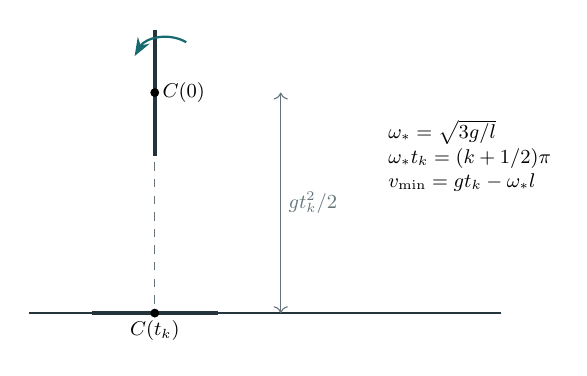
\begin{tikzpicture}[scale=.8,transform shape]

\draw[object] (-2,-3.5)--(5.5,-3.5);
\draw[guide] (0,1)--(0,-3.5);
\draw[object,line width=1.4pt] (0,1)--(0,-1);
\fill (0,0) circle (2pt) node[right] {$C(0)$};
\draw[object,line width=1.4pt] (-1,-3.5)--(1,-3.5);
\fill (0,-3.5) circle (2pt) node[below] {$C(t_k)$};
\draw[axis,<->] (2,0)--(2,-3.5) node[midway,right] {$gt_k^2/2$};
\draw[motion] (.5,.8) arc[start angle=60,end angle=150,radius=.6];
\node[align=left] at (5,-1) {$\omega_*=\sqrt{3g/l}$\\$\omega_*t_k=(k+1/2)\pi$\\$v_{\min}=gt_k-\omega_*l$};

\end{tikzpicture}
\figcaption{解图综四.3C\quad 自由落体质心与匀速转动叠加；各点向下速度和此前最低高度共同确定可行的水平时刻。}
\end{minipage}\end{center}
解图综四.3C以脱梁为$t=0$，用$z_C$表示质心距地高度。此时
\[
z_C=h-l-\frac12gt^2.
\]
以脱梁时指向上端的杆内坐标记作$\zeta$，$-l\leqslant\zeta\leqslant l$，任一点的高度为$z_\zeta=z_C+\zeta\cos(\omega_*t)$。要让一整段杆在同一时刻都位于地面，系数$\cos(\omega_*t)$为零，同时$z_C=0$。这就是杆水平且质心到地面的两个条件，因而候选时刻满足
\[
s_k=\omega_*t_k=\left(k+\frac12\right)\pi,\quad k=0,1,2,\ldots,
\]
\[
h=l+\frac12gt_k^2
=\left[1+\frac{\pi^2}{6}\left(k+\frac12\right)^2\right]l.
\]
水平条件给出几何候选；再以各点向下速度与此前端点高度选择首次整体接触的时刻。由任意点高度求导，向下速度为$gt+\zeta\omega_*\sin(\omega_*t)$。水平时刻正弦的绝对值为1，在整个杆内取最小值，对应旋转速度指向上的那个端点。因此到$t_k$，所有点竖直速度的最小值为
\[
v_{\min}=gt_k-\omega_*l
=\sqrt{\frac{gl}{3}}(s_k-3).
\]
$k=0$时$s_0=\pi/2<3$，有一端在这个水平时刻向上；这一候选轨迹已经与此前的地面接触发生冲突。其高度$h_0=(1+\pi^2/24)l<2l$还使杆在竖直脱梁时的下端低于地面，说明受约束摆下阶段已会先触地。因此取首次整体向下落地时排除$k=0$。$k\ge1$时所有点向下。
\begin{center}\begin{minipage}{.98\linewidth}\centering
\begin{tikzpicture}[scale=.85,transform shape]

\draw[axis] (0,0)--(6.4,0) node[right] {$s=\omega_*t$};
\draw[axis] (0,0)--(0,4.4) node[above] {$d/l$};
\draw[traj,domain=0:4.712389,samples=220] plot ({1.2*\x},{((4.712389^2-\x^2)/6-abs(cos(deg(\x))))});
\draw[guide] (3.7699,0)--(3.7699,3.3);
\node[below] at (3.7699,0) {$s_1-\pi/2$};
\node[below right] at (5.65487,0) {$s_1$};
\node at (3.5,4.5) {$k=1:\ d>0\ (0\le s<s_1)$};
\node at (2.8,-1.2) {早段质心离地大于$l$；末段用$\sin q\le q$};

\end{tikzpicture}
\figcaption{解图综四.3D\quad 最低端高度包络检查整个飞行，在最后水平时刻才首次为零。}
\end{minipage}\end{center}
解图综四.3D以最低端高度覆盖整个下落过程。记$s=\omega_*t$，则最低端距地
\[
\frac{d(s)}l
=\frac{s_k^2-s^2}{6}-|\cos s|,\qquad 0\le s\le s_k.
\]
在任意角位置，杆的两个端点相对质心的高度为$\pm l\cos s$，其中较低者比质心低$l|\cos s|$；所以这个包络同时包含两端，并在穿过水平时自动交换最低端。对$k\ge1$，若$0\le s\le s_k-\pi/2$，有
\[
\frac{s_k^2-s^2}{6}
\ge\frac{\pi s_k-\pi^2/4}{6}
\ge\frac{5\pi^2}{24}>1,
\]
而$|\cos s|\le1$，故$d>0$。最后四分之一转内，令$q=s_k-s\in(0,\pi/2]$，则$|\cos s|=\sin q$，
\[
\frac dl=\frac{q(2s_k-q)}6-\sin q
\ge\frac{5\pi}{12}q-\sin q
\ge\left(\frac{5\pi}{12}-1\right)q>0.
\]
直到$q=0$才有$d=0$，证明更早没有杆端碰地。

上面最后四分之一转的正高度，还可从时间反演读出一个直接的速度意义。令反演时间为$\tau$，从水平着地状态反向上抛质心，其初速为$gt_k$，杆以同样大小的角速度反转。该段里最慢端点的向上速度为
\[
v_{\rm up,min}(\tau)=gt_k-g\tau-\omega_*l\cos(\omega_*\tau),
\qquad0\leqslant\tau\leqslant\frac{\pi}{2\omega_*}.
\]
用单位$\sqrt{gl/3}$表示，需从$s_k$中减去的量为$\omega_*\tau+3\cos(\omega_*\tau)$。在这段中它至多为$\pi/2+3$，而$k\geqslant1$时$s_k\geqslant3\pi/2>\pi/2+3$。故反演的最慢端点仍向上，正演中这最后一段在最终水平之前保持正高度。解图综四.3E画出$k=1$的实际向上速度和上述正下界。
\begin{center}\begin{minipage}{.98\linewidth}\centering
\begin{tikzpicture}[scale=0.72,transform shape]
\draw[axis] (0,0)--(6.2,0);\draw[axis] (0,0)--(0,3.4000000000000004);
\draw[thin,color=muted] (0.0000000,0)--(0.0000000,-.07);\node[below] at (0.0000000,-.09) {$0$};
\draw[thin,color=muted] (3.0000000,0)--(3.0000000,-.07);\node[below] at (3.0000000,-.09) {$\pi/4$};
\draw[thin,color=muted] (6.0000000,0)--(6.0000000,-.07);\node[below] at (6.0000000,-.09) {$\pi/2$};
\draw[thin,color=muted] (0,0.0000000)--(-.07,0.0000000);\node[left] at (-.09,0.0000000) {$0$};
\draw[thin,color=muted] (0,0.9696970)--(-.07,0.9696970);\node[left] at (-.09,0.9696970) {$1$};
\draw[thin,color=muted] (0,1.9393939)--(-.07,1.9393939);\node[left] at (-.09,1.9393939) {$2$};
\draw[thin,color=muted] (0,2.9090909)--(-.07,2.9090909);\node[left] at (-.09,2.9090909) {$3$};
\node[below] at (3.0,-.64) {反演角时间$q=\omega_*\tau$};\node[above right] at (0,3.45) {速度除以$\sqrt{gl/3}$};
\draw[traj] plot coordinates {(0.0000000,1.6604984) (0.0200000,1.6554610) (0.0400000,1.6505033) (0.0600000,1.6456253) (0.0800000,1.6408271) (0.1000000,1.6361087) (0.1200000,1.6314699) (0.1400000,1.6269109) (0.1600000,1.6224316) (0.1800000,1.6180320) (0.2000000,1.6137120) (0.2200000,1.6094717) (0.2400000,1.6053110) (0.2600000,1.6012299) (0.2800000,1.5972283) (0.3000000,1.5933063) (0.3200000,1.5894639) (0.3400000,1.5857008) (0.3600000,1.5820173) (0.3800000,1.5784131) (0.4000000,1.5748883) (0.4200000,1.5714428) (0.4400000,1.5680766) (0.4600000,1.5647896) (0.4800000,1.5615817) (0.5000000,1.5584530) (0.5200000,1.5554034) (0.5400000,1.5524328) (0.5600000,1.5495412) (0.5800000,1.5467284) (0.6000000,1.5439945) (0.6200000,1.5413394) (0.6400000,1.5387629) (0.6600000,1.5362651) (0.6800000,1.5338459) (0.7000000,1.5315052) (0.7200000,1.5292428) (0.7400000,1.5270589) (0.7600000,1.5249531) (0.7800000,1.5229256) (0.8000000,1.5209762) (0.8200000,1.5191047) (0.8400000,1.5173112) (0.8600000,1.5155956) (0.8800000,1.5139576) (0.9000000,1.5123974) (0.9200000,1.5109146) (0.9400000,1.5095093) (0.9600000,1.5081814) (0.9800000,1.5069307) (1.0000000,1.5057572) (1.0200000,1.5046607) (1.0400000,1.5036411) (1.0600000,1.5026984) (1.0800000,1.5018323) (1.1000000,1.5010429) (1.1200000,1.5003299) (1.1400000,1.4996932) (1.1600000,1.4991328) (1.1800000,1.4986485) (1.2000000,1.4982402) (1.2200000,1.4979077) (1.2400000,1.4976509) (1.2600000,1.4974697) (1.2800000,1.4973640) (1.3000000,1.4973336) (1.3200000,1.4973784) (1.3400000,1.4974982) (1.3600000,1.4976929) (1.3800000,1.4979624) (1.4000000,1.4983065) (1.4200000,1.4987250) (1.4400000,1.4992178) (1.4600000,1.4997848) (1.4800000,1.5004258) (1.5000000,1.5011407) (1.5200000,1.5019292) (1.5400000,1.5027912) (1.5600000,1.5037266) (1.5800000,1.5047352) (1.6000000,1.5058168) (1.6200000,1.5069713) (1.6400000,1.5081985) (1.6600000,1.5094981) (1.6800000,1.5108702) (1.7000000,1.5123143) (1.7200000,1.5138305) (1.7400000,1.5154185) (1.7600000,1.5170781) (1.7800000,1.5188091) (1.8000000,1.5206114) (1.8200000,1.5224847) (1.8400000,1.5244290) (1.8600000,1.5264439) (1.8800000,1.5285292) (1.9000000,1.5306849) (1.9200000,1.5329107) (1.9400000,1.5352063) (1.9600000,1.5375716) (1.9800000,1.5400064) (2.0000000,1.5425105) (2.0200000,1.5450837) (2.0400000,1.5477257) (2.0600000,1.5504364) (2.0800000,1.5532155) (2.1000000,1.5560628) (2.1200000,1.5589781) (2.1400000,1.5619612) (2.1600000,1.5650119) (2.1800000,1.5681299) (2.2000000,1.5713150) (2.2200000,1.5745670) (2.2400000,1.5778857) (2.2600000,1.5812708) (2.2800000,1.5847221) (2.3000000,1.5882393) (2.3200000,1.5918223) (2.3400000,1.5954708) (2.3600000,1.5991845) (2.3800000,1.6029633) (2.4000000,1.6068068) (2.4200000,1.6107148) (2.4400000,1.6146871) (2.4600000,1.6187234) (2.4800000,1.6228235) (2.5000000,1.6269871) (2.5200000,1.6312140) (2.5400000,1.6355040) (2.5600000,1.6398567) (2.5800000,1.6442718) (2.6000000,1.6487493) (2.6200000,1.6532887) (2.6400000,1.6578898) (2.6600000,1.6625524) (2.6800000,1.6672762) (2.7000000,1.6720608) (2.7200000,1.6769062) (2.7400000,1.6818119) (2.7600000,1.6867777) (2.7800000,1.6918033) (2.8000000,1.6968885) (2.8200000,1.7020329) (2.8400000,1.7072363) (2.8600000,1.7124985) (2.8800000,1.7178190) (2.9000000,1.7231977) (2.9200000,1.7286343) (2.9400000,1.7341284) (2.9600000,1.7396798) (2.9800000,1.7452881) (3.0000000,1.7509532) (3.0200000,1.7566746) (3.0400000,1.7624522) (3.0600000,1.7682855) (3.0800000,1.7741744) (3.1000000,1.7801184) (3.1200000,1.7861174) (3.1400000,1.7921710) (3.1600000,1.7982788) (3.1800000,1.8044406) (3.2000000,1.8106561) (3.2200000,1.8169250) (3.2400000,1.8232469) (3.2600000,1.8296216) (3.2800000,1.8360487) (3.3000000,1.8425279) (3.3200000,1.8490589) (3.3400000,1.8556413) (3.3600000,1.8622750) (3.3800000,1.8689594) (3.4000000,1.8756944) (3.4200000,1.8824796) (3.4400000,1.8893147) (3.4600000,1.8961992) (3.4800000,1.9031330) (3.5000000,1.9101157) (3.5200000,1.9171469) (3.5400000,1.9242264) (3.5600000,1.9313537) (3.5800000,1.9385286) (3.6000000,1.9457507) (3.6200000,1.9530197) (3.6400000,1.9603352) (3.6600000,1.9676969) (3.6800000,1.9751045) (3.7000000,1.9825576) (3.7200000,1.9900559) (3.7400000,1.9975990) (3.7600000,2.0051866) (3.7800000,2.0128183) (3.8000000,2.0204938) (3.8200000,2.0282127) (3.8400000,2.0359747) (3.8600000,2.0437795) (3.8800000,2.0516266) (3.9000000,2.0595158) (3.9200000,2.0674466) (3.9400000,2.0754188) (3.9600000,2.0834319) (3.9800000,2.0914856) (4.0000000,2.0995796) (4.0200000,2.1077134) (4.0400000,2.1158867) (4.0600000,2.1240992) (4.0800000,2.1323505) (4.1000000,2.1406402) (4.1200000,2.1489680) (4.1400000,2.1573334) (4.1600000,2.1657362) (4.1800000,2.1741759) (4.2000000,2.1826522) (4.2200000,2.1911647) (4.2400000,2.1997130) (4.2600000,2.2082968) (4.2800000,2.2169157) (4.3000000,2.2255693) (4.3200000,2.2342572) (4.3400000,2.2429791) (4.3600000,2.2517346) (4.3800000,2.2605232) (4.4000000,2.2693447) (4.4200000,2.2781986) (4.4400000,2.2870846) (4.4600000,2.2960023) (4.4800000,2.3049512) (4.5000000,2.3139311) (4.5200000,2.3229415) (4.5400000,2.3319820) (4.5600000,2.3410522) (4.5800000,2.3501518) (4.6000000,2.3592804) (4.6200000,2.3684376) (4.6400000,2.3776230) (4.6600000,2.3868361) (4.6800000,2.3960767) (4.7000000,2.4053443) (4.7200000,2.4146385) (4.7400000,2.4239589) (4.7600000,2.4333052) (4.7800000,2.4426769) (4.8000000,2.4520736) (4.8200000,2.4614950) (4.8400000,2.4709407) (4.8600000,2.4804102) (4.8800000,2.4899031) (4.9000000,2.4994191) (4.9200000,2.5089577) (4.9400000,2.5185186) (4.9600000,2.5281014) (4.9800000,2.5377056) (5.0000000,2.5473308) (5.0200000,2.5569767) (5.0400000,2.5666428) (5.0600000,2.5763288) (5.0800000,2.5860342) (5.1000000,2.5957586) (5.1200000,2.6055016) (5.1400000,2.6152628) (5.1600000,2.6250419) (5.1800000,2.6348383) (5.2000000,2.6446517) (5.2200000,2.6544817) (5.2400000,2.6643279) (5.2600000,2.6741899) (5.2800000,2.6840672) (5.3000000,2.6939594) (5.3200000,2.7038662) (5.3400000,2.7137871) (5.3600000,2.7237217) (5.3800000,2.7336696) (5.4000000,2.7436304) (5.4200000,2.7536037) (5.4400000,2.7635891) (5.4600000,2.7735861) (5.4800000,2.7835943) (5.5000000,2.7936134) (5.5200000,2.8036428) (5.5400000,2.8136823) (5.5600000,2.8237313) (5.5800000,2.8337895) (5.6000000,2.8438565) (5.6200000,2.8539318) (5.6400000,2.8640150) (5.6600000,2.8741058) (5.6800000,2.8842036) (5.7000000,2.8943081) (5.7200000,2.9044188) (5.7400000,2.9145354) (5.7600000,2.9246574) (5.7800000,2.9347844) (5.8000000,2.9449160) (5.8200000,2.9550518) (5.8400000,2.9651914) (5.8600000,2.9753342) (5.8800000,2.9854801) (5.9000000,2.9956284) (5.9200000,3.0057788) (5.9400000,3.0159308) (5.9600000,3.0260841) (5.9800000,3.0362383) (6.0000000,3.0463929)};
\draw[traj] (.1,-1.05)--(.7,-1.05);\node[right] at (.85,-1.05) {最慢端点实际向上速度};\draw[dashed,thick,color=warm] plot coordinates {(0.0000000,0.1373020) (0.0200000,0.1373020) (0.0400000,0.1373020) (0.0600000,0.1373020) (0.0800000,0.1373020) (0.1000000,0.1373020) (0.1200000,0.1373020) (0.1400000,0.1373020) (0.1600000,0.1373020) (0.1800000,0.1373020) (0.2000000,0.1373020) (0.2200000,0.1373020) (0.2400000,0.1373020) (0.2600000,0.1373020) (0.2800000,0.1373020) (0.3000000,0.1373020) (0.3200000,0.1373020) (0.3400000,0.1373020) (0.3600000,0.1373020) (0.3800000,0.1373020) (0.4000000,0.1373020) (0.4200000,0.1373020) (0.4400000,0.1373020) (0.4600000,0.1373020) (0.4800000,0.1373020) (0.5000000,0.1373020) (0.5200000,0.1373020) (0.5400000,0.1373020) (0.5600000,0.1373020) (0.5800000,0.1373020) (0.6000000,0.1373020) (0.6200000,0.1373020) (0.6400000,0.1373020) (0.6600000,0.1373020) (0.6800000,0.1373020) (0.7000000,0.1373020) (0.7200000,0.1373020) (0.7400000,0.1373020) (0.7600000,0.1373020) (0.7800000,0.1373020) (0.8000000,0.1373020) (0.8200000,0.1373020) (0.8400000,0.1373020) (0.8600000,0.1373020) (0.8800000,0.1373020) (0.9000000,0.1373020) (0.9200000,0.1373020) (0.9400000,0.1373020) (0.9600000,0.1373020) (0.9800000,0.1373020) (1.0000000,0.1373020) (1.0200000,0.1373020) (1.0400000,0.1373020) (1.0600000,0.1373020) (1.0800000,0.1373020) (1.1000000,0.1373020) (1.1200000,0.1373020) (1.1400000,0.1373020) (1.1600000,0.1373020) (1.1800000,0.1373020) (1.2000000,0.1373020) (1.2200000,0.1373020) (1.2400000,0.1373020) (1.2600000,0.1373020) (1.2800000,0.1373020) (1.3000000,0.1373020) (1.3200000,0.1373020) (1.3400000,0.1373020) (1.3600000,0.1373020) (1.3800000,0.1373020) (1.4000000,0.1373020) (1.4200000,0.1373020) (1.4400000,0.1373020) (1.4600000,0.1373020) (1.4800000,0.1373020) (1.5000000,0.1373020) (1.5200000,0.1373020) (1.5400000,0.1373020) (1.5600000,0.1373020) (1.5800000,0.1373020) (1.6000000,0.1373020) (1.6200000,0.1373020) (1.6400000,0.1373020) (1.6600000,0.1373020) (1.6800000,0.1373020) (1.7000000,0.1373020) (1.7200000,0.1373020) (1.7400000,0.1373020) (1.7600000,0.1373020) (1.7800000,0.1373020) (1.8000000,0.1373020) (1.8200000,0.1373020) (1.8400000,0.1373020) (1.8600000,0.1373020) (1.8800000,0.1373020) (1.9000000,0.1373020) (1.9200000,0.1373020) (1.9400000,0.1373020) (1.9600000,0.1373020) (1.9800000,0.1373020) (2.0000000,0.1373020) (2.0200000,0.1373020) (2.0400000,0.1373020) (2.0600000,0.1373020) (2.0800000,0.1373020) (2.1000000,0.1373020) (2.1200000,0.1373020) (2.1400000,0.1373020) (2.1600000,0.1373020) (2.1800000,0.1373020) (2.2000000,0.1373020) (2.2200000,0.1373020) (2.2400000,0.1373020) (2.2600000,0.1373020) (2.2800000,0.1373020) (2.3000000,0.1373020) (2.3200000,0.1373020) (2.3400000,0.1373020) (2.3600000,0.1373020) (2.3800000,0.1373020) (2.4000000,0.1373020) (2.4200000,0.1373020) (2.4400000,0.1373020) (2.4600000,0.1373020) (2.4800000,0.1373020) (2.5000000,0.1373020) (2.5200000,0.1373020) (2.5400000,0.1373020) (2.5600000,0.1373020) (2.5800000,0.1373020) (2.6000000,0.1373020) (2.6200000,0.1373020) (2.6400000,0.1373020) (2.6600000,0.1373020) (2.6800000,0.1373020) (2.7000000,0.1373020) (2.7200000,0.1373020) (2.7400000,0.1373020) (2.7600000,0.1373020) (2.7800000,0.1373020) (2.8000000,0.1373020) (2.8200000,0.1373020) (2.8400000,0.1373020) (2.8600000,0.1373020) (2.8800000,0.1373020) (2.9000000,0.1373020) (2.9200000,0.1373020) (2.9400000,0.1373020) (2.9600000,0.1373020) (2.9800000,0.1373020) (3.0000000,0.1373020) (3.0200000,0.1373020) (3.0400000,0.1373020) (3.0600000,0.1373020) (3.0800000,0.1373020) (3.1000000,0.1373020) (3.1200000,0.1373020) (3.1400000,0.1373020) (3.1600000,0.1373020) (3.1800000,0.1373020) (3.2000000,0.1373020) (3.2200000,0.1373020) (3.2400000,0.1373020) (3.2600000,0.1373020) (3.2800000,0.1373020) (3.3000000,0.1373020) (3.3200000,0.1373020) (3.3400000,0.1373020) (3.3600000,0.1373020) (3.3800000,0.1373020) (3.4000000,0.1373020) (3.4200000,0.1373020) (3.4400000,0.1373020) (3.4600000,0.1373020) (3.4800000,0.1373020) (3.5000000,0.1373020) (3.5200000,0.1373020) (3.5400000,0.1373020) (3.5600000,0.1373020) (3.5800000,0.1373020) (3.6000000,0.1373020) (3.6200000,0.1373020) (3.6400000,0.1373020) (3.6600000,0.1373020) (3.6800000,0.1373020) (3.7000000,0.1373020) (3.7200000,0.1373020) (3.7400000,0.1373020) (3.7600000,0.1373020) (3.7800000,0.1373020) (3.8000000,0.1373020) (3.8200000,0.1373020) (3.8400000,0.1373020) (3.8600000,0.1373020) (3.8800000,0.1373020) (3.9000000,0.1373020) (3.9200000,0.1373020) (3.9400000,0.1373020) (3.9600000,0.1373020) (3.9800000,0.1373020) (4.0000000,0.1373020) (4.0200000,0.1373020) (4.0400000,0.1373020) (4.0600000,0.1373020) (4.0800000,0.1373020) (4.1000000,0.1373020) (4.1200000,0.1373020) (4.1400000,0.1373020) (4.1600000,0.1373020) (4.1800000,0.1373020) (4.2000000,0.1373020) (4.2200000,0.1373020) (4.2400000,0.1373020) (4.2600000,0.1373020) (4.2800000,0.1373020) (4.3000000,0.1373020) (4.3200000,0.1373020) (4.3400000,0.1373020) (4.3600000,0.1373020) (4.3800000,0.1373020) (4.4000000,0.1373020) (4.4200000,0.1373020) (4.4400000,0.1373020) (4.4600000,0.1373020) (4.4800000,0.1373020) (4.5000000,0.1373020) (4.5200000,0.1373020) (4.5400000,0.1373020) (4.5600000,0.1373020) (4.5800000,0.1373020) (4.6000000,0.1373020) (4.6200000,0.1373020) (4.6400000,0.1373020) (4.6600000,0.1373020) (4.6800000,0.1373020) (4.7000000,0.1373020) (4.7200000,0.1373020) (4.7400000,0.1373020) (4.7600000,0.1373020) (4.7800000,0.1373020) (4.8000000,0.1373020) (4.8200000,0.1373020) (4.8400000,0.1373020) (4.8600000,0.1373020) (4.8800000,0.1373020) (4.9000000,0.1373020) (4.9200000,0.1373020) (4.9400000,0.1373020) (4.9600000,0.1373020) (4.9800000,0.1373020) (5.0000000,0.1373020) (5.0200000,0.1373020) (5.0400000,0.1373020) (5.0600000,0.1373020) (5.0800000,0.1373020) (5.1000000,0.1373020) (5.1200000,0.1373020) (5.1400000,0.1373020) (5.1600000,0.1373020) (5.1800000,0.1373020) (5.2000000,0.1373020) (5.2200000,0.1373020) (5.2400000,0.1373020) (5.2600000,0.1373020) (5.2800000,0.1373020) (5.3000000,0.1373020) (5.3200000,0.1373020) (5.3400000,0.1373020) (5.3600000,0.1373020) (5.3800000,0.1373020) (5.4000000,0.1373020) (5.4200000,0.1373020) (5.4400000,0.1373020) (5.4600000,0.1373020) (5.4800000,0.1373020) (5.5000000,0.1373020) (5.5200000,0.1373020) (5.5400000,0.1373020) (5.5600000,0.1373020) (5.5800000,0.1373020) (5.6000000,0.1373020) (5.6200000,0.1373020) (5.6400000,0.1373020) (5.6600000,0.1373020) (5.6800000,0.1373020) (5.7000000,0.1373020) (5.7200000,0.1373020) (5.7400000,0.1373020) (5.7600000,0.1373020) (5.7800000,0.1373020) (5.8000000,0.1373020) (5.8200000,0.1373020) (5.8400000,0.1373020) (5.8600000,0.1373020) (5.8800000,0.1373020) (5.9000000,0.1373020) (5.9200000,0.1373020) (5.9400000,0.1373020) (5.9600000,0.1373020) (5.9800000,0.1373020) (6.0000000,0.1373020)};
\draw[dashed,thick,color=warm] (.1,-1.48)--(.7,-1.48);\node[right] at (.85,-1.48) {统一正下界};\end{tikzpicture}
\figcaption{解图综四.3E\quad k等于1时反演的最慢端点仍上升，正演末段在最终水平前保持分离}
\end{minipage}\end{center}
最终允许的横梁高度是
\[
\boxed{h=\left[1+\frac{\pi^2}{6}\left(k+\frac12\right)^2\right]l,\qquad k=1,2,\ldots}.
\]
最小值为$h_{\min}=(1+3\pi^2/8)l\simeq4.70l$。这个高度也大于$2l$，因此脱梁前的整个摆下阶段，杆的下端高度$h-2l\cos\phi\geqslant h-2l>0$，与地面保持分离。允许高度的离散性由匀速转动的水平时刻与质心的二次下落位移共同确定；质量在重力势能和惯量中同时约去，所以高度比$h/l$与杆质量无关。完整条件由水平几何、全杆向下速度和全程正高度共同组成，因而选出$k=1,2,\ldots$这一离散高度族。


\Needspace{13\baselineskip}

\pdfbookmark[2]{第 4 题 环形轨道上的连续喷珠与回收}{q4}

\section*{第 4 题\quad 环形轨道上的连续喷珠与回收}\label{q:4}


光滑水平面上固定一个光滑大圆环，半径$R$。一个尺寸可忽略的发射装置$P$紧贴环内侧，起初静止，其头朝右、尾朝左。装置干质量为$m$，内部许多光滑微珠的总质量也为$m$。

从$t=0$起，装置从尾部沿切线向后连续发珠，珠相对装置的喷出速率恒为$u$，质量流率恒定。当装置的头首次与沿环逆行、从前方迎来的珠相遇时，恰好全部珠已发完，记此时为$T$。

（1）求发射全过程装置相对圆环转过的角度，精确到$1^\circ$。（2）若此后装置把迎来的珠吞入，不再发射，求最终速率，并证明所有珠都能被回收。忽略装置和微珠在轨道上的尺寸以及珠间相互碰撞。


\begin{center}\begin{minipage}{.98\linewidth}\centering
\begin{tikzpicture}[scale=.85,transform shape]

\draw[object] (0,0) circle (2);
\fill[accent] (-.3,1.88) rectangle (.3,2.12);
\node[above] at (0,2.2) {$P$};
\draw[motion] (.4,2)--(1.3,2) node[right] {$v$正向};
\draw[motion] (-.4,2)--(-1.3,2) node[left] {喷珠};
\fill (0,0) circle (2pt) node[below] {$O$};
\draw[guide] (0,0)--(1.414,-1.414) node[midway,below left] {$R$};

\node[align=left] at (5,0) {干质量$m$\\待发珠总质量$m$\\相对喷速$u$};

\end{tikzpicture}
\figcaption{图综四.4\quad 以装置初始头向为沿环正向；支持力对环心无力矩。}
\end{minipage}\end{center}

\Needspace{6\baselineskip}\subsection*{解答}


图综四.4把装置初始头向规定为沿环正向。圆环支持力沿径向，对环心无力矩；包括装置、待发珠和已发珠的整个系统关于环心的总角动量守恒，初值为零。运动沿途的切线方向在变；圆环给系统径向冲量，而对环心不产生力矩。
\begin{center}\begin{minipage}{.98\linewidth}\centering
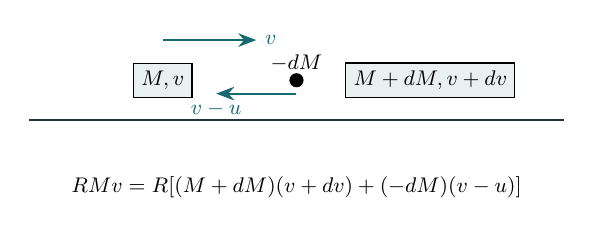
\begin{tikzpicture}[scale=.85,transform shape]

\draw[object] (-2,0)--(6,0);
\node[draw,fill=accent!10] at (0,.6) {$M,v$};
\draw[motion] (0,1.2)--(1.4,1.2) node[right] {$v$};
\node[draw,fill=accent!10] at (4,.6) {$M+dM,v+dv$};
\fill (2,.6) circle (3pt) node[above] {$-dM$};
\draw[motion] (2,.4)--(.8,.4) node[below] {$v-u$};
\node at (2,-1) {$RMv=R[(M+dM)(v+dv)+(-dM)(v-u)]$};

\end{tikzpicture}
\figcaption{解图综四.4A\quad 局部切向发射微元，但守恒式使用关于同一环心的角动量。}
\end{minipage}\end{center}
解图综四.4A取一个极短发射过程。装置连同待发珠的瞬时质量为$M$、正向速率为$v$，射出珠质量$-dM>0$；到一阶，珠相对圆环的有向速度为$v-u$。发射前后关于环心的角动量守恒：
\[
RMv=R[(M+dM)(v+dv)+(-dM)(v-u)].
\]
略去二阶小量$dM\,dv$，得到
\[
M\,dv+u\,dM=0,\qquad
dv=-u\frac{dM}{M}.
\]
若质量流率为$\mu$，则$\mu T=m$，且
$M(t)=2m-\mu t$。从$M(0)=2m,v(0)=0$积分，
\[
\boxed{v(t)=u\ln\frac{2m}{2m-\mu t}},\qquad 0\le t\le T.
\]
因而末速$v(T)=u\ln2<u$；所有发出的珠都逆着装置的正方向运动，速率在$u(1-\ln2)$与$u$之间。
\begin{center}\begin{minipage}{.98\linewidth}\centering
\begin{tikzpicture}[scale=.85,transform shape]

\draw[axis] (0,0)--(6,0) node[right] {$t/T$};
\draw[axis] (0,0)--(0,3.5) node[above] {弧长$/uT$};
\draw[traj,domain=0:1,samples=100] plot ({5*\x},{3*(\x+(2-\x)*ln(1-\x/2))});
\draw[object] (0,0)--(5,3) node[right] {$\ell_0/uT=t/T$};
\draw[guide] (5,0)--(5,3);
\node[below] at (5,0) {$1$};
\node[above left] at (5,.92056) {$\ell_P/uT=1-\ln2$};
\node at (3,-1.3) {$\ell_P(T)+\ell_0(T)=2\pi R$};

\end{tikzpicture}
\figcaption{解图综四.4B\quad 装置弧长由变速积分得到，第一珠逆向弧长随时间线性增长。}
\end{minipage}\end{center}
解图综四.4B以展开的圆周弧长记录两种运动。装置发射期间的路程为
\[
\ell_P=\int_0^T v(t)dt
=\frac u\mu\int_m^{2m}\ln\frac{2m}{M}\,dM.
\]
被积函数的原函数是$M[\ln(2m/M)+1]$，因此
\[
\ell_P=\frac u\mu\{2m-m(1+\ln2)\}
=\boxed{uT(1-\ln2)}.
\]
第一颗珠在$t=0$发出，装置初速零，故珠以逆向恒速$u$运动，至$T$的路程为$\ell_0=uT$。
题设首次迎头相遇对应两者相向走完一周：
\[
\ell_P+\ell_0=uT(2-\ln2)=2\pi R.
\]
故装置转角为
\[
\boxed{\theta=\frac{\ell_P}{R}
=2\pi\frac{1-\ln2}{2-\ln2}
=360^\circ\frac{1-\ln2}{2-\ln2}
\simeq85^\circ}.
\]
这里按题设取整到度；装置一直加速，图B在$t=T$处的弧长纵坐标给出实际路程。

确定首次迎头相遇，需要比较先后发出的珠子。对于在$\tau$发出的珠，到$t>\tau$与装置累积的相向弧长为
\[
D(t,\tau)=\ell_P(t)-\ell_P(\tau)
+[u-v(\tau)](t-\tau).
\]
对固定$t$求导：
\[
\frac{\partial D}{\partial\tau}
=-u-v'(\tau)(t-\tau)<0.
\]
所以先发的珠累积闭合路程更大，第一珠先达到$2\pi R$，没有后发珠在$T$前先绕回迎头碰到装置。此处不把珠刚离开尾部的接触算作迎头相遇。
\begin{center}\begin{minipage}{.98\linewidth}\centering
\begin{tikzpicture}[scale=.8,transform shape]

\draw[object] (0,0) circle (2);
\fill[accent] (-.3,1.88) rectangle (.3,2.12);
\node[above] at (0,2.2) {$P$};
\draw[motion] (.4,2)--(1.3,2) node[right] {$v$正向};
\draw[motion] (-.4,2)--(-1.3,2) node[left] {喷珠};
\fill (0,0) circle (2pt) node[below] {$O$};
\draw[guide] (0,0)--(1.414,-1.414) node[midway,below left] {$R$};

\foreach \ang in {15,40,70,110,140,170,200,230,270,300,330}{
\fill[warm] (\ang:1.9) circle (1.4pt);}
\node[align=left] at (5.5,.5) {所有游离珠逆行\\$w_i\ge u(1-\ln2)>0$\\$M_Pv=\sum m_iw_i>0$};
\node at (2,-3) {尚未全部回收时装置保持正行；收完后总角动量零};

\end{tikzpicture}
\figcaption{解图综四.4C\quad 回收阶段的正负角动量；非弹性吞入不守恒机械能。}
\end{minipage}\end{center}
第（2）问，解图综四.4C中$T$后停止发射，珠被装置吞入且不再离开。只要还有游离珠，它们都以非零逆向速率运动，最慢的也有
$w_{\min}=u(1-\ln2)>0$。记尚未吞入各珠质量为$m_i$、逆向速率为$w_i$，装置及已吞珠的总质量为$M_P$。总角动量零给
\[
RM_Pv-R\sum_{\rm free}m_iw_i=0,
\quad
\boxed{v=\frac{\sum_{\rm free}m_iw_i}{M_P}>0}.
\]
因此装置在尚未收完珠时保持正向运动，而每颗未收珠持续逆行，相对闭合速率不小于$w_{\min}$。每颗珠最多再走一个相对圆周就必遇到装置，所以在有限时间内能全部收回。

全部回收后总质量为$2m$，系统只剩同一装置的圆周运动。角动量守恒给
\[
2mR\,v_\infty=0,\qquad \boxed{v_\infty=0}.
\]
吞入是非弹性过程，会耗散动能。末态由关于环心的角动量确定，吞入中损失的动能转为内能。

\textbf{发射与回收的完整时间图像。} 解图综四.4D以$x=t/T$为横坐标，将装置与各批珠子的运动画在同一圆周展开坐标中。质量微元$\mu\,dt$离开后，在光滑圆环上只受径向支持力，因此其关于环心的角动量$R\,dm\,w$保持不变，圆环参考系中的有向切向速度$w=v(\tau)-u$也保持不变。珠子的切线方向虽随位置转动，每颗珠子的有向弧长仍随时间线性变化；这正是展开图中各条珠子轨迹为直线的理由。
\begin{center}\begin{minipage}{.98\linewidth}\centering
\begin{tikzpicture}[scale=0.72,transform shape]
\draw[axis] (0,0)--(6.2,0);\draw[axis] (0,0)--(0,3.4000000000000004);
\draw[thin,color=muted] (0.0000000,0)--(0.0000000,-.07);\node[below] at (0.0000000,-.09) {$0$};
\draw[thin,color=muted] (3.0000000,0)--(3.0000000,-.07);\node[below] at (3.0000000,-.09) {$.5$};
\draw[thin,color=muted] (6.0000000,0)--(6.0000000,-.07);\node[below] at (6.0000000,-.09) {$1$};
\draw[thin,color=muted] (0,0.1142857)--(-.07,0.1142857);\node[left] at (-.09,0.1142857) {$-1$};
\draw[thin,color=muted] (0,2.4000000)--(-.07,2.4000000);\node[left] at (-.09,2.4000000) {$0$};
\draw[thin,color=muted] (0,3.0857143)--(-.07,3.0857143);\node[left] at (-.09,3.0857143) {$.3$};
\node[below] at (3.0,-.64) {$t/T$};\node[above right] at (0,3.45) {有向弧长除以uT};
\draw[traj] plot coordinates {(0.0000000,2.4000000) (0.0250000,2.4000099) (0.0500000,2.4000397) (0.0750000,2.4000895) (0.1000000,2.4001592) (0.1250000,2.4002489) (0.1500000,2.4003586) (0.1750000,2.4004885) (0.2000000,2.4006385) (0.2250000,2.4008086) (0.2500000,2.4009990) (0.2750000,2.4012097) (0.3000000,2.4014406) (0.3250000,2.4016919) (0.3500000,2.4019636) (0.3750000,2.4022558) (0.4000000,2.4025684) (0.4250000,2.4029015) (0.4500000,2.4032552) (0.4750000,2.4036296) (0.5000000,2.4040245) (0.5250000,2.4044402) (0.5500000,2.4048767) (0.5750000,2.4053339) (0.6000000,2.4058120) (0.6250000,2.4063109) (0.6500000,2.4068308) (0.6750000,2.4073717) (0.7000000,2.4079336) (0.7250000,2.4085165) (0.7500000,2.4091206) (0.7750000,2.4097459) (0.8000000,2.4103923) (0.8250000,2.4110600) (0.8500000,2.4117491) (0.8750000,2.4124594) (0.9000000,2.4131912) (0.9250000,2.4139444) (0.9500000,2.4147191) (0.9750000,2.4155154) (1.0000000,2.4163333) (1.0250000,2.4171728) (1.0500000,2.4180340) (1.0750000,2.4189169) (1.1000000,2.4198217) (1.1250000,2.4207483) (1.1500000,2.4216967) (1.1750000,2.4226672) (1.2000000,2.4236596) (1.2250000,2.4246741) (1.2500000,2.4257106) (1.2750000,2.4267693) (1.3000000,2.4278502) (1.3250000,2.4289534) (1.3500000,2.4300789) (1.3750000,2.4312267) (1.4000000,2.4323969) (1.4250000,2.4335896) (1.4500000,2.4348048) (1.4750000,2.4360426) (1.5000000,2.4373030) (1.5250000,2.4385861) (1.5500000,2.4398919) (1.5750000,2.4412205) (1.6000000,2.4425719) (1.6250000,2.4439462) (1.6500000,2.4453435) (1.6750000,2.4467638) (1.7000000,2.4482071) (1.7250000,2.4496735) (1.7500000,2.4511632) (1.7750000,2.4526760) (1.8000000,2.4542122) (1.8250000,2.4557716) (1.8500000,2.4573545) (1.8750000,2.4589609) (1.9000000,2.4605907) (1.9250000,2.4622441) (1.9500000,2.4639212) (1.9750000,2.4656219) (2.0000000,2.4673465) (2.0250000,2.4690948) (2.0500000,2.4708669) (2.0750000,2.4726630) (2.1000000,2.4744831) (2.1250000,2.4763273) (2.1500000,2.4781956) (2.1750000,2.4800880) (2.2000000,2.4820047) (2.2250000,2.4839456) (2.2500000,2.4859109) (2.2750000,2.4879007) (2.3000000,2.4899149) (2.3250000,2.4919537) (2.3500000,2.4940170) (2.3750000,2.4961051) (2.4000000,2.4982179) (2.4250000,2.5003555) (2.4500000,2.5025179) (2.4750000,2.5047053) (2.5000000,2.5069177) (2.5250000,2.5091551) (2.5500000,2.5114177) (2.5750000,2.5137055) (2.6000000,2.5160185) (2.6250000,2.5183569) (2.6500000,2.5207206) (2.6750000,2.5231098) (2.7000000,2.5255246) (2.7250000,2.5279650) (2.7500000,2.5304310) (2.7750000,2.5329228) (2.8000000,2.5354403) (2.8250000,2.5379838) (2.8500000,2.5405532) (2.8750000,2.5431486) (2.9000000,2.5457702) (2.9250000,2.5484178) (2.9500000,2.5510918) (2.9750000,2.5537920) (3.0000000,2.5565186) (3.0250000,2.5592717) (3.0500000,2.5620513) (3.0750000,2.5648575) (3.1000000,2.5676904) (3.1250000,2.5705500) (3.1500000,2.5734364) (3.1750000,2.5763498) (3.2000000,2.5792901) (3.2250000,2.5822575) (3.2500000,2.5852521) (3.2750000,2.5882738) (3.3000000,2.5913228) (3.3250000,2.5943992) (3.3500000,2.5975031) (3.3750000,2.6006345) (3.4000000,2.6037934) (3.4250000,2.6069801) (3.4500000,2.6101945) (3.4750000,2.6134368) (3.5000000,2.6167070) (3.5250000,2.6200052) (3.5500000,2.6233315) (3.5750000,2.6266860) (3.6000000,2.6300688) (3.6250000,2.6334798) (3.6500000,2.6369194) (3.6750000,2.6403874) (3.7000000,2.6438840) (3.7250000,2.6474094) (3.7500000,2.6509634) (3.7750000,2.6545464) (3.8000000,2.6581583) (3.8250000,2.6617992) (3.8500000,2.6654693) (3.8750000,2.6691686) (3.9000000,2.6728972) (3.9250000,2.6766551) (3.9500000,2.6804426) (3.9750000,2.6842596) (4.0000000,2.6881063) (4.0250000,2.6919828) (4.0500000,2.6958891) (4.0750000,2.6998254) (4.1000000,2.7037917) (4.1250000,2.7077882) (4.1500000,2.7118149) (4.1750000,2.7158719) (4.2000000,2.7199593) (4.2250000,2.7240773) (4.2500000,2.7282259) (4.2750000,2.7324052) (4.3000000,2.7366154) (4.3250000,2.7408564) (4.3500000,2.7451285) (4.3750000,2.7494317) (4.4000000,2.7537661) (4.4250000,2.7581319) (4.4500000,2.7625291) (4.4750000,2.7669578) (4.5000000,2.7714182) (4.5250000,2.7759103) (4.5500000,2.7804343) (4.5750000,2.7849902) (4.6000000,2.7895782) (4.6250000,2.7941984) (4.6500000,2.7988508) (4.6750000,2.8035357) (4.7000000,2.8082530) (4.7250000,2.8130030) (4.7500000,2.8177857) (4.7750000,2.8226012) (4.8000000,2.8274497) (4.8250000,2.8323313) (4.8500000,2.8372460) (4.8750000,2.8421941) (4.9000000,2.8471755) (4.9250000,2.8521905) (4.9500000,2.8572392) (4.9750000,2.8623216) (5.0000000,2.8674379) (5.0250000,2.8725882) (5.0500000,2.8777727) (5.0750000,2.8829914) (5.1000000,2.8882445) (5.1250000,2.8935321) (5.1500000,2.8988544) (5.1750000,2.9042114) (5.2000000,2.9096033) (5.2250000,2.9150302) (5.2500000,2.9204922) (5.2750000,2.9259895) (5.3000000,2.9315222) (5.3250000,2.9370905) (5.3500000,2.9426944) (5.3750000,2.9483342) (5.4000000,2.9540098) (5.4250000,2.9597216) (5.4500000,2.9654695) (5.4750000,2.9712538) (5.5000000,2.9770746) (5.5250000,2.9829321) (5.5500000,2.9888263) (5.5750000,2.9947574) (5.6000000,3.0007256) (5.6250000,3.0067309) (5.6500000,3.0127737) (5.6750000,3.0188539) (5.7000000,3.0249717) (5.7250000,3.0311274) (5.7500000,3.0373210) (5.7750000,3.0435527) (5.8000000,3.0498226) (5.8250000,3.0561310) (5.8500000,3.0624779) (5.8750000,3.0688635) (5.9000000,3.0752880) (5.9250000,3.0817515) (5.9500000,3.0882542) (5.9750000,3.0947963) (6.0000000,3.1013779)};
\draw[traj] (.1,-1.05)--(.7,-1.05);\node[right] at (.85,-1.05) {装置弧长};\draw[dashed,thick,color=warm] plot coordinates {(0.0000000,2.4000000) (0.0400000,2.3847619) (0.0800000,2.3695238) (0.1200000,2.3542857) (0.1600000,2.3390476) (0.2000000,2.3238095) (0.2400000,2.3085714) (0.2800000,2.2933333) (0.3200000,2.2780952) (0.3600000,2.2628571) (0.4000000,2.2476190) (0.4400000,2.2323810) (0.4800000,2.2171429) (0.5200000,2.2019048) (0.5600000,2.1866667) (0.6000000,2.1714286) (0.6400000,2.1561905) (0.6800000,2.1409524) (0.7200000,2.1257143) (0.7600000,2.1104762) (0.8000000,2.0952381) (0.8400000,2.0800000) (0.8800000,2.0647619) (0.9200000,2.0495238) (0.9600000,2.0342857) (1.0000000,2.0190476) (1.0400000,2.0038095) (1.0800000,1.9885714) (1.1200000,1.9733333) (1.1600000,1.9580952) (1.2000000,1.9428571) (1.2400000,1.9276190) (1.2800000,1.9123810) (1.3200000,1.8971429) (1.3600000,1.8819048) (1.4000000,1.8666667) (1.4400000,1.8514286) (1.4800000,1.8361905) (1.5200000,1.8209524) (1.5600000,1.8057143) (1.6000000,1.7904762) (1.6400000,1.7752381) (1.6800000,1.7600000) (1.7200000,1.7447619) (1.7600000,1.7295238) (1.8000000,1.7142857) (1.8400000,1.6990476) (1.8800000,1.6838095) (1.9200000,1.6685714) (1.9600000,1.6533333) (2.0000000,1.6380952) (2.0400000,1.6228571) (2.0800000,1.6076190) (2.1200000,1.5923810) (2.1600000,1.5771429) (2.2000000,1.5619048) (2.2400000,1.5466667) (2.2800000,1.5314286) (2.3200000,1.5161905) (2.3600000,1.5009524) (2.4000000,1.4857143) (2.4400000,1.4704762) (2.4800000,1.4552381) (2.5200000,1.4400000) (2.5600000,1.4247619) (2.6000000,1.4095238) (2.6400000,1.3942857) (2.6800000,1.3790476) (2.7200000,1.3638095) (2.7600000,1.3485714) (2.8000000,1.3333333) (2.8400000,1.3180952) (2.8800000,1.3028571) (2.9200000,1.2876190) (2.9600000,1.2723810) (3.0000000,1.2571429) (3.0400000,1.2419048) (3.0800000,1.2266667) (3.1200000,1.2114286) (3.1600000,1.1961905) (3.2000000,1.1809524) (3.2400000,1.1657143) (3.2800000,1.1504762) (3.3200000,1.1352381) (3.3600000,1.1200000) (3.4000000,1.1047619) (3.4400000,1.0895238) (3.4800000,1.0742857) (3.5200000,1.0590476) (3.5600000,1.0438095) (3.6000000,1.0285714) (3.6400000,1.0133333) (3.6800000,0.9980952) (3.7200000,0.9828571) (3.7600000,0.9676190) (3.8000000,0.9523810) (3.8400000,0.9371429) (3.8800000,0.9219048) (3.9200000,0.9066667) (3.9600000,0.8914286) (4.0000000,0.8761905) (4.0400000,0.8609524) (4.0800000,0.8457143) (4.1200000,0.8304762) (4.1600000,0.8152381) (4.2000000,0.8000000) (4.2400000,0.7847619) (4.2800000,0.7695238) (4.3200000,0.7542857) (4.3600000,0.7390476) (4.4000000,0.7238095) (4.4400000,0.7085714) (4.4800000,0.6933333) (4.5200000,0.6780952) (4.5600000,0.6628571) (4.6000000,0.6476190) (4.6400000,0.6323810) (4.6800000,0.6171429) (4.7200000,0.6019048) (4.7600000,0.5866667) (4.8000000,0.5714286) (4.8400000,0.5561905) (4.8800000,0.5409524) (4.9200000,0.5257143) (4.9600000,0.5104762) (5.0000000,0.4952381) (5.0400000,0.4800000) (5.0800000,0.4647619) (5.1200000,0.4495238) (5.1600000,0.4342857) (5.2000000,0.4190476) (5.2400000,0.4038095) (5.2800000,0.3885714) (5.3200000,0.3733333) (5.3600000,0.3580952) (5.4000000,0.3428571) (5.4400000,0.3276190) (5.4800000,0.3123810) (5.5200000,0.2971429) (5.5600000,0.2819048) (5.6000000,0.2666667) (5.6400000,0.2514286) (5.6800000,0.2361905) (5.7200000,0.2209524) (5.7600000,0.2057143) (5.8000000,0.1904762) (5.8400000,0.1752381) (5.8800000,0.1600000) (5.9200000,0.1447619) (5.9600000,0.1295238) (6.0000000,0.1142857)};
\draw[dashed,thick,color=warm] (.1,-1.48)--(.7,-1.48);\node[right] at (.85,-1.48) {发射时刻$\tau/T=0$的珠};\draw[dotted,thick,color=muted] plot coordinates {(1.8000000,2.4542122) (1.8280000,2.4452790) (1.8560000,2.4363459) (1.8840000,2.4274128) (1.9120000,2.4184796) (1.9400000,2.4095465) (1.9680000,2.4006134) (1.9960000,2.3916802) (2.0240000,2.3827471) (2.0520000,2.3738140) (2.0800000,2.3648808) (2.1080000,2.3559477) (2.1360000,2.3470146) (2.1640000,2.3380815) (2.1920000,2.3291483) (2.2200000,2.3202152) (2.2480000,2.3112821) (2.2760000,2.3023489) (2.3040000,2.2934158) (2.3320000,2.2844827) (2.3600000,2.2755495) (2.3880000,2.2666164) (2.4160000,2.2576833) (2.4440000,2.2487501) (2.4720000,2.2398170) (2.5000000,2.2308839) (2.5280000,2.2219507) (2.5560000,2.2130176) (2.5840000,2.2040845) (2.6120000,2.1951513) (2.6400000,2.1862182) (2.6680000,2.1772851) (2.6960000,2.1683520) (2.7240000,2.1594188) (2.7520000,2.1504857) (2.7800000,2.1415526) (2.8080000,2.1326194) (2.8360000,2.1236863) (2.8640000,2.1147532) (2.8920000,2.1058200) (2.9200000,2.0968869) (2.9480000,2.0879538) (2.9760000,2.0790206) (3.0040000,2.0700875) (3.0320000,2.0611544) (3.0600000,2.0522212) (3.0880000,2.0432881) (3.1160000,2.0343550) (3.1440000,2.0254219) (3.1720000,2.0164887) (3.2000000,2.0075556) (3.2280000,1.9986225) (3.2560000,1.9896893) (3.2840000,1.9807562) (3.3120000,1.9718231) (3.3400000,1.9628899) (3.3680000,1.9539568) (3.3960000,1.9450237) (3.4240000,1.9360905) (3.4520000,1.9271574) (3.4800000,1.9182243) (3.5080000,1.9092911) (3.5360000,1.9003580) (3.5640000,1.8914249) (3.5920000,1.8824917) (3.6200000,1.8735586) (3.6480000,1.8646255) (3.6760000,1.8556924) (3.7040000,1.8467592) (3.7320000,1.8378261) (3.7600000,1.8288930) (3.7880000,1.8199598) (3.8160000,1.8110267) (3.8440000,1.8020936) (3.8720000,1.7931604) (3.9000000,1.7842273) (3.9280000,1.7752942) (3.9560000,1.7663610) (3.9840000,1.7574279) (4.0120000,1.7484948) (4.0400000,1.7395616) (4.0680000,1.7306285) (4.0960000,1.7216954) (4.1240000,1.7127623) (4.1520000,1.7038291) (4.1800000,1.6948960) (4.2080000,1.6859629) (4.2360000,1.6770297) (4.2640000,1.6680966) (4.2920000,1.6591635) (4.3200000,1.6502303) (4.3480000,1.6412972) (4.3760000,1.6323641) (4.4040000,1.6234309) (4.4320000,1.6144978) (4.4600000,1.6055647) (4.4880000,1.5966315) (4.5160000,1.5876984) (4.5440000,1.5787653) (4.5720000,1.5698321) (4.6000000,1.5608990) (4.6280000,1.5519659) (4.6560000,1.5430328) (4.6840000,1.5340996) (4.7120000,1.5251665) (4.7400000,1.5162334) (4.7680000,1.5073002) (4.7960000,1.4983671) (4.8240000,1.4894340) (4.8520000,1.4805008) (4.8800000,1.4715677) (4.9080000,1.4626346) (4.9360000,1.4537014) (4.9640000,1.4447683) (4.9920000,1.4358352) (5.0200000,1.4269020) (5.0480000,1.4179689) (5.0760000,1.4090358) (5.1040000,1.4001027) (5.1320000,1.3911695) (5.1600000,1.3822364) (5.1880000,1.3733033) (5.2160000,1.3643701) (5.2440000,1.3554370) (5.2720000,1.3465039) (5.3000000,1.3375707) (5.3280000,1.3286376) (5.3560000,1.3197045) (5.3840000,1.3107713) (5.4120000,1.3018382) (5.4400000,1.2929051) (5.4680000,1.2839719) (5.4960000,1.2750388) (5.5240000,1.2661057) (5.5520000,1.2571725) (5.5800000,1.2482394) (5.6080000,1.2393063) (5.6360000,1.2303732) (5.6640000,1.2214400) (5.6920000,1.2125069) (5.7200000,1.2035738) (5.7480000,1.1946406) (5.7760000,1.1857075) (5.8040000,1.1767744) (5.8320000,1.1678412) (5.8600000,1.1589081) (5.8880000,1.1499750) (5.9160000,1.1410418) (5.9440000,1.1321087) (5.9720000,1.1231756) (6.0000000,1.1142424)};
\draw[dotted,thick,color=muted] (.1,-1.9100000000000001)--(.7,-1.9100000000000001);\node[right] at (.85,-1.9100000000000001) {发射时刻$\tau/T=0.3$的珠};\draw[dash dot,thick,color=ink] plot coordinates {(3.9000000,2.6728972) (3.9140000,2.6696601) (3.9280000,2.6664229) (3.9420000,2.6631858) (3.9560000,2.6599487) (3.9700000,2.6567116) (3.9840000,2.6534745) (3.9980000,2.6502374) (4.0120000,2.6470003) (4.0260000,2.6437632) (4.0400000,2.6405261) (4.0540000,2.6372890) (4.0680000,2.6340519) (4.0820000,2.6308148) (4.0960000,2.6275777) (4.1100000,2.6243406) (4.1240000,2.6211035) (4.1380000,2.6178664) (4.1520000,2.6146292) (4.1660000,2.6113921) (4.1800000,2.6081550) (4.1940000,2.6049179) (4.2080000,2.6016808) (4.2220000,2.5984437) (4.2360000,2.5952066) (4.2500000,2.5919695) (4.2640000,2.5887324) (4.2780000,2.5854953) (4.2920000,2.5822582) (4.3060000,2.5790211) (4.3200000,2.5757840) (4.3340000,2.5725469) (4.3480000,2.5693098) (4.3620000,2.5660727) (4.3760000,2.5628355) (4.3900000,2.5595984) (4.4040000,2.5563613) (4.4180000,2.5531242) (4.4320000,2.5498871) (4.4460000,2.5466500) (4.4600000,2.5434129) (4.4740000,2.5401758) (4.4880000,2.5369387) (4.5020000,2.5337016) (4.5160000,2.5304645) (4.5300000,2.5272274) (4.5440000,2.5239903) (4.5580000,2.5207532) (4.5720000,2.5175161) (4.5860000,2.5142790) (4.6000000,2.5110418) (4.6140000,2.5078047) (4.6280000,2.5045676) (4.6420000,2.5013305) (4.6560000,2.4980934) (4.6700000,2.4948563) (4.6840000,2.4916192) (4.6980000,2.4883821) (4.7120000,2.4851450) (4.7260000,2.4819079) (4.7400000,2.4786708) (4.7540000,2.4754337) (4.7680000,2.4721966) (4.7820000,2.4689595) (4.7960000,2.4657224) (4.8100000,2.4624853) (4.8240000,2.4592481) (4.8380000,2.4560110) (4.8520000,2.4527739) (4.8660000,2.4495368) (4.8800000,2.4462997) (4.8940000,2.4430626) (4.9080000,2.4398255) (4.9220000,2.4365884) (4.9360000,2.4333513) (4.9500000,2.4301142) (4.9640000,2.4268771) (4.9780000,2.4236400) (4.9920000,2.4204029) (5.0060000,2.4171658) (5.0200000,2.4139287) (5.0340000,2.4106916) (5.0480000,2.4074544) (5.0620000,2.4042173) (5.0760000,2.4009802) (5.0900000,2.3977431) (5.1040000,2.3945060) (5.1180000,2.3912689) (5.1320000,2.3880318) (5.1460000,2.3847947) (5.1600000,2.3815576) (5.1740000,2.3783205) (5.1880000,2.3750834) (5.2020000,2.3718463) (5.2160000,2.3686092) (5.2300000,2.3653721) (5.2440000,2.3621350) (5.2580000,2.3588979) (5.2720000,2.3556607) (5.2860000,2.3524236) (5.3000000,2.3491865) (5.3140000,2.3459494) (5.3280000,2.3427123) (5.3420000,2.3394752) (5.3560000,2.3362381) (5.3700000,2.3330010) (5.3840000,2.3297639) (5.3980000,2.3265268) (5.4120000,2.3232897) (5.4260000,2.3200526) (5.4400000,2.3168155) (5.4540000,2.3135784) (5.4680000,2.3103413) (5.4820000,2.3071042) (5.4960000,2.3038671) (5.5100000,2.3006299) (5.5240000,2.2973928) (5.5380000,2.2941557) (5.5520000,2.2909186) (5.5660000,2.2876815) (5.5800000,2.2844444) (5.5940000,2.2812073) (5.6080000,2.2779702) (5.6220000,2.2747331) (5.6360000,2.2714960) (5.6500000,2.2682589) (5.6640000,2.2650218) (5.6780000,2.2617847) (5.6920000,2.2585476) (5.7060000,2.2553105) (5.7200000,2.2520734) (5.7340000,2.2488362) (5.7480000,2.2455991) (5.7620000,2.2423620) (5.7760000,2.2391249) (5.7900000,2.2358878) (5.8040000,2.2326507) (5.8180000,2.2294136) (5.8320000,2.2261765) (5.8460000,2.2229394) (5.8600000,2.2197023) (5.8740000,2.2164652) (5.8880000,2.2132281) (5.9020000,2.2099910) (5.9160000,2.2067539) (5.9300000,2.2035168) (5.9440000,2.2002797) (5.9580000,2.1970425) (5.9720000,2.1938054) (5.9860000,2.1905683) (6.0000000,2.1873312)};
\draw[dash dot,thick,color=ink] (.1,-2.34)--(.7,-2.34);\node[right] at (.85,-2.34) {发射时刻$\tau/T=0.65$的珠};\end{tikzpicture}
\figcaption{解图综四.4D\quad 圆周展开后，装置加速前进，各批珠沿不同斜率的直线逆行}
\end{minipage}\end{center}
装置的正向加速度为
\[
\dot v=\frac{u\mu}{2m-\mu t}>0,\qquad
\dot v(0)=\frac{u}{2T},\quad \dot v(T)=\frac uT.
\]
因此其弧长曲线先缓后陡。把速度积分中的变量换成剩余质量$M$，利用$dt=-dM/\mu$，就把变速过程转为从$m$到$2m$的定限积分。也可直接令$z=2-t/T$，保留每一步积分：
\[
\frac{\ell_P(t)}{uT}
=\int_0^{t/T}\ln\frac2{2-x}\,dx
=\frac tT+\left(2-\frac tT\right)\ln\left(1-\frac t{2T}\right).
\]
这里用到$\int\ln z\,dz=z\ln z-z$。在$t=T$处得$1-\ln2$，与质量积分的结果一致。平均速率为$u(1-\ln2)$，小于末速$u\ln2$，反映装置在发射中一直加速。

解图D中第$\tau$批珠子的直线从装置在$\tau$时刻的位置开始，斜率为$v(\tau)-u$。第一珠的直线从原点出发且最陡向下，其与装置曲线在展开坐标中的竖直间距，到$T$恰为一周。相遇排序式中的$\partial D/\partial\tau<0$同时包含两种作用：较晚发出的珠少走了时间，装置在它发出时的正向速度又较大，使其逆向速度较小。所以发射结束前一直没有绕回的珠进入头部，发射方程在整个$0<t<T$内都适用。

转角也可由两段弧长所对应的圆心角直接相除。令第一珠逆行的角度为$\theta_0$，则
\[
\frac{\theta}{\theta_0}
=\frac{\ell_P}{\ell_0}=1-\ln2=\ln(e/2),
\qquad \theta+\theta_0=2\pi.
\]
这两个几何关系消去$\theta_0$，恰好得到前面的角度。图B与图D的弧长纵坐标采用同一个$uT$作为单位，装置前进部分和第一珠逆行部分首尾接成完整圆周。

回收证明还给出了一个统一的有限时间上限。$T$时刻任意游离珠与装置之间沿相向闭合方向的间隔不超过$2\pi R$；此后只要它尚未进入头部，珠的逆速至少为$u(1-\ln2)$，而装置正向速率非负。因此全部回收所需的额外时间满足
\[
t_{\rm collect}\leqslant\frac{2\pi R}{u(1-\ln2)}
=T\,\frac{2-\ln2}{1-\ln2}.
\]
这是保守上限，装置向前迎接珠子使实际闭合更快。无论某一批珠子何时进入头部，吸收都将同一位置的质量合并，关于环心的角动量连续守恒。若碰前装置质量为$M_P$、速度为$v$，进入质量$\delta m$、逆速$w$，则碰后正向速度为$(M_Pv-\delta m\,w)/(M_P+\delta m)$。尚有游离珠时，总角动量所给的正值表达式继续成立；最后一批进入后，正负角动量恰好抵消，装置停下。


\Needspace{13\baselineskip}

\pdfbookmark[2]{第 5 题 二维静电场的通量、场能与带电圆环}{q5}

\section*{第 5 题\quad 二维静电场的通量、场能与带电圆环}\label{q:5}


设一个假想世界的空间是二维平面，真空中电荷间的力为
\[
\boldsymbol F=\frac{Qq}{2\pi\epsilon_*}\frac{\boldsymbol r}{r^2},
\]
其中$\boldsymbol r$从电荷$Q$指向$q$，$\epsilon_*>0$为该世界的真空常量。

（1）定义闭合曲线上线元矢量$d\boldsymbol\ell=\boldsymbol n\,d\ell$，$\boldsymbol n$为外法线单位矢量，导出静电场的高斯定理。（2）通过两条平行带电直线构成的特例，验证单位面积场能$w$与$E^2$成正比，并确定系数。（3）利用场能关系求总电荷$Q>0$、半径$R$的均匀带电圆环在环上电荷处的电场，需说明取值含义。（4）在任意有界、面积非零的区域内均匀分布正电荷，面密度$\sigma>0$，证明全平面的电场能发散。

第（3）问环上取场须排除该点自身的电荷元，按两侧极限的对称平均理解；所有电场、面积与环均处于二维世界中。


\begin{center}\begin{minipage}{.98\linewidth}\centering
\begin{tikzpicture}[scale=.85,transform shape]

\draw[object] (0,0) circle (1.6);
\fill (0,0) circle (2pt) node[below] {$Q$};
\draw[guide] (0,0)--(1.6,0) node[midway,below] {$r$};
\draw[force] (1.6,0)--(2.7,0) node[right] {$\boldsymbol E$};
\begin{scope}[xshift=6cm]
\fill[accent!15] plot[smooth cycle] coordinates {(-1.4,-.8)(-.7,1.3)(.6,1.1)(1.5,.1)(.6,-1.2)};
\draw[object] plot[smooth cycle] coordinates {(-1.4,-.8)(-.7,1.3)(.6,1.1)(1.5,.1)(.6,-1.2)};
\node at (0,0) {$\sigma>0$};
\node at (0,-2) {有限带电区域};
\end{scope}

\end{tikzpicture}
\figcaption{图综四.5\quad 二维点电荷的1/r场与有界面电荷区，场和电荷均在同一平面。}
\end{minipage}\end{center}

\Needspace{6\baselineskip}\subsection*{解答}


图综四.5中的场线都在平面内，点电荷场强大小按$1/r$衰减。通量所用的$d\boldsymbol\ell$沿外法线；它与通常沿曲线切向的线元不同。
\begin{center}\begin{minipage}{.98\linewidth}\centering
\begin{tikzpicture}[scale=.85,transform shape]

\draw[object] (0,0) circle (1.7);
\fill (-.5,0) circle (2pt) node[below] {$Q_{\rm in}$};
\draw[guide] (-.5,0)--(1.7,0) node[midway,below] {$\boldsymbol r$};
\draw[force] (1.7,0)--(2.7,0) node[right] {$\boldsymbol n\,d\ell$};
\draw[motion] (1.7,0)--(1.7,.8) node[above] {切向};
\fill (4.1,-.6) circle (2pt) node[below] {$Q_{\rm out}$};
\draw[guide] (4.1,-.6)--(0,1.7);
\draw[guide] (4.1,-.6)--(0,-1.7);
\node at (1,-2.8) {内点有向总转角$2\pi$；外点总转角0};

\end{tikzpicture}
\figcaption{解图综四.5A\quad 外法向线元给穿出闭合线的通量，切向线元对应沿线的电势差积分。}
\end{minipage}\end{center}
第（1）问，解图综四.5A取点电荷$Q$到曲线线元的矢径$\boldsymbol r$。沿正向绕曲线走过一小段时，矢径方向的有向转角满足
\[
d\varphi=\frac{\boldsymbol r\cdot\boldsymbol n}{r^2}\,d\ell.
\]
若电荷在简单闭合曲线内，矢径总转角为$2\pi$；若在曲线外，近侧和远侧的有向转角抵消，总和为零。因此
\[
\oint_L\boldsymbol E_Q\cdot d\boldsymbol\ell
=\frac{Q}{2\pi\epsilon_*}\oint_Ld\varphi
=\begin{cases}Q/\epsilon_*,&Q\text{在}L\text{内},\\
0,&Q\text{在}L\text{外}.
\end{cases}
\]
对多个电荷的场按矢量叠加，并交换求和与积分，便得
\[
\boxed{\oint_L\boldsymbol E\cdot\boldsymbol n\,d\ell
=\frac{Q_{\rm in}}{\epsilon_*}}.
\]
右边是闭合曲线所包面积内电荷的代数和，不包括外部电荷。这个结果只取决于内外电荷的总量，对不规则闭合线同样成立。
这个角度关系可直接由平面坐标求出。沿$L$逆时针行进，取切向量$\boldsymbol t=(dx/ds,dy/ds)$，外法线为$\boldsymbol n=(dy/ds,-dx/ds)$。若电荷置于坐标原点，$\boldsymbol r=(x,y)$，则
\[
\boldsymbol r\cdot\boldsymbol n\,ds=x\,dy-y\,dx,\qquad
d\varphi=\frac{x\,dy-y\,dx}{x^2+y^2}.
\]
因此通量中的角度是矢径沿曲线行进时的有向转角。外法线与矢径夹角为钝角时，$\boldsymbol r\cdot\boldsymbol n$为负，相应角度贡献也为负；凹曲线的部分线元同样按这一符号计入。对任意不经过电荷的简单闭合曲线，矢径绕内部点一周，绕外部点的总圈数为零。
\begin{center}\begin{minipage}{.98\linewidth}\centering
\begin{tikzpicture}[scale=0.69,transform shape]
\draw[object] (0,0) circle (1.6);
\fill (-3,0) circle (2pt) node[left] {$O_2$};
\draw[guide] (-3,0)--(-.8533333,1.3534483);
\draw[guide] (-3,0)--(-.8533333,-1.3534483);
\draw[thick,color=warm] (-.8533333,1.3534483) arc[start angle=122.230952,end angle=237.769048,radius=1.6];
\node[left,color=warm] at (-1.6,0) {$L_-$};
\node[right,color=accent] at (1.6,0) {$L_+$};
\draw[axis] (1.6,0)--(2.4,0) node[right] {$\boldsymbol n$};
\draw[axis] (-1.6,0)--(-2.3,0) node[above] {$\boldsymbol n$};
\node at (0,-2.2) {$-\phi+\phi=0$};
\node[align=left] at (5,0) {近弧法向投影为负\\远弧法向投影为正\\同一可见角区间};\end{tikzpicture}
\figcaption{解图综四.5F\quad 外部电荷的近远两弧扫过同一角区间，法向通量的正负贡献抵消}
\end{minipage}\end{center}
解图综四.5F把外部点的抵消具体画出。对于图中的圆形闭合线，外点$O_2$所见的近弧$L_-$与远弧$L_+$扫过同一角区间，法向投影分别为负和正。若该可见平面角为$\phi$，则
\[
\int_{L_-}\frac{\boldsymbol r\cdot\boldsymbol n}{r^2}\,ds=-\phi,
\quad
\int_{L_+}\frac{\boldsymbol r\cdot\boldsymbol n}{r^2}\,ds=\phi,
\]
两段相加为零。对于形状更复杂的闭合线，把有向角连续追踪到起点，得到相同的外点总转角；这一有向角积分同样适用于任意不经过电荷、形状不规则的简单闭合曲线。

对离散电荷，把每个$Q_i$到线元的矢径分别记为$\boldsymbol r_i$，保留完整叠加过程：
\[
\boldsymbol E=\sum_i\frac{Q_i\boldsymbol r_i}{2\pi\epsilon_*r_i^2},
\quad
\oint_L\boldsymbol E\cdot\boldsymbol n\,ds
=\sum_i\frac{Q_i}{2\pi\epsilon_*}
\oint_L\frac{\boldsymbol r_i\cdot\boldsymbol n}{r_i^2}\,ds.
\]
每个内部电荷给$Q_i/\epsilon_*$，每个外部电荷给零，负电荷按自身符号计入。连续面电荷由$\sum_iQ_i$换成$\int_{S_L}\sigma\,dS$，得到同一个高斯关系。法向通量描述穿出闭合线的净场线；静电场沿切线的环量则描述电势差，在线元方向上与这里不同。

\begin{center}\begin{minipage}{.98\linewidth}\centering
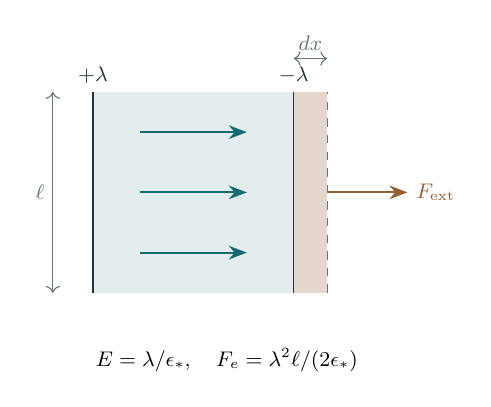
\begin{tikzpicture}[scale=.85,transform shape]

\fill[accent!12] (0,0) rectangle (3,3);
\draw[object] (0,0)--(0,3) node[above] {$+\lambda$};
\draw[object] (3,0)--(3,3) node[above] {$-\lambda$};
\fill[warm!25] (3,0) rectangle (3.5,3);
\draw[guide] (3.5,0)--(3.5,3);
\foreach \y in {.6,1.5,2.4}{\draw[motion] (.7,\y)--(2.3,\y);}
\draw[force] (3.5,1.5)--(4.7,1.5) node[right] {$F_{\rm ext}$};
\draw[axis,<->] (3,3.5)--(3.5,3.5) node[midway,above] {$dx$};
\draw[axis,<->] (-.6,0)--(-.6,3) node[midway,left] {$\ell$};
\node at (2,-1) {$E=\lambda/\epsilon_*,\quad F_e=\lambda^2\ell/(2\epsilon_*)$};

\end{tikzpicture}
\figcaption{解图综四.5B\quad 拉开带电线新增薄场区；受力只使用另一条线所生电场。}
\end{minipage}\end{center}
第（2）问，解图综四.5B先取无限长均匀带电直线，线密度$\lambda$。由平移和镜面对称性，场垂直直线，两侧大小相同；跨线取长$\ell$的矩形高斯线，通量只穿过两个长边：
\[
2E\ell=\frac{\lambda\ell}{\epsilon_*},\qquad
E_{\rm single}=\frac{\lambda}{2\epsilon_*}.
\]
再取长度$\ell$远大于间距$d$的两条平行线，电荷线密度分别为$\lambda,-\lambda$。忽略端部效应，间隙内两场同向相加，外侧抵消：
\[
E=\frac{\lambda}{\epsilon_*}.
\]
右侧带电线受到左侧所生的场$E_{\rm single}$，吸引力大小为
$F_e=\lambda\ell\,E_{\rm single}=\lambda^2\ell/(2\epsilon_*)$。
固定左线、用外力将右线缓慢拉开$dx$，外力做功
\[
dW=\frac{\lambda^2\ell}{2\epsilon_*}dx.
\]
新增加的匀强场面积是$\ell\,dx$，所以
\[
\boxed{w=\frac{dW}{\ell\,dx}
=\frac{\lambda^2}{2\epsilon_*}
=\frac12\epsilon_* E^2}.
\]
此特例验证了局域场能式及其系数。带电线所受的场由另一条线产生，其大小为间隙总场的一半，这给出了做功式中的二分之一。
图B的单条带电线可用给定点电荷场直接积分，说明两侧场强为何与到线的距离无关。将带电线取为$y$轴，在$(x,0)$处，$y'$位置电荷元为$\lambda\,dy'$，其横向分量为
\[
dE_x=\frac{\lambda}{2\pi\epsilon_*}\frac{x\,dy'}{x^2+y'^2}.
\]
纵向分量对$y'$为奇函数，成对抵消。对$x\ne0$，定限积分给
\[
E_x=\frac{\lambda x}{2\pi\epsilon_*}
\int_{-\infty}^{\infty}\frac{dy'}{x^2+y'^2}
=\frac{\lambda}{2\epsilon_*}\operatorname{sgn}x.
\]
由此，两侧各是大小相等、方向相反的匀强场。带电线处的受力场按两侧对称平均取值，单线自身的主值为零；加入另一条线后，右线所受的场恰为左线所生的$E_{\rm single}$。两线间的总场是两者相加后的$E=2E_{\rm single}$，所以做功式出现二分之一。

拉开过程保持两线上的电量及长度不变，原有间隙的场强也保持不变。外区两场抵消，原有内区的能量密度不变，新增能量只出现在宽$dx$、长$\ell$的细条中。缓慢移动使动能变化可以略去，外力功全部计入该细条场能。这同时交代了“做功除以新增面积”所需的电荷约束与准静态条件。无限长直线给出精确匀强场，有限线段的计算则取$\ell\gg d,dx$而忽略端部。

\begin{center}\begin{minipage}{.98\linewidth}\centering
\begin{tikzpicture}[scale=.85,transform shape]

\fill[accent!15,even odd rule] (0,0) circle (2) (0,0) circle (1.7);
\draw[object] (0,0) circle (2);
\draw[guide] (0,0) circle (1.7);
\fill (0,0) circle (2pt) node[below] {$O$};
\draw[guide] (0,0)--(2,0) node[midway,below] {$R$};
\draw[force] (2,0)--(1.3,0) node[above left] {收缩};
\node[align=left] at (5,1) {旧外区场不变\\薄环新建外场\\$dW=QE_Rd\ell$};
\node at (2,-3) {$E_R=(E_{\rm in}+E_{\rm out})/2$};

\end{tikzpicture}
\figcaption{解图综四.5C\quad 固定总电荷缓慢收缩圆环，新增场能确定作用于环上电荷的场。}
\end{minipage}\end{center}
第（3）问，解图综四.5C的圆环由旋转对称性和高斯定理给出
\[
E(r)=\begin{cases}
0,&r<R,\\
Q/(2\pi\epsilon_*r),&r>R.
\end{cases}
\]
圆环收缩时保持总电荷$Q$不变。让各电荷缓慢径向内移$d\ell>0$，旧外区$r>R$的场不变；内区仍无场，只有半径$R-d\ell$至$R$的薄环成为新增外场区。其面积约为$2\pi R\,d\ell$，所以
\[
dW=2\pi R\,d\ell\,
\frac12\epsilon_*\left(\frac{Q}{2\pi\epsilon_*R}\right)^2
=\frac{Q^2}{4\pi\epsilon_*R}d\ell.
\]
设环上排除自身元后的电场为径向外的$E_R$，外力克服它所做功为$QE_Rd\ell$。比较得到
\[
\boxed{E_R=\frac{Q}{4\pi\epsilon_*R}\quad\text{沿径向向外}}.
\]
它等于内外两侧极限场的平均$\frac12(E_{\rm in}+E_{\rm out})$，即外侧极限场的一半。环两侧存在场的跃变，故“环上电场”的取值方式需要说明；这里正是作用于环上电荷的对称主值。
圆环内外的场先由对称性确定方向，再由通量定出大小。取同心半径$r$的圆，切向分量由镜面对称性抵消，径向分量在圆周上恒定，所以$2\pi rE(r)=Q_{\rm in}(r)/\epsilon_*$。当$r<R$时包围电量为零；当$r>R$时包围电量为$Q$，得到图C所用的两侧场。

尽管带净电荷的整平面能量发散，这里的收缩功是有限的能量差。为写清这一点，在固定外半径$b>R$处截断，外场能为
\[
W(R;b)=\int_R^b\frac{Q^2}{4\pi\epsilon_*r}\,dr
=\frac{Q^2}{4\pi\epsilon_*}\ln\frac bR.
\]
收缩后两种配置在$r>R$处的场完全相同，能量差为
\[
W(R-d\ell;b)-W(R;b)
=\frac{Q^2}{4\pi\epsilon_*}\ln\frac{R}{R-d\ell}
=\frac{Q^2}{4\pi\epsilon_*R}d\ell+O(d\ell^2).
\]
外截断$b$在差值中消去，因而可用新增薄环的有限能量直接求环上受力场。正的收缩功说明电荷受到向外的排斥，外力向内克服它。两侧场的平均值表示除去自身电荷元后、其余电荷在该点施加的径向场；两侧跳变的差为$Q/(2\pi\epsilon_*R)$，对应环上线电荷密度$Q/(2\pi R)$除以$\epsilon_*$。

\begin{center}\begin{minipage}{.98\linewidth}\centering
\begin{tikzpicture}[scale=.85,transform shape]

\fill[accent!12] (0,0) circle (1.3);
\draw[object] (0,0) circle (1.3);
\draw[guide] (0,0) circle (2);
\draw[guide] (0,0)--(2,0) node[midway,below] {$r$};
\node at (0,.5) {$\sigma$};\node at (0,-.5) {$Q=\pi a^2\sigma$};
\node[align=left] at (5,.6) {$r<a:\ E=\sigma r/(2\epsilon_*)$\\$r>a:\ E=Q/(2\pi\epsilon_*r)$\\$W_{\rm out}\propto\ln(b/a)$};
\node at (2,-3) {圆盘内能有限，发散来自无穷远尾场};

\end{tikzpicture}
\figcaption{解图综四.5D\quad 圆对称例子明确显示dr/r的对数场能尾部。}
\end{minipage}\end{center}
第（4）问，先看解图综四.5D的均匀带电圆盘，半径$a$。圆内外的场分别为
\[
E(r)=\frac{\sigma r}{2\epsilon_*}\quad(r<a),\qquad
E(r)=\frac{\sigma a^2}{2\epsilon_*r}
=\frac{Q}{2\pi\epsilon_*r}\quad(r>a).
\]
外部$r=a$至截断半径$b$的能量为
\[
W_{\rm out}(b)=\int_a^b\frac12\epsilon_*E^2\,2\pi r\,dr
=\frac{Q^2}{4\pi\epsilon_*}\ln\frac ba
\ \longrightarrow\ \infty.
\]
慢衰减的$1/r$场在二维面积元$2\pi r\,dr$下留下$dr/r$的对数发散。
\begin{center}\begin{minipage}{.98\linewidth}\centering
\begin{tikzpicture}[scale=.76,transform shape]

\fill[accent!15] plot[smooth cycle] coordinates {(-.8,-.7)(-.4,.9)(.6,.6)(.8,-.2)(0,-.9)};
\draw[object] plot[smooth cycle] coordinates {(-.8,-.7)(-.4,.9)(.6,.6)(.8,-.2)(0,-.9)};
\draw[guide] (0,0) circle (1.3);\draw[object] (0,0) circle (2.2);
\draw[force] (2.2,0)--(3.1,0) node[right] {$\boldsymbol n$};
\node at (0,0) {$Q>0$};
\node[above] at (0,1.3) {$r_0$};\node[left] at (-2.2,0) {$C_r$};
\node[align=left] at (6,.5) {$\oint E_n\,d\ell=Q/\epsilon_*$\\$\oint E^2d\ell\ge Q^2/(2\pi\epsilon_*^2r)$};
\node at (2.8,-3) {外区不必圆对称；每个包围圆的通量给能量下界};

\end{tikzpicture}
\figcaption{解图综四.5E\quad 任意有界电荷区外取同心圆，用柯西不等式代替场的逐点比较。}
\end{minipage}\end{center}
为把结论扩展到不规则区域，解图综四.5E取一个半径$r_0$的圆包住全部电荷，总电量$Q=\sigma S>0$。对任意$r>r_0$，高斯定理给
$\oint_{C_r}\boldsymbol E\cdot\boldsymbol n\,d\ell=Q/\epsilon_*$。
用柯西不等式，
\[
\left(\oint_{C_r}\boldsymbol E\cdot\boldsymbol n\,d\ell\right)^2
\le(2\pi r)\oint_{C_r}(\boldsymbol E\cdot\boldsymbol n)^2d\ell
\le(2\pi r)\oint_{C_r}|\boldsymbol E|^2d\ell.
\]
因此薄圆环中的场能满足
\[
dW=\frac12\epsilon_*\left(\oint_{C_r}|\boldsymbol E|^2d\ell\right)dr
\ge\frac{Q^2}{4\pi\epsilon_*}\frac{dr}{r}.
\]
从$r_0$积分到$b$便得
\[
\boxed{W(b)\ge
\frac{Q^2}{4\pi\epsilon_*}\ln\frac b{r_0}\longrightarrow\infty}.
\]
外区场可以不沿径向，子区域场能之间也可以有交叉项；包围圆的通量仍给出上述下界。总通量已给出足够的正下界，故任意题设区域都有无限的全平面场能。

图D的圆盘还可把内外两区的能量分开。圆内半径$r$所包围电量为$\sigma\pi r^2$，因此圆内场从中心的零线性增至表面值。将这个场代入面积积分，
\[
W_{\rm in}=\int_0^a\frac12\epsilon_*
\left(\frac{\sigma r}{2\epsilon_*}\right)^2\,2\pi r\,dr
=\frac{\pi\sigma^2a^4}{16\epsilon_*}
=\frac{Q^2}{16\pi\epsilon_*}.
\]
于是截断圆盘总能量为$W(b)=Q^2/(16\pi\epsilon_*)+[Q^2/(4\pi\epsilon_*)]\ln(b/a)$。内区有限，发散项全部积累在越来越远的圆环中；把截断半径加倍，每次增加的外场能都为$Q^2\ln2/(4\pi\epsilon_*)$，所以无限多次加倍产生无界总能量。

对于图E中的均匀不规则区域，半径$r_0$的包围圆只用于隔开电荷区与远区。它与电荷分布本身的形状无关；在每一个更大圆周上，径向场可以随方位改变，场也可有切向分量。柯西不等式的第一步把固定总通量与径向分量的平方联系起来，第二步利用$E_r^2\le|\boldsymbol E|^2$。只有在该圆周上场处处径向且大小恒定时，两步等号同时成立。圆盘与圆环的圆对称外场恰好达到下限，所以该系数已经由明确可算的配置给出。

若保留“取出一个圆形子区域”的分解思路，设两部分电荷场分别为$\boldsymbol E_1,\boldsymbol E_2$，在同一个截断区域内精确地有
\[
W(b)=W_1(b)+W_2(b)+
\epsilon_*\int_{r<b}\boldsymbol E_1\cdot\boldsymbol E_2\,dS.
\]
前两项非负，第三项取决于两矢量的相对方向，宜与另外两项一起处理。对子区域各自的圆对称外场，圆形部分的对数积分仍然成立；而全分布发散的结论由图E的总通量下界直接得出，涵盖全部交叉项。

也可从远处看出这一结论的物理原因。将有界电荷区置于半径$a_0$内，观察点写成$\boldsymbol x=r\boldsymbol n$，当$r\gg a_0$时，单个电荷元的场核满足
\[
\frac{r\boldsymbol n-\boldsymbol y}{|r\boldsymbol n-\boldsymbol y|^2}
=\frac{\boldsymbol n}{r}
+\frac{2\boldsymbol n(\boldsymbol n\cdot\boldsymbol y)-\boldsymbol y}{r^2}
+O(r^{-3}).
\]
积分后，首项只含总电量$Q$：
$\boldsymbol E=Q\boldsymbol n/(2\pi\epsilon_*r)+O(r^{-2})$。
它的平方乘圆环面积元$2\pi r\,dr$产生对数项；含电荷形状和偏心位置的下一阶修正，在远区积分中有限。这个远场图像说明，高斯下界由总电量决定：非零净电荷产生$1/r$项，改变区域形状只影响下一阶项。

最后把远处发散与带电区附近的有限能量分开说明。题设区域面积$S>0$、密度$\sigma>0$，所以$Q=\sigma S>0$，通量下限的系数严格为正。面电荷的场核大小与$1/s$成正比，这个局部奇性在二维面积积分中可积。若全部电荷位于半径$r_0$内，观察点也在该圆内，则两点间距至多为$2r_0$，由三角不等式有
\[
|\boldsymbol E(\boldsymbol x)|
\le\frac{\sigma}{2\pi\epsilon_*}
\int_S\frac{d^2y}{|\boldsymbol x-\boldsymbol y|}
\le\frac{\sigma}{2\pi\epsilon_*}
\int_0^{2r_0}\frac{2\pi s\,ds}{s}
=\frac{2\sigma r_0}{\epsilon_*}.
\]
因此包围圆内的场能不超过$2\pi\sigma^2r_0^4/\epsilon_*$，是有限量。即使区域轮廓不规则，这个估计仍适用，因为积分区域包含在以观察点为中心、半径$2r_0$的圆内。全平面能量的无界增长由远处的无限多层圆环产生，与面电荷单元附近的局部积分有清楚的区别。


\Needspace{13\baselineskip}

\pdfbookmark[2]{第 6 题 相对论库仑轨道的近日点进动}{q6}

\section*{第 6 题\quad 相对论库仑轨道的近日点进动}\label{q:6}


惯性系中固定点电荷$Q>0$位于平面内的$O$，另一静质量为$m_0$、带电量$-q$（$q>0$）的粒子$P$受其库仑力，沿有界、非圆轨道运动。其初始总相对论能量为$E_0$，包括静能和电势能；关于$O$的初始角动量为$L_0>0$。令
\[
\kappa=\frac{qQ}{4\pi\epsilon_0},\qquad
\eta=\frac{\kappa}{L_0c}\ll1.
\]
这里使用三维真空库仑定律，但粒子运动限于一个平面；忽略辐射反作用。

（1）证明忽略$\eta^2$的零级近似轨道为椭圆。（2）求保留相对论动力学后的轨道方程，说明相邻两次近日点之间的转角，进而给出每个径向周期的进动角及其最低阶近似。


\begin{center}\begin{minipage}{.98\linewidth}\centering
\begin{tikzpicture}[scale=.85,transform shape]

\draw[traj,domain=0:400,samples=200] plot ({2*cos(\x)/(1+.45*cos(.96*\x))},{2*sin(\x)/(1+.45*cos(.96*\x))});
\fill (0,0) circle (2pt) node[below] {$O,+Q$};
\node at (0,-3.6) {有界非圆轨道，图中进动为示意};
\draw[guide] (0,0)--(1.38,0) node[midway,below] {$r$};

\end{tikzpicture}
\figcaption{图综四.6\quad 三维库仑力限于平面运动，相对论动力学使近日点方向改变。}
\end{minipage}\end{center}

\Needspace{6\baselineskip}\subsection*{解答}


图综四.6中的力始终沿$PO$，动量为$\boldsymbol p=\gamma m_0\boldsymbol v$，动力学采用$\boldsymbol F=d\boldsymbol p/dt$。记$\mathfrak m=\gamma m_0$为便于推导的瞬时惯性因子，静质量$m_0$并未改变。
\begin{center}\begin{minipage}{.98\linewidth}\centering
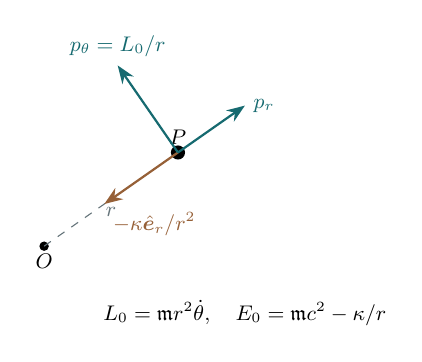
\begin{tikzpicture}[scale=.85,transform shape]

\fill (0,0) circle (2pt) node[below] {$O$};
\fill (2,1.4) circle (3pt) node[above] {$P$};
\draw[guide] (0,0)--(2,1.4) node[midway,below] {$r$};
\draw[force] (2,1.4)--(.9,.63) node[below right] {$-\kappa\hat{\boldsymbol e}_r/r^2$};
\draw[motion] (2,1.4)--(1.1,2.7) node[above] {$p_\theta=L_0/r$};
\draw[motion] (2,1.4)--(3,2.1) node[right] {$p_r$};
\node at (3,-1) {$L_0=\mathfrak m r^2\dot\theta,\quad E_0=\mathfrak m c^2-\kappa/r$};

\end{tikzpicture}
\figcaption{解图综四.6A\quad 极坐标动量的径向、切向分量；守恒的是总能量与角动量。}
\end{minipage}\end{center}
解图综四.6A在极坐标基矢中分解动量。动力学方程为
\[
\frac{d(\mathfrak m\boldsymbol v)}{dt}
=-\frac{\kappa}{r^2}\hat{\boldsymbol e}_r.
\]
动量的分量式包含极坐标基矢的转动。具体地，
\[
\boldsymbol p=p_r\hat{\boldsymbol e}_r+p_\theta\hat{\boldsymbol e}_\theta,
\quad
\dot{\hat{\boldsymbol e}}_r=\dot\theta\hat{\boldsymbol e}_\theta,\quad
\dot{\hat{\boldsymbol e}}_\theta=-\dot\theta\hat{\boldsymbol e}_r.
\]
由此$d\boldsymbol p/dt$的径向分量为$\dot p_r-p_\theta\dot\theta$，角向分量为$\dot p_\theta+p_r\dot\theta$。代入$p_r=\mathfrak m\dot r$、$p_\theta=\mathfrak m r\dot\theta$，恰好得到图A后的两个分量方程。径向式中的$-\mathfrak mr\dot\theta^2$由基矢转动产生；将$\mathfrak m$保留在时间导数内，才能同时包含动量大小随电势改变的影响。

径向和角向分量分别为
\[
\frac d{dt}(\mathfrak m\dot r)-\mathfrak m r\dot\theta^2
=-\frac{\kappa}{r^2},\qquad
\dot{\mathfrak m}r\dot\theta
+\mathfrak m(2\dot r\dot\theta+r\ddot\theta)=0.
\]
角向式乘以$r$正好是
\[
\frac d{dt}(\mathfrak m r^2\dot\theta)=0,
\qquad
\boxed{L=\mathfrak m r^2\dot\theta=L_0}.
\]
静电力保守，总能量也守恒：
\[
\boxed{E_0=\mathfrak m c^2-\frac{\kappa}{r}},\qquad
\mathfrak m=\frac{E_0+\kappa/r}{c^2}.
\]
守恒的$E_0$包括电势能；粒子靠近中心时，$\mathfrak m c^2$随$r$减小而增大。

为消去时间，令$u=1/r$，用撇号表示对$\theta$求导。由角动量式，
\[
\dot\theta=\frac{L_0u^2}{\mathfrak m},\qquad
\mathfrak m\dot r
=\mathfrak m\frac{dr}{d\theta}\dot\theta=-L_0u'.
\]
用角动量把时间换成极角时，有$\frac d{dt}=\dot\theta\frac d{d\theta}$。因此
\[
\frac d{dt}(\mathfrak m\dot r)
=-L_0\frac{du'}{d\theta}\dot\theta
=-\frac{L_0^2u^2}{\mathfrak m}u'',
\qquad
\mathfrak m r\dot\theta^2=\frac{L_0^2u^3}{\mathfrak m}.
\]
这两项的共同因子为$L_0^2u^2/\mathfrak m$，约去以后右边成为$\kappa\mathfrak m/L_0^2$。总能量给出的$\mathfrak m=E_0/c^2+\kappa u/c^2$在此产生常量项$b$和与$u$成正比的$\eta^2u$；正是后一项把径向相位系数从1降为$\nu$。这里保留有限的库仑场和有限的轨道尺度，只在零级方程中略去无量纲小修正$\eta^2$。

径向方程变为
\[
-\frac{L_0^2u^2}{\mathfrak m}u''
-\frac{L_0^2u^3}{\mathfrak m}
=-\kappa u^2.
\]
除以$-L_0^2u^2/\mathfrak m$，再用能量式，得到
\[
u''+u=\frac{\kappa\mathfrak m}{L_0^2}
=\frac{\kappa E_0}{L_0^2c^2}
+\frac{\kappa^2}{L_0^2c^2}u.
\]
记$b=\kappa E_0/(L_0^2c^2)$，于是精确轨道方程为
\[
\boxed{u''+(1-\eta^2)u=b}.
\]
\begin{center}\begin{minipage}{.98\linewidth}\centering
\begin{tikzpicture}[scale=.85,transform shape]

\draw[object,domain=0:360,samples=160] plot ({2*cos(\x)/(1+.5*cos(\x))},{2*sin(\x)/(1+.5*cos(\x))});
\draw[axis] (-4.5,0)--(2.2,0) node[right] {近拱线};
\fill (0,0) circle (2pt) node[below] {$O$};
\fill (1.3333,0) circle (2pt) node[above] {近日点};
\fill (-4,0) circle (2pt) node[above] {远日点};
\node at (-1,-3.2) {$\eta^2\to0:\ r=p/[1+e\cos(\theta-\theta_p)]$};

\end{tikzpicture}
\figcaption{解图综四.6B\quad 零级椭圆的两个径向转折点；焦点$O$与椭圆中心位于近拱线的不同位置。}
\end{minipage}\end{center}
第（1）问，忽略$\eta^2$后，解图综四.6B对应
\[
u''+u=b,\qquad
u=b+A\cos(\theta-\theta_p)
=b[1+e\cos(\theta-\theta_p)].
\]
图B中零级方程的通解也可先写成$u=b+C\cos\theta+D\sin\theta$。将$C,D$合并为振幅和相位，$A=\sqrt{C^2+D^2}$、$C=A\cos\theta_p$、$D=A\sin\theta_p$，便得到$u=b+A\cos(\theta-\theta_p)$。以近日点方向作极轴时$\theta_p=0$，$e=A/b$。这说明偏心率与近日点方向来自两个初始条件，而半通径由守恒量确定；椭圆中心与力心$O$的区别落实在图B所标的焦点位置上。

以$p=1/b=L_0^2c^2/(\kappa E_0)$记半通径，
\[
\boxed{r=\frac{p}{1+e\cos(\theta-\theta_p)}}.
\]
有界且不碰中心的轨道要求$0\le e<1$；题设非圆使$e>0$。所以这是以$O$为一个焦点的椭圆，$\theta_p$给近日点方向。零级方程保留库仑作用与有限轨道尺度，略去无量纲相对论校正项$\eta^2u$。

第（2）问，令$\nu=\sqrt{1-\eta^2}$。因为$\eta\ll1$，$\nu$为正实数，完整解可写为
\[
u=\frac b{\nu^2}
\left[1+e'\cos\bigl(\nu(\theta-\theta_p)\bigr)\right].
\]
因此
\[
\boxed{r=\frac{p'}{1+e'\cos[\nu(\theta-\theta_p)]}},
\quad
\boxed{p'=\frac{\nu^2}{b}
=\frac{L_0^2c^2-\kappa^2}{\kappa E_0}}.
\]
$e'$由初始径向运动确定，有界非圆轨道取$0<e'<1$。径向形状随$\nu\theta$重复，但极角本身不再每$2\pi$恰好回到同一近日点。
\begin{center}\begin{minipage}{.98\linewidth}\centering
\begin{tikzpicture}[scale=.85,transform shape]

\draw[traj,domain=0:423.5294,samples=250] plot ({1.5*cos(\x)/(1+.45*cos(.85*\x))},{1.5*sin(\x)/(1+.45*cos(.85*\x))});
\draw[guide] (0,0)--(1.6,0);
\draw[guide] (0,0)--({1.6*cos(63.5294)},{1.6*sin(63.5294)});
\draw[guide] (.6,0) arc[start angle=0,end angle=63.5294,radius=.6];
\node[right] at (.75,.45) {$\Delta\varpi$};
\fill (0,0) circle (2pt) node[below] {$O$};
\fill (1.03448,0) circle (2pt) node[below] {$P_0$};
\fill ({1.03448*cos(63.5294)},{1.03448*sin(63.5294)}) circle (2pt) node[above right] {$P_1$};
\node[align=left] at (4.7,-.2) {$\nu\Theta_r=2\pi$\\$\Delta\varpi=\Theta_r-2\pi>0$\\示意图放大了进动};

\end{tikzpicture}
\figcaption{解图综四.6C\quad 相邻近日点的径向相位差为$2\pi$，实际极角比整周多出正进动角。}
\end{minipage}\end{center}
\textbf{图中相位与轨道常量。} 令$\chi=\nu(\theta-\theta_p)$，解图综四.6D把倒数半径归一化到平均值$u_c=b/\nu^2$，画出$u/u_c=1+e'\cos\chi$与同振幅的零级振荡。为了在图上看清相位差，曲线采用$\eta=0.3$的精确模型作示意；小参数展开仍按$\eta\ll1$使用。两条曲线起初同时在近日点，随后精确径向相位逐渐落后于空间极角，第二个近日点出现在$\theta>2\pi$的位置，近日点方向因而沿绕行方向前移。
\begin{center}\begin{minipage}{.98\linewidth}\centering
\begin{tikzpicture}[scale=0.72,transform shape]
\draw[axis] (0,0)--(6.2,0);\draw[axis] (0,0)--(0,3.4000000000000004);
\draw[thin,color=muted] (0.0000000,0)--(0.0000000,-.07);\node[below] at (0.0000000,-.09) {$0$};
\draw[thin,color=muted] (2.7272727,0)--(2.7272727,-.07);\node[below] at (2.7272727,-.09) {$1$};
\draw[thin,color=muted] (5.4545455,0)--(5.4545455,-.07);\node[below] at (5.4545455,-.09) {$2$};
\draw[thin,color=muted] (0,0.3200000)--(-.07,0.3200000);\node[left] at (-.09,0.3200000) {$.6$};
\draw[thin,color=muted] (0,1.6000000)--(-.07,1.6000000);\node[left] at (-.09,1.6000000) {$1$};
\draw[thin,color=muted] (0,2.8800000)--(-.07,2.8800000);\node[left] at (-.09,2.8800000) {$1.4$};
\node[below] at (3.0,-.64) {极角$\theta/(2\pi)$};\node[above right] at (0,3.45) {$u/u_c$};
\draw[traj] plot coordinates {(0.0000000,2.8800000) (0.0090909,2.8797445) (0.0181818,2.8789783) (0.0272727,2.8777015) (0.0363636,2.8759147) (0.0454545,2.8736186) (0.0545455,2.8708141) (0.0636364,2.8675024) (0.0727273,2.8636847) (0.0818182,2.8593627) (0.0909091,2.8545379) (0.1000000,2.8492124) (0.1090909,2.8433883) (0.1181818,2.8370679) (0.1272727,2.8302536) (0.1363636,2.8229483) (0.1454545,2.8151549) (0.1545455,2.8068764) (0.1636364,2.7981162) (0.1727273,2.7888778) (0.1818182,2.7791648) (0.1909091,2.7689811) (0.2000000,2.7583308) (0.2090909,2.7472182) (0.2181818,2.7356476) (0.2272727,2.7236238) (0.2363636,2.7111514) (0.2454545,2.6982355) (0.2545455,2.6848813) (0.2636364,2.6710940) (0.2727273,2.6568792) (0.2818182,2.6422425) (0.2909091,2.6271898) (0.3000000,2.6117271) (0.3090909,2.5958605) (0.3181818,2.5795964) (0.3272727,2.5629414) (0.3363636,2.5459019) (0.3454545,2.5284849) (0.3545455,2.5106973) (0.3636364,2.4925462) (0.3727273,2.4740388) (0.3818182,2.4551825) (0.3909091,2.4359849) (0.4000000,2.4164536) (0.4090909,2.3965964) (0.4181818,2.3764212) (0.4272727,2.3559361) (0.4363636,2.3351493) (0.4454545,2.3140690) (0.4545455,2.2927037) (0.4636364,2.2710619) (0.4727273,2.2491523) (0.4818182,2.2269835) (0.4909091,2.2045645) (0.5000000,2.1819042) (0.5090909,2.1590115) (0.5181818,2.1358958) (0.5272727,2.1125661) (0.5363636,2.0890319) (0.5454545,2.0653024) (0.5545455,2.0413873) (0.5636364,2.0172959) (0.5727273,1.9930380) (0.5818182,1.9686232) (0.5909091,1.9440612) (0.6000000,1.9193619) (0.6090909,1.8945352) (0.6181818,1.8695908) (0.6272727,1.8445389) (0.6363636,1.8193893) (0.6454545,1.7941522) (0.6545455,1.7688376) (0.6636364,1.7434556) (0.6727273,1.7180163) (0.6818182,1.6925300) (0.6909091,1.6670066) (0.7000000,1.6414566) (0.7090909,1.6158900) (0.7181818,1.5903170) (0.7272727,1.5647480) (0.7363636,1.5391929) (0.7454545,1.5136622) (0.7545455,1.4881659) (0.7636364,1.4627143) (0.7727273,1.4373174) (0.7818182,1.4119855) (0.7909091,1.3867287) (0.8000000,1.3615570) (0.8090909,1.3364804) (0.8181818,1.3115090) (0.8272727,1.2866528) (0.8363636,1.2619217) (0.8454545,1.2373255) (0.8545455,1.2128741) (0.8636364,1.1885772) (0.8727273,1.1644445) (0.8818182,1.1404857) (0.8909091,1.1167103) (0.9000000,1.0931278) (0.9090909,1.0697476) (0.9181818,1.0465791) (0.9272727,1.0236315) (0.9363636,1.0009139) (0.9454545,0.9784355) (0.9545455,0.9562051) (0.9636364,0.9342318) (0.9727273,0.9125242) (0.9818182,0.8910910) (0.9909091,0.8699408) (1.0000000,0.8490820) (1.0090909,0.8285229) (1.0181818,0.8082717) (1.0272727,0.7883366) (1.0363636,0.7687255) (1.0454545,0.7494462) (1.0545455,0.7305063) (1.0636364,0.7119136) (1.0727273,0.6936753) (1.0818182,0.6757988) (1.0909091,0.6582912) (1.1000000,0.6411595) (1.1090909,0.6244105) (1.1181818,0.6080509) (1.1272727,0.5920873) (1.1363636,0.5765260) (1.1454545,0.5613732) (1.1545455,0.5466350) (1.1636364,0.5323172) (1.1727273,0.5184257) (1.1818182,0.5049658) (1.1909091,0.4919430) (1.2000000,0.4793626) (1.2090909,0.4672294) (1.2181818,0.4555484) (1.2272727,0.4443242) (1.2363636,0.4335613) (1.2454545,0.4232640) (1.2545455,0.4134364) (1.2636364,0.4040824) (1.2727273,0.3952058) (1.2818182,0.3868100) (1.2909091,0.3788986) (1.3000000,0.3714745) (1.3090909,0.3645408) (1.3181818,0.3581003) (1.3272727,0.3521555) (1.3363636,0.3467087) (1.3454545,0.3417623) (1.3545455,0.3373180) (1.3636364,0.3333778) (1.3727273,0.3299432) (1.3818182,0.3270155) (1.3909091,0.3245959) (1.4000000,0.3226854) (1.4090909,0.3212847) (1.4181818,0.3203945) (1.4272727,0.3200151) (1.4363636,0.3201465) (1.4454545,0.3207888) (1.4545455,0.3219417) (1.4636364,0.3236048) (1.4727273,0.3257773) (1.4818182,0.3284585) (1.4909091,0.3316472) (1.5000000,0.3353422) (1.5090909,0.3395420) (1.5181818,0.3442449) (1.5272727,0.3494490) (1.5363636,0.3551523) (1.5454545,0.3613525) (1.5545455,0.3680471) (1.5636364,0.3752335) (1.5727273,0.3829087) (1.5818182,0.3910698) (1.5909091,0.3997134) (1.6000000,0.4088361) (1.6090909,0.4184342) (1.6181818,0.4285040) (1.6272727,0.4390414) (1.6363636,0.4500422) (1.6454545,0.4615021) (1.6545455,0.4734163) (1.6636364,0.4857803) (1.6727273,0.4985890) (1.6818182,0.5118373) (1.6909091,0.5255200) (1.7000000,0.5396315) (1.7090909,0.5541664) (1.7181818,0.5691186) (1.7272727,0.5844824) (1.7363636,0.6002515) (1.7454545,0.6164197) (1.7545455,0.6329804) (1.7636364,0.6499272) (1.7727273,0.6672532) (1.7818182,0.6849515) (1.7909091,0.7030151) (1.8000000,0.7214366) (1.8090909,0.7402089) (1.8181818,0.7593244) (1.8272727,0.7787754) (1.8363636,0.7985542) (1.8454545,0.8186530) (1.8545455,0.8390636) (1.8636364,0.8597779) (1.8727273,0.8807877) (1.8818182,0.9020846) (1.8909091,0.9236601) (1.9000000,0.9455055) (1.9090909,0.9676122) (1.9181818,0.9899713) (1.9272727,1.0125739) (1.9363636,1.0354110) (1.9454545,1.0584734) (1.9545455,1.0817520) (1.9636364,1.1052374) (1.9727273,1.1289204) (1.9818182,1.1527914) (1.9909091,1.1768408) (2.0000000,1.2010592) (2.0090909,1.2254369) (2.0181818,1.2499640) (2.0272727,1.2746308) (2.0363636,1.2994276) (2.0454545,1.3243443) (2.0545455,1.3493710) (2.0636364,1.3744978) (2.0727273,1.3997146) (2.0818182,1.4250113) (2.0909091,1.4503779) (2.1000000,1.4758042) (2.1090909,1.5012801) (2.1181818,1.5267954) (2.1272727,1.5523399) (2.1363636,1.5779034) (2.1454545,1.6034757) (2.1545455,1.6290467) (2.1636364,1.6546060) (2.1727273,1.6801436) (2.1818182,1.7056492) (2.1909091,1.7311126) (2.2000000,1.7565237) (2.2090909,1.7818723) (2.2181818,1.8071483) (2.2272727,1.8323416) (2.2363636,1.8574422) (2.2454545,1.8824400) (2.2545455,1.9073250) (2.2636364,1.9320875) (2.2727273,1.9567173) (2.2818182,1.9812048) (2.2909091,2.0055401) (2.3000000,2.0297135) (2.3090909,2.0537154) (2.3181818,2.0775362) (2.3272727,2.1011664) (2.3363636,2.1245965) (2.3454545,2.1478173) (2.3545455,2.1708194) (2.3636364,2.1935936) (2.3727273,2.2161309) (2.3818182,2.2384223) (2.3909091,2.2604588) (2.4000000,2.2822317) (2.4090909,2.3037323) (2.4181818,2.3249520) (2.4272727,2.3458823) (2.4363636,2.3665149) (2.4454545,2.3868415) (2.4545455,2.4068541) (2.4636364,2.4265446) (2.4727273,2.4459052) (2.4818182,2.4649281) (2.4909091,2.4836058) (2.5000000,2.5019308) (2.5090909,2.5198958) (2.5181818,2.5374936) (2.5272727,2.5547171) (2.5363636,2.5715596) (2.5454545,2.5880143) (2.5545455,2.6040747) (2.5636364,2.6197342) (2.5727273,2.6349867) (2.5818182,2.6498261) (2.5909091,2.6642464) (2.6000000,2.6782420) (2.6090909,2.6918071) (2.6181818,2.7049365) (2.6272727,2.7176248) (2.6363636,2.7298670) (2.6454545,2.7416582) (2.6545455,2.7529937) (2.6636364,2.7638689) (2.6727273,2.7742796) (2.6818182,2.7842216) (2.6909091,2.7936909) (2.7000000,2.8026837) (2.7090909,2.8111965) (2.7181818,2.8192258) (2.7272727,2.8267684) (2.7363636,2.8338214) (2.7454545,2.8403819) (2.7545455,2.8464472) (2.7636364,2.8520151) (2.7727273,2.8570832) (2.7818182,2.8616495) (2.7909091,2.8657122) (2.8000000,2.8692697) (2.8090909,2.8723206) (2.8181818,2.8748636) (2.8272727,2.8768977) (2.8363636,2.8784222) (2.8454545,2.8794363) (2.8545455,2.8799398) (2.8636364,2.8799324) (2.8727273,2.8794140) (2.8818182,2.8783850) (2.8909091,2.8768457) (2.9000000,2.8747968) (2.9090909,2.8722390) (2.9181818,2.8691733) (2.9272727,2.8656011) (2.9363636,2.8615237) (2.9454545,2.8569428) (2.9545455,2.8518601) (2.9636364,2.8462778) (2.9727273,2.8401980) (2.9818182,2.8336231) (2.9909091,2.8265559) (3.0000000,2.8189990) (3.0090909,2.8109556) (3.0181818,2.8024288) (3.0272727,2.7934221) (3.0363636,2.7839390) (3.0454545,2.7739833) (3.0545455,2.7635590) (3.0636364,2.7526703) (3.0727273,2.7413215) (3.0818182,2.7295171) (3.0909091,2.7172618) (3.1000000,2.7045606) (3.1090909,2.6914185) (3.1181818,2.6778408) (3.1272727,2.6638328) (3.1363636,2.6494002) (3.1454545,2.6345487) (3.1545455,2.6192843) (3.1636364,2.6036130) (3.1727273,2.5875411) (3.1818182,2.5710750) (3.1909091,2.5542213) (3.2000000,2.5369867) (3.2090909,2.5193782) (3.2181818,2.5014026) (3.2272727,2.4830673) (3.2363636,2.4643794) (3.2454545,2.4453466) (3.2545455,2.4259763) (3.2636364,2.4062763) (3.2727273,2.3862545) (3.2818182,2.3659188) (3.2909091,2.3452774) (3.3000000,2.3243386) (3.3090909,2.3031106) (3.3181818,2.2816020) (3.3272727,2.2598213) (3.3363636,2.2377772) (3.3454545,2.2154785) (3.3545455,2.1929342) (3.3636364,2.1701532) (3.3727273,2.1471446) (3.3818182,2.1239177) (3.3909091,2.1004816) (3.4000000,2.0768457) (3.4090909,2.0530195) (3.4181818,2.0290125) (3.4272727,2.0048342) (3.4363636,1.9804943) (3.4454545,1.9560026) (3.4545455,1.9313687) (3.4636364,1.9066026) (3.4727273,1.8817141) (3.4818182,1.8567132) (3.4909091,1.8316098) (3.5000000,1.8064139) (3.5090909,1.7811357) (3.5181818,1.7557851) (3.5272727,1.7303724) (3.5363636,1.7049076) (3.5454545,1.6794009) (3.5545455,1.6538626) (3.5636364,1.6283027) (3.5727273,1.6027316) (3.5818182,1.5771594) (3.5909091,1.5515962) (3.6000000,1.5260524) (3.6090909,1.5005382) (3.6181818,1.4750636) (3.6272727,1.4496389) (3.6363636,1.4242742) (3.6454545,1.3989796) (3.6545455,1.3737653) (3.6636364,1.3486413) (3.6727273,1.3236177) (3.6818182,1.2987043) (3.6909091,1.2739112) (3.7000000,1.2492483) (3.7090909,1.2247254) (3.7181818,1.2003522) (3.7272727,1.1761386) (3.7363636,1.1520942) (3.7454545,1.1282286) (3.7545455,1.1045512) (3.7636364,1.0810717) (3.7727273,1.0577992) (3.7818182,1.0347432) (3.7909091,1.0119129) (3.8000000,0.9893172) (3.8090909,0.9669653) (3.8181818,0.9448661) (3.8272727,0.9230284) (3.8363636,0.9014610) (3.8454545,0.8801723) (3.8545455,0.8591710) (3.8636364,0.8384653) (3.8727273,0.8180637) (3.8818182,0.7979742) (3.8909091,0.7782048) (3.9000000,0.7587634) (3.9090909,0.7396578) (3.9181818,0.7208956) (3.9272727,0.7024843) (3.9363636,0.6844313) (3.9454545,0.6667438) (3.9545455,0.6494287) (3.9636364,0.6324931) (3.9727273,0.6159436) (3.9818182,0.5997870) (3.9909091,0.5840296) (4.0000000,0.5686777) (4.0090909,0.5537375) (4.0181818,0.5392149) (4.0272727,0.5251158) (4.0363636,0.5114456) (4.0454545,0.4982100) (4.0545455,0.4854142) (4.0636364,0.4730633) (4.0727273,0.4611622) (4.0818182,0.4497156) (4.0909091,0.4387282) (4.1000000,0.4282044) (4.1090909,0.4181483) (4.1181818,0.4085639) (4.1272727,0.3994551) (4.1363636,0.3908255) (4.1454545,0.3826785) (4.1545455,0.3750175) (4.1636364,0.3678454) (4.1727273,0.3611651) (4.1818182,0.3549793) (4.1909091,0.3492905) (4.2000000,0.3441009) (4.2090909,0.3394126) (4.2181818,0.3352275) (4.2272727,0.3315473) (4.2363636,0.3283733) (4.2454545,0.3257069) (4.2545455,0.3235492) (4.2636364,0.3219010) (4.2727273,0.3207629) (4.2818182,0.3201355) (4.2909091,0.3200189) (4.3000000,0.3204132) (4.3090909,0.3213183) (4.3181818,0.3227338) (4.3272727,0.3246591) (4.3363636,0.3270935) (4.3454545,0.3300359) (4.3545455,0.3334853) (4.3636364,0.3374402) (4.3727273,0.3418991) (4.3818182,0.3468602) (4.3909091,0.3523214) (4.4000000,0.3582807) (4.4090909,0.3647356) (4.4181818,0.3716836) (4.4272727,0.3791219) (4.4363636,0.3870475) (4.4454545,0.3954573) (4.4545455,0.4043478) (4.4636364,0.4137156) (4.4727273,0.4235570) (4.4818182,0.4338679) (4.4909091,0.4446443) (4.5000000,0.4558818) (4.5090909,0.4675761) (4.5181818,0.4797223) (4.5272727,0.4923157) (4.5363636,0.5053513) (4.5454545,0.5188238) (4.5545455,0.5327279) (4.5636364,0.5470579) (4.5727273,0.5618083) (4.5818182,0.5769730) (4.5909091,0.5925461) (4.6000000,0.6085214) (4.6090909,0.6248924) (4.6181818,0.6416526) (4.6272727,0.6587953) (4.6363636,0.6763138) (4.6454545,0.6942009) (4.6545455,0.7124496) (4.6636364,0.7310526) (4.6727273,0.7500024) (4.6818182,0.7692915) (4.6909091,0.7889121) (4.7000000,0.8088566) (4.7090909,0.8291168) (4.7181818,0.8496847) (4.7272727,0.8705521) (4.7363636,0.8917107) (4.7454545,0.9131520) (4.7545455,0.9348675) (4.7636364,0.9568484) (4.7727273,0.9790861) (4.7818182,1.0015716) (4.7909091,1.0242960) (4.8000000,1.0472502) (4.8090909,1.0704250) (4.8181818,1.0938112) (4.8272727,1.1173994) (4.8363636,1.1411803) (4.8454545,1.1651443) (4.8545455,1.1892819) (4.8636364,1.2135834) (4.8727273,1.2380392) (4.8818182,1.2626395) (4.8909091,1.2873744) (4.9000000,1.3122341) (4.9090909,1.3372087) (4.9181818,1.3622881) (4.9272727,1.3874625) (4.9363636,1.4127216) (4.9454545,1.4380556) (4.9545455,1.4634542) (4.9636364,1.4889072) (4.9727273,1.5144047) (4.9818182,1.5399362) (4.9909091,1.5654918) (5.0000000,1.5910611) (5.0090909,1.6166341) (5.0181818,1.6422003) (5.0272727,1.6677497) (5.0363636,1.6932721) (5.0454545,1.7187573) (5.0545455,1.7441950) (5.0636364,1.7695752) (5.0727273,1.7948877) (5.0818182,1.8201224) (5.0909091,1.8452693) (5.1000000,1.8703182) (5.1090909,1.8952593) (5.1181818,1.9200825) (5.1272727,1.9447779) (5.1363636,1.9693357) (5.1454545,1.9937461) (5.1545455,2.0179993) (5.1636364,2.0420857) (5.1727273,2.0659956) (5.1818182,2.0897195) (5.1909091,2.1132479) (5.2000000,2.1365715) (5.2090909,2.1596809) (5.2181818,2.1825669) (5.2272727,2.2052203) (5.2363636,2.2276322) (5.2454545,2.2497935) (5.2545455,2.2716955) (5.2636364,2.2933294) (5.2727273,2.3146865) (5.2818182,2.3357583) (5.2909091,2.3565365) (5.3000000,2.3770127) (5.3090909,2.3971787) (5.3181818,2.4170265) (5.3272727,2.4365483) (5.3363636,2.4557361) (5.3454545,2.4745823) (5.3545455,2.4930794) (5.3636364,2.5112201) (5.3727273,2.5289970) (5.3818182,2.5464031) (5.3909091,2.5634315) (5.4000000,2.5800752) (5.4090909,2.5963278) (5.4181818,2.6121827) (5.4272727,2.6276336) (5.4363636,2.6426743) (5.4454545,2.6572988) (5.4545455,2.6715012) (5.4636364,2.6852760) (5.4727273,2.6986176) (5.4818182,2.7115206) (5.4909091,2.7239800) (5.5000000,2.7359907) (5.5090909,2.7475480) (5.5181818,2.7586473) (5.5272727,2.7692840) (5.5363636,2.7794541) (5.5454545,2.7891533) (5.5545455,2.7983779) (5.5636364,2.8071241) (5.5727273,2.8153885) (5.5818182,2.8231678) (5.5909091,2.8304589) (5.6000000,2.8372588) (5.6090909,2.8435648) (5.6181818,2.8493745) (5.6272727,2.8546854) (5.6363636,2.8594956) (5.6454545,2.8638030) (5.6545455,2.8676059) (5.6636364,2.8709029) (5.6727273,2.8736926) (5.6818182,2.8759739) (5.6909091,2.8777458) (5.7000000,2.8790078) (5.7090909,2.8797592) (5.7181818,2.8799998) (5.7272727,2.8797295) (5.7363636,2.8789483) (5.7454545,2.8776567) (5.7545455,2.8758550) (5.7636364,2.8735442) (5.7727273,2.8707249) (5.7818182,2.8673985) (5.7909091,2.8635661) (5.8000000,2.8592294) (5.8090909,2.8543900) (5.8181818,2.8490500) (5.8272727,2.8432114) (5.8363636,2.8368765) (5.8454545,2.8300480) (5.8545455,2.8227285) (5.8636364,2.8149209) (5.8727273,2.8066283) (5.8818182,2.7978541) (5.8909091,2.7886018) (5.9000000,2.7788751) (5.9090909,2.7686778) (5.9181818,2.7580140) (5.9272727,2.7468880) (5.9363636,2.7353041) (5.9454545,2.7232672) (5.9545455,2.7107818) (5.9636364,2.6978531) (5.9727273,2.6844862) (5.9818182,2.6706864) (5.9909091,2.6564592) (6.0000000,2.6418103)};
\draw[traj] (.1,-1.05)--(.7,-1.05);\node[right] at (.85,-1.05) {精确径向相位，$\eta=0.3$};\draw[dashed,thick,color=warm] plot coordinates {(0.0000000,2.8800000) (0.0090909,2.8797193) (0.0181818,2.8788772) (0.0272727,2.8774742) (0.0363636,2.8755109) (0.0454545,2.8729880) (0.0545455,2.8699068) (0.0636364,2.8662686) (0.0727273,2.8620749) (0.0818182,2.8573277) (0.0909091,2.8520289) (0.1000000,2.8461810) (0.1090909,2.8397864) (0.1181818,2.8328481) (0.1272727,2.8253690) (0.1363636,2.8173523) (0.1454545,2.8088018) (0.1545455,2.7997209) (0.1636364,2.7901139) (0.1727273,2.7799848) (0.1818182,2.7693382) (0.1909091,2.7581786) (0.2000000,2.7465111) (0.2090909,2.7343406) (0.2181818,2.7216726) (0.2272727,2.7085125) (0.2363636,2.6948663) (0.2454545,2.6807397) (0.2545455,2.6661392) (0.2636364,2.6510710) (0.2727273,2.6355418) (0.2818182,2.6195583) (0.2909091,2.6031276) (0.3000000,2.5862570) (0.3090909,2.5689537) (0.3181818,2.5512254) (0.3272727,2.5330798) (0.3363636,2.5145250) (0.3454545,2.4955691) (0.3545455,2.4762203) (0.3636364,2.4564872) (0.3727273,2.4363784) (0.3818182,2.4159027) (0.3909091,2.3950692) (0.4000000,2.3738869) (0.4090909,2.3523651) (0.4181818,2.3305134) (0.4272727,2.3083412) (0.4363636,2.2858583) (0.4454545,2.2630746) (0.4545455,2.2400000) (0.4636364,2.2166447) (0.4727273,2.1930189) (0.4818182,2.1691330) (0.4909091,2.1449975) (0.5000000,2.1206229) (0.5090909,2.0960200) (0.5181818,2.0711994) (0.5272727,2.0461722) (0.5363636,2.0209493) (0.5454545,1.9955418) (0.5545455,1.9699607) (0.5636364,1.9442174) (0.5727273,1.9183231) (0.5818182,1.8922891) (0.5909091,1.8661270) (0.6000000,1.8398481) (0.6090909,1.8134640) (0.6181818,1.7869863) (0.6272727,1.7604265) (0.6363636,1.7337964) (0.6454545,1.7071076) (0.6545455,1.6803719) (0.6636364,1.6536008) (0.6727273,1.6268063) (0.6818182,1.6000000) (0.6909091,1.5731937) (0.7000000,1.5463992) (0.7090909,1.5196281) (0.7181818,1.4928924) (0.7272727,1.4662036) (0.7363636,1.4395735) (0.7454545,1.4130137) (0.7545455,1.3865360) (0.7636364,1.3601519) (0.7727273,1.3338730) (0.7818182,1.3077109) (0.7909091,1.2816769) (0.8000000,1.2557826) (0.8090909,1.2300393) (0.8181818,1.2044582) (0.8272727,1.1790507) (0.8363636,1.1538278) (0.8454545,1.1288006) (0.8545455,1.1039800) (0.8636364,1.0793771) (0.8727273,1.0550025) (0.8818182,1.0308670) (0.8909091,1.0069811) (0.9000000,0.9833553) (0.9090909,0.9600000) (0.9181818,0.9369254) (0.9272727,0.9141417) (0.9363636,0.8916588) (0.9454545,0.8694866) (0.9545455,0.8476349) (0.9636364,0.8261131) (0.9727273,0.8049308) (0.9818182,0.7840973) (0.9909091,0.7636216) (1.0000000,0.7435128) (1.0090909,0.7237797) (1.0181818,0.7044309) (1.0272727,0.6854750) (1.0363636,0.6669202) (1.0454545,0.6487746) (1.0545455,0.6310463) (1.0636364,0.6137430) (1.0727273,0.5968724) (1.0818182,0.5804417) (1.0909091,0.5644582) (1.1000000,0.5489290) (1.1090909,0.5338608) (1.1181818,0.5192603) (1.1272727,0.5051337) (1.1363636,0.4914875) (1.1454545,0.4783274) (1.1545455,0.4656594) (1.1636364,0.4534889) (1.1727273,0.4418214) (1.1818182,0.4306618) (1.1909091,0.4200152) (1.2000000,0.4098861) (1.2090909,0.4002791) (1.2181818,0.3911982) (1.2272727,0.3826477) (1.2363636,0.3746310) (1.2454545,0.3671519) (1.2545455,0.3602136) (1.2636364,0.3538190) (1.2727273,0.3479711) (1.2818182,0.3426723) (1.2909091,0.3379251) (1.3000000,0.3337314) (1.3090909,0.3300932) (1.3181818,0.3270120) (1.3272727,0.3244891) (1.3363636,0.3225258) (1.3454545,0.3211228) (1.3545455,0.3202807) (1.3636364,0.3200000) (1.3727273,0.3202807) (1.3818182,0.3211228) (1.3909091,0.3225258) (1.4000000,0.3244891) (1.4090909,0.3270120) (1.4181818,0.3300932) (1.4272727,0.3337314) (1.4363636,0.3379251) (1.4454545,0.3426723) (1.4545455,0.3479711) (1.4636364,0.3538190) (1.4727273,0.3602136) (1.4818182,0.3671519) (1.4909091,0.3746310) (1.5000000,0.3826477) (1.5090909,0.3911982) (1.5181818,0.4002791) (1.5272727,0.4098861) (1.5363636,0.4200152) (1.5454545,0.4306618) (1.5545455,0.4418214) (1.5636364,0.4534889) (1.5727273,0.4656594) (1.5818182,0.4783274) (1.5909091,0.4914875) (1.6000000,0.5051337) (1.6090909,0.5192603) (1.6181818,0.5338608) (1.6272727,0.5489290) (1.6363636,0.5644582) (1.6454545,0.5804417) (1.6545455,0.5968724) (1.6636364,0.6137430) (1.6727273,0.6310463) (1.6818182,0.6487746) (1.6909091,0.6669202) (1.7000000,0.6854750) (1.7090909,0.7044309) (1.7181818,0.7237797) (1.7272727,0.7435128) (1.7363636,0.7636216) (1.7454545,0.7840973) (1.7545455,0.8049308) (1.7636364,0.8261131) (1.7727273,0.8476349) (1.7818182,0.8694866) (1.7909091,0.8916588) (1.8000000,0.9141417) (1.8090909,0.9369254) (1.8181818,0.9600000) (1.8272727,0.9833553) (1.8363636,1.0069811) (1.8454545,1.0308670) (1.8545455,1.0550025) (1.8636364,1.0793771) (1.8727273,1.1039800) (1.8818182,1.1288006) (1.8909091,1.1538278) (1.9000000,1.1790507) (1.9090909,1.2044582) (1.9181818,1.2300393) (1.9272727,1.2557826) (1.9363636,1.2816769) (1.9454545,1.3077109) (1.9545455,1.3338730) (1.9636364,1.3601519) (1.9727273,1.3865360) (1.9818182,1.4130137) (1.9909091,1.4395735) (2.0000000,1.4662036) (2.0090909,1.4928924) (2.0181818,1.5196281) (2.0272727,1.5463992) (2.0363636,1.5731937) (2.0454545,1.6000000) (2.0545455,1.6268063) (2.0636364,1.6536008) (2.0727273,1.6803719) (2.0818182,1.7071076) (2.0909091,1.7337964) (2.1000000,1.7604265) (2.1090909,1.7869863) (2.1181818,1.8134640) (2.1272727,1.8398481) (2.1363636,1.8661270) (2.1454545,1.8922891) (2.1545455,1.9183231) (2.1636364,1.9442174) (2.1727273,1.9699607) (2.1818182,1.9955418) (2.1909091,2.0209493) (2.2000000,2.0461722) (2.2090909,2.0711994) (2.2181818,2.0960200) (2.2272727,2.1206229) (2.2363636,2.1449975) (2.2454545,2.1691330) (2.2545455,2.1930189) (2.2636364,2.2166447) (2.2727273,2.2400000) (2.2818182,2.2630746) (2.2909091,2.2858583) (2.3000000,2.3083412) (2.3090909,2.3305134) (2.3181818,2.3523651) (2.3272727,2.3738869) (2.3363636,2.3950692) (2.3454545,2.4159027) (2.3545455,2.4363784) (2.3636364,2.4564872) (2.3727273,2.4762203) (2.3818182,2.4955691) (2.3909091,2.5145250) (2.4000000,2.5330798) (2.4090909,2.5512254) (2.4181818,2.5689537) (2.4272727,2.5862570) (2.4363636,2.6031276) (2.4454545,2.6195583) (2.4545455,2.6355418) (2.4636364,2.6510710) (2.4727273,2.6661392) (2.4818182,2.6807397) (2.4909091,2.6948663) (2.5000000,2.7085125) (2.5090909,2.7216726) (2.5181818,2.7343406) (2.5272727,2.7465111) (2.5363636,2.7581786) (2.5454545,2.7693382) (2.5545455,2.7799848) (2.5636364,2.7901139) (2.5727273,2.7997209) (2.5818182,2.8088018) (2.5909091,2.8173523) (2.6000000,2.8253690) (2.6090909,2.8328481) (2.6181818,2.8397864) (2.6272727,2.8461810) (2.6363636,2.8520289) (2.6454545,2.8573277) (2.6545455,2.8620749) (2.6636364,2.8662686) (2.6727273,2.8699068) (2.6818182,2.8729880) (2.6909091,2.8755109) (2.7000000,2.8774742) (2.7090909,2.8788772) (2.7181818,2.8797193) (2.7272727,2.8800000) (2.7363636,2.8797193) (2.7454545,2.8788772) (2.7545455,2.8774742) (2.7636364,2.8755109) (2.7727273,2.8729880) (2.7818182,2.8699068) (2.7909091,2.8662686) (2.8000000,2.8620749) (2.8090909,2.8573277) (2.8181818,2.8520289) (2.8272727,2.8461810) (2.8363636,2.8397864) (2.8454545,2.8328481) (2.8545455,2.8253690) (2.8636364,2.8173523) (2.8727273,2.8088018) (2.8818182,2.7997209) (2.8909091,2.7901139) (2.9000000,2.7799848) (2.9090909,2.7693382) (2.9181818,2.7581786) (2.9272727,2.7465111) (2.9363636,2.7343406) (2.9454545,2.7216726) (2.9545455,2.7085125) (2.9636364,2.6948663) (2.9727273,2.6807397) (2.9818182,2.6661392) (2.9909091,2.6510710) (3.0000000,2.6355418) (3.0090909,2.6195583) (3.0181818,2.6031276) (3.0272727,2.5862570) (3.0363636,2.5689537) (3.0454545,2.5512254) (3.0545455,2.5330798) (3.0636364,2.5145250) (3.0727273,2.4955691) (3.0818182,2.4762203) (3.0909091,2.4564872) (3.1000000,2.4363784) (3.1090909,2.4159027) (3.1181818,2.3950692) (3.1272727,2.3738869) (3.1363636,2.3523651) (3.1454545,2.3305134) (3.1545455,2.3083412) (3.1636364,2.2858583) (3.1727273,2.2630746) (3.1818182,2.2400000) (3.1909091,2.2166447) (3.2000000,2.1930189) (3.2090909,2.1691330) (3.2181818,2.1449975) (3.2272727,2.1206229) (3.2363636,2.0960200) (3.2454545,2.0711994) (3.2545455,2.0461722) (3.2636364,2.0209493) (3.2727273,1.9955418) (3.2818182,1.9699607) (3.2909091,1.9442174) (3.3000000,1.9183231) (3.3090909,1.8922891) (3.3181818,1.8661270) (3.3272727,1.8398481) (3.3363636,1.8134640) (3.3454545,1.7869863) (3.3545455,1.7604265) (3.3636364,1.7337964) (3.3727273,1.7071076) (3.3818182,1.6803719) (3.3909091,1.6536008) (3.4000000,1.6268063) (3.4090909,1.6000000) (3.4181818,1.5731937) (3.4272727,1.5463992) (3.4363636,1.5196281) (3.4454545,1.4928924) (3.4545455,1.4662036) (3.4636364,1.4395735) (3.4727273,1.4130137) (3.4818182,1.3865360) (3.4909091,1.3601519) (3.5000000,1.3338730) (3.5090909,1.3077109) (3.5181818,1.2816769) (3.5272727,1.2557826) (3.5363636,1.2300393) (3.5454545,1.2044582) (3.5545455,1.1790507) (3.5636364,1.1538278) (3.5727273,1.1288006) (3.5818182,1.1039800) (3.5909091,1.0793771) (3.6000000,1.0550025) (3.6090909,1.0308670) (3.6181818,1.0069811) (3.6272727,0.9833553) (3.6363636,0.9600000) (3.6454545,0.9369254) (3.6545455,0.9141417) (3.6636364,0.8916588) (3.6727273,0.8694866) (3.6818182,0.8476349) (3.6909091,0.8261131) (3.7000000,0.8049308) (3.7090909,0.7840973) (3.7181818,0.7636216) (3.7272727,0.7435128) (3.7363636,0.7237797) (3.7454545,0.7044309) (3.7545455,0.6854750) (3.7636364,0.6669202) (3.7727273,0.6487746) (3.7818182,0.6310463) (3.7909091,0.6137430) (3.8000000,0.5968724) (3.8090909,0.5804417) (3.8181818,0.5644582) (3.8272727,0.5489290) (3.8363636,0.5338608) (3.8454545,0.5192603) (3.8545455,0.5051337) (3.8636364,0.4914875) (3.8727273,0.4783274) (3.8818182,0.4656594) (3.8909091,0.4534889) (3.9000000,0.4418214) (3.9090909,0.4306618) (3.9181818,0.4200152) (3.9272727,0.4098861) (3.9363636,0.4002791) (3.9454545,0.3911982) (3.9545455,0.3826477) (3.9636364,0.3746310) (3.9727273,0.3671519) (3.9818182,0.3602136) (3.9909091,0.3538190) (4.0000000,0.3479711) (4.0090909,0.3426723) (4.0181818,0.3379251) (4.0272727,0.3337314) (4.0363636,0.3300932) (4.0454545,0.3270120) (4.0545455,0.3244891) (4.0636364,0.3225258) (4.0727273,0.3211228) (4.0818182,0.3202807) (4.0909091,0.3200000) (4.1000000,0.3202807) (4.1090909,0.3211228) (4.1181818,0.3225258) (4.1272727,0.3244891) (4.1363636,0.3270120) (4.1454545,0.3300932) (4.1545455,0.3337314) (4.1636364,0.3379251) (4.1727273,0.3426723) (4.1818182,0.3479711) (4.1909091,0.3538190) (4.2000000,0.3602136) (4.2090909,0.3671519) (4.2181818,0.3746310) (4.2272727,0.3826477) (4.2363636,0.3911982) (4.2454545,0.4002791) (4.2545455,0.4098861) (4.2636364,0.4200152) (4.2727273,0.4306618) (4.2818182,0.4418214) (4.2909091,0.4534889) (4.3000000,0.4656594) (4.3090909,0.4783274) (4.3181818,0.4914875) (4.3272727,0.5051337) (4.3363636,0.5192603) (4.3454545,0.5338608) (4.3545455,0.5489290) (4.3636364,0.5644582) (4.3727273,0.5804417) (4.3818182,0.5968724) (4.3909091,0.6137430) (4.4000000,0.6310463) (4.4090909,0.6487746) (4.4181818,0.6669202) (4.4272727,0.6854750) (4.4363636,0.7044309) (4.4454545,0.7237797) (4.4545455,0.7435128) (4.4636364,0.7636216) (4.4727273,0.7840973) (4.4818182,0.8049308) (4.4909091,0.8261131) (4.5000000,0.8476349) (4.5090909,0.8694866) (4.5181818,0.8916588) (4.5272727,0.9141417) (4.5363636,0.9369254) (4.5454545,0.9600000) (4.5545455,0.9833553) (4.5636364,1.0069811) (4.5727273,1.0308670) (4.5818182,1.0550025) (4.5909091,1.0793771) (4.6000000,1.1039800) (4.6090909,1.1288006) (4.6181818,1.1538278) (4.6272727,1.1790507) (4.6363636,1.2044582) (4.6454545,1.2300393) (4.6545455,1.2557826) (4.6636364,1.2816769) (4.6727273,1.3077109) (4.6818182,1.3338730) (4.6909091,1.3601519) (4.7000000,1.3865360) (4.7090909,1.4130137) (4.7181818,1.4395735) (4.7272727,1.4662036) (4.7363636,1.4928924) (4.7454545,1.5196281) (4.7545455,1.5463992) (4.7636364,1.5731937) (4.7727273,1.6000000) (4.7818182,1.6268063) (4.7909091,1.6536008) (4.8000000,1.6803719) (4.8090909,1.7071076) (4.8181818,1.7337964) (4.8272727,1.7604265) (4.8363636,1.7869863) (4.8454545,1.8134640) (4.8545455,1.8398481) (4.8636364,1.8661270) (4.8727273,1.8922891) (4.8818182,1.9183231) (4.8909091,1.9442174) (4.9000000,1.9699607) (4.9090909,1.9955418) (4.9181818,2.0209493) (4.9272727,2.0461722) (4.9363636,2.0711994) (4.9454545,2.0960200) (4.9545455,2.1206229) (4.9636364,2.1449975) (4.9727273,2.1691330) (4.9818182,2.1930189) (4.9909091,2.2166447) (5.0000000,2.2400000) (5.0090909,2.2630746) (5.0181818,2.2858583) (5.0272727,2.3083412) (5.0363636,2.3305134) (5.0454545,2.3523651) (5.0545455,2.3738869) (5.0636364,2.3950692) (5.0727273,2.4159027) (5.0818182,2.4363784) (5.0909091,2.4564872) (5.1000000,2.4762203) (5.1090909,2.4955691) (5.1181818,2.5145250) (5.1272727,2.5330798) (5.1363636,2.5512254) (5.1454545,2.5689537) (5.1545455,2.5862570) (5.1636364,2.6031276) (5.1727273,2.6195583) (5.1818182,2.6355418) (5.1909091,2.6510710) (5.2000000,2.6661392) (5.2090909,2.6807397) (5.2181818,2.6948663) (5.2272727,2.7085125) (5.2363636,2.7216726) (5.2454545,2.7343406) (5.2545455,2.7465111) (5.2636364,2.7581786) (5.2727273,2.7693382) (5.2818182,2.7799848) (5.2909091,2.7901139) (5.3000000,2.7997209) (5.3090909,2.8088018) (5.3181818,2.8173523) (5.3272727,2.8253690) (5.3363636,2.8328481) (5.3454545,2.8397864) (5.3545455,2.8461810) (5.3636364,2.8520289) (5.3727273,2.8573277) (5.3818182,2.8620749) (5.3909091,2.8662686) (5.4000000,2.8699068) (5.4090909,2.8729880) (5.4181818,2.8755109) (5.4272727,2.8774742) (5.4363636,2.8788772) (5.4454545,2.8797193) (5.4545455,2.8800000) (5.4636364,2.8797193) (5.4727273,2.8788772) (5.4818182,2.8774742) (5.4909091,2.8755109) (5.5000000,2.8729880) (5.5090909,2.8699068) (5.5181818,2.8662686) (5.5272727,2.8620749) (5.5363636,2.8573277) (5.5454545,2.8520289) (5.5545455,2.8461810) (5.5636364,2.8397864) (5.5727273,2.8328481) (5.5818182,2.8253690) (5.5909091,2.8173523) (5.6000000,2.8088018) (5.6090909,2.7997209) (5.6181818,2.7901139) (5.6272727,2.7799848) (5.6363636,2.7693382) (5.6454545,2.7581786) (5.6545455,2.7465111) (5.6636364,2.7343406) (5.6727273,2.7216726) (5.6818182,2.7085125) (5.6909091,2.6948663) (5.7000000,2.6807397) (5.7090909,2.6661392) (5.7181818,2.6510710) (5.7272727,2.6355418) (5.7363636,2.6195583) (5.7454545,2.6031276) (5.7545455,2.5862570) (5.7636364,2.5689537) (5.7727273,2.5512254) (5.7818182,2.5330798) (5.7909091,2.5145250) (5.8000000,2.4955691) (5.8090909,2.4762203) (5.8181818,2.4564872) (5.8272727,2.4363784) (5.8363636,2.4159027) (5.8454545,2.3950692) (5.8545455,2.3738869) (5.8636364,2.3523651) (5.8727273,2.3305134) (5.8818182,2.3083412) (5.8909091,2.2858583) (5.9000000,2.2630746) (5.9090909,2.2400000) (5.9181818,2.2166447) (5.9272727,2.1930189) (5.9363636,2.1691330) (5.9454545,2.1449975) (5.9545455,2.1206229) (5.9636364,2.0960200) (5.9727273,2.0711994) (5.9818182,2.0461722) (5.9909091,2.0209493) (6.0000000,1.9955418)};
\draw[dashed,thick,color=warm] (.1,-1.48)--(.7,-1.48);\node[right] at (.85,-1.48) {相位系数为1};\end{tikzpicture}
\figcaption{解图综四.6D\quad 精确径向峰位在空间整周之后，近日点方向前移}
\end{minipage}\end{center}

对于精确轨道，近日点和远日点分别在$\chi=0,\pi$，对应
\[
r_p=\frac{p'}{1+e'},\qquad r_a=\frac{p'}{1-e'},\qquad
e'=\frac{r_a-r_p}{r_a+r_p},\quad
p'=\frac{2r_ar_p}{r_a+r_p}.
\]
每个径向周期中，半径在这两个正值之间往返一次，故其重复由$\chi$增加$2\pi$定义；粒子实际极角增加$2\pi/\nu$。从同一固定极轴看，第$n$个近日点为$\theta_{p,n}=\theta_{p,0}+2\pi n/\nu$；除去整周后，近日点方向的累计前移为$n\Delta\varpi$。这也说明了“有界”和“闭合”的区别：半径有上下限，空间轨迹仍可在多次往返后覆盖不同方位。

解图综四.6C标出相邻两个近日点：它们对应余弦相位分别增加$0$与$2\pi$，所以
\[
\boxed{\Theta_r=\frac{2\pi}{\sqrt{1-\eta^2}}>2\pi}.
\]
相对整整一周的超前量为
\[
\boxed{\Delta\varpi=
2\pi\left(\frac1{\sqrt{1-\eta^2}}-1\right)}.
\]
展开$(1-\eta^2)^{-1/2}=1+\eta^2/2+3\eta^4/8+\cdots$，得到最低非零阶
\[
\boxed{\Delta\varpi\simeq\pi\eta^2
=\pi\left(\frac{qQ}{4\pi\epsilon_0L_0c}\right)^2}.
\]
正号表示近日点沿粒子绕行方向推进。这一进动适用于固定中心电荷、忽略辐射反作用的狭义相对论运动。若轨道严格为圆，近日点方向无法辨认；此时上述角度应理解为小径向扰动的周期极限。

能量动量关系把轨道振幅与初始守恒量联系起来。径向动量$p_r=-L_0u'$，相对论能量式平方给
\[
(E_0+\kappa u)^2
=m_0^2c^4+c^2L_0^2(u'^2+u^2).
\]
整理后是
\[
u'^2+\nu^2u^2-2bu
=\frac{E_0^2-m_0^2c^4}{L_0^2c^2}.
\]
配方并与余弦解比较，
\[
e'^2=1+
\frac{\nu^2L_0^2c^2(E_0^2-m_0^2c^4)}{\kappa^2E_0^2}.
\]
它给出初始能量与轨道振幅的相容条件。本题给定有界非圆的初始运动，轨道振幅因而取$0<e'<1$。

能量动量一阶式中的相容条件还可写成清楚的能量范围。由$0<e'<1$及$\eta^2+\nu^2=1$，得到
\[
m_0c^2\nu<E_0<m_0c^2.
\]
下端对应圆轨道，上端是远日点趋向无穷的极限；题设非圆有界轨道处于二者之间。用给定$e'$表示能量则为
\[
\frac{E_0}{m_0c^2}=\frac{\nu}{\sqrt{1-\eta^2e'^2}}.
\]
这个关系与正的$\mathfrak m=(E_0+\kappa/r)/c^2$一起，使半通径、偏心率和初始运动对应。题目给定有界运动后，解轨道和求进动的主线已成立；这里的能量范围进一步说明各轨道常量如何选取。


\end{document}
